%\documentclass[11pt]{amsart}
\documentclass[11pt]{article}
\usepackage{geometry}                % See geometry.pdf to learn the layout options. There are lots.
\geometry{letterpaper}                   % ... or a4paper or a5paper or ... 
%\geometry{landscape}                % Activate for for rotated page geometry
%\usepackage[parfill]{parskip}    % Activate to begin paragraphs with an empty line rather than an indent
\usepackage{graphicx}
\usepackage{amssymb}
\usepackage{epstopdf}
%\usepackage[left=2cm, right=5cm, top=2cm]{geometry}
\DeclareGraphicsRule{.tif}{png}{.png}{`convert #1 `dirname #1`/`basename #1 .tif`.png}
\linespread{1.5}
\title{\bf Planning for Drift-Scan Spectra of LMC SNRs from SOAR/Goodman}
%\author{The Author}
\date{}                                           % Activate to display a given date or no date

\begin{document}
\maketitle
%\section{}
%\subsection{}
\vspace{1in}
\flushleft{In all images, each panel is 10 arcmin square, unless otherwise noted.

The panels are:
}

\flushleft{Ha subtracted \qquad  [S II] subtracted}
\vspace{3 mm}
\flushleft{Ha \qquad \qquad \qquad \quad  [S II]/Ha (0.25 = neutral grey)}\
\vspace{2cm}
\flushleft{Notes:}

\textbullet \quad SNRs labeled ``Bxxxx-yy.y" all appear in Mathewson (1983, 84, or 85) and all have regions marked in BLUE .

\textbullet \quad Other previously cataloged SNRs have regions marked in RED.

\textbullet \quad New SNR candidates have regions marked in MAGENTA.

% \end{document}
\newpage
{\bf J0448-6700}

Slit Center:   4:48:03.839        -66:59:37.424      N-S

Scan:  East

Scan rate:  

Date/Frames:

Exposure Times:  

\begin{figure}
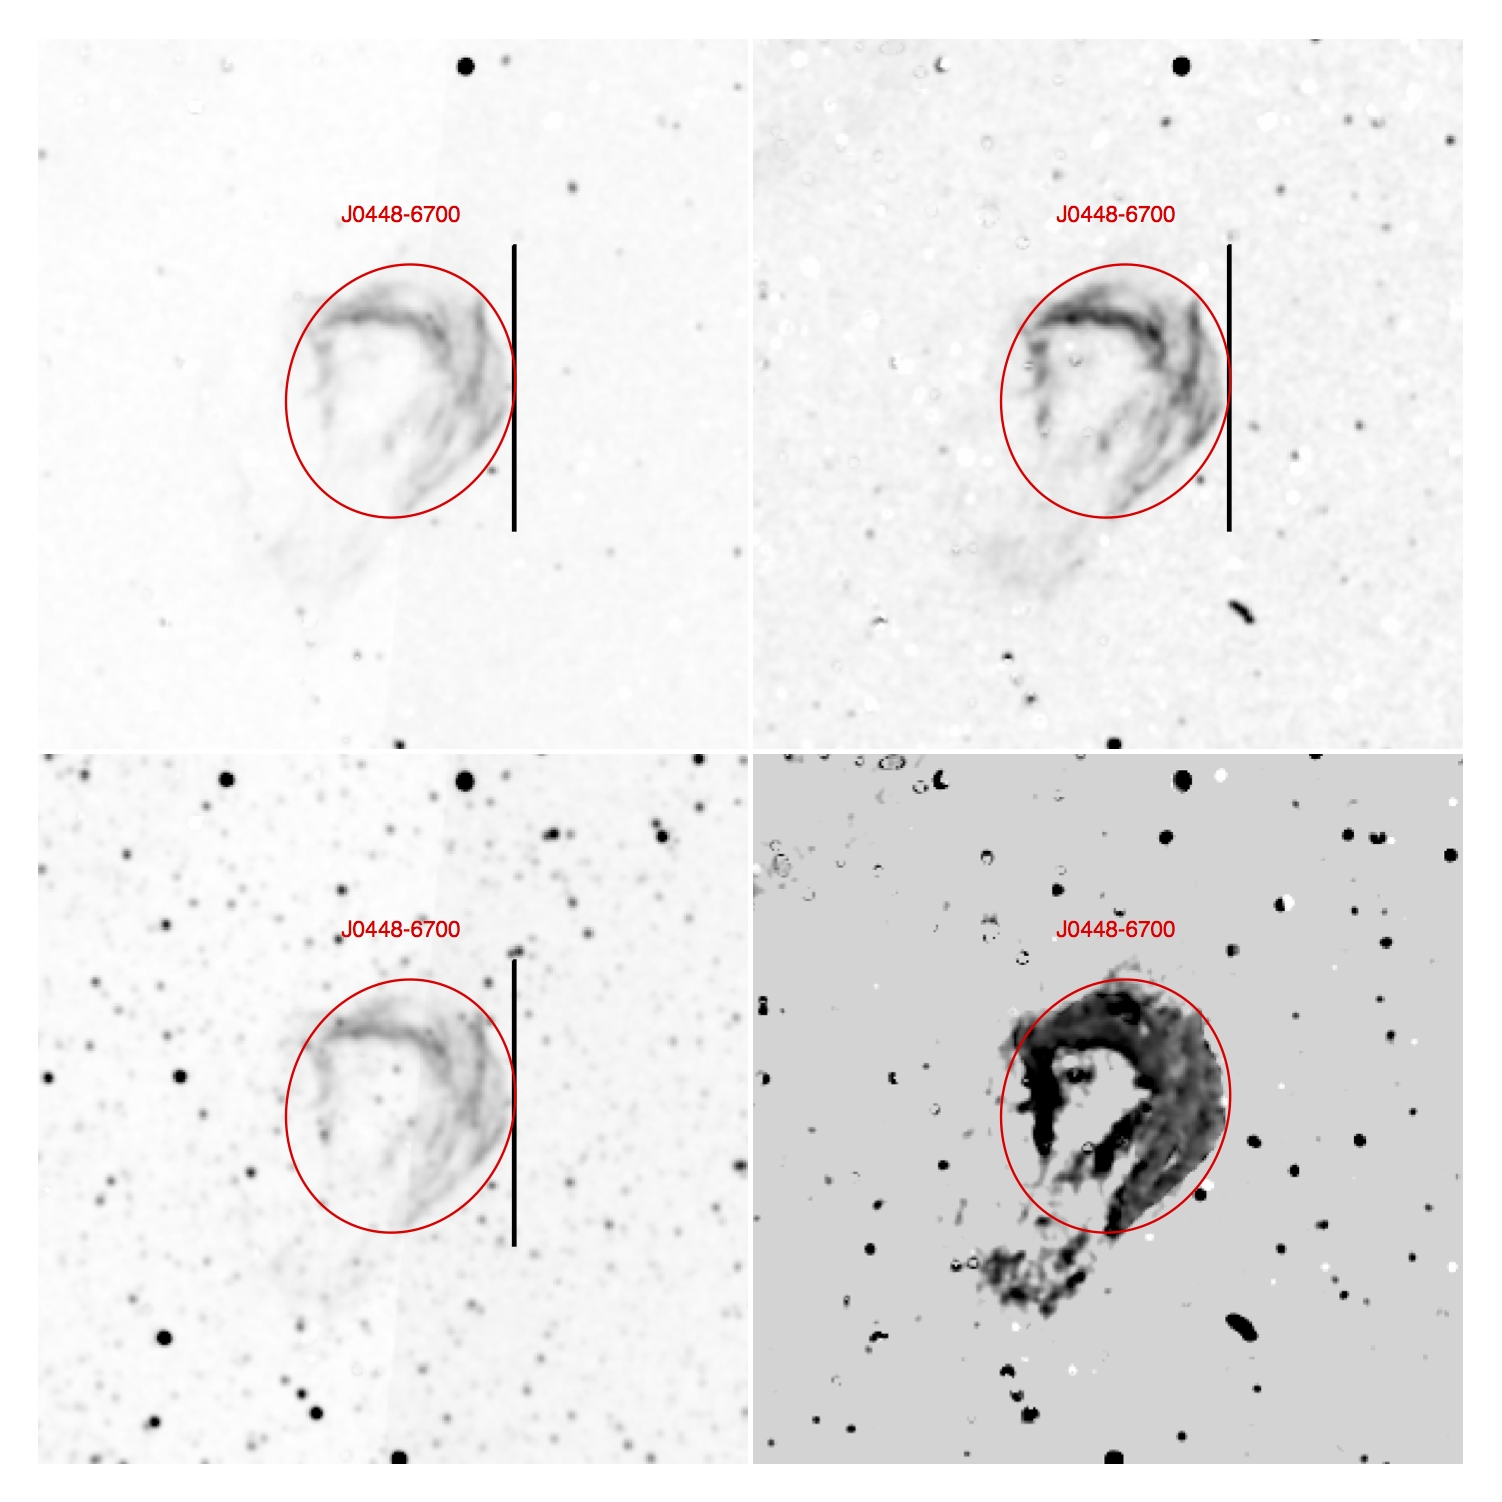
\includegraphics[width=10.05cm]{snapshots/J0448-6700.png}
\end{figure}

\newpage
{\bf J0449-6920}

Slit Center:   4:49:12.574     -69:20:18.499     N-S

Scan:  East

Scan rate:  

Date/Frames:

Exposure Times:  

\begin{figure}
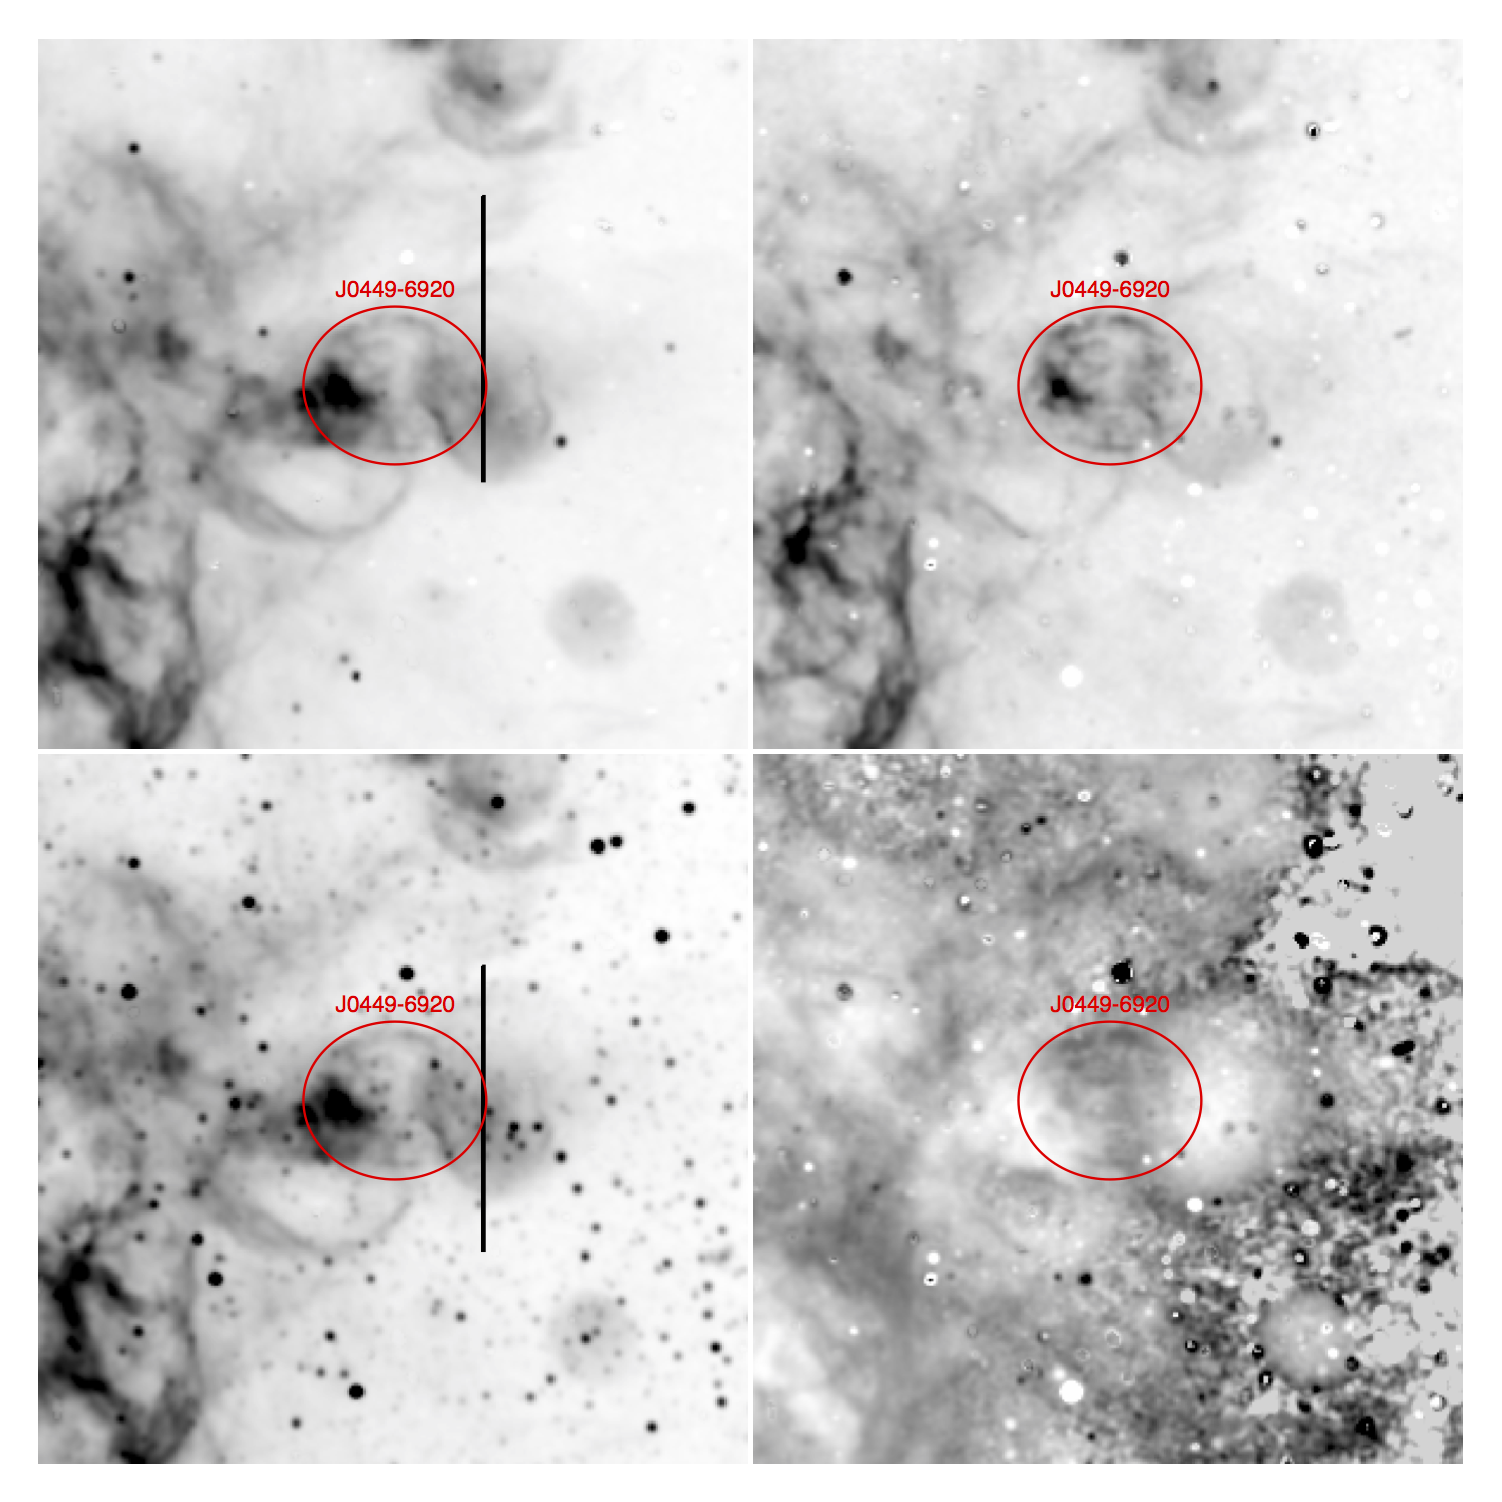
\includegraphics[width=10.05cm]{snapshots/J0449-6920.png}
\end{figure}

\newpage
{\bf J0453-6655}

Slit Center:   4:52:54.512    -66:54:46.762     N-S

Scan:  East

Scan rate:  

Date/Frames:

Exposure Times:  

\begin{figure}
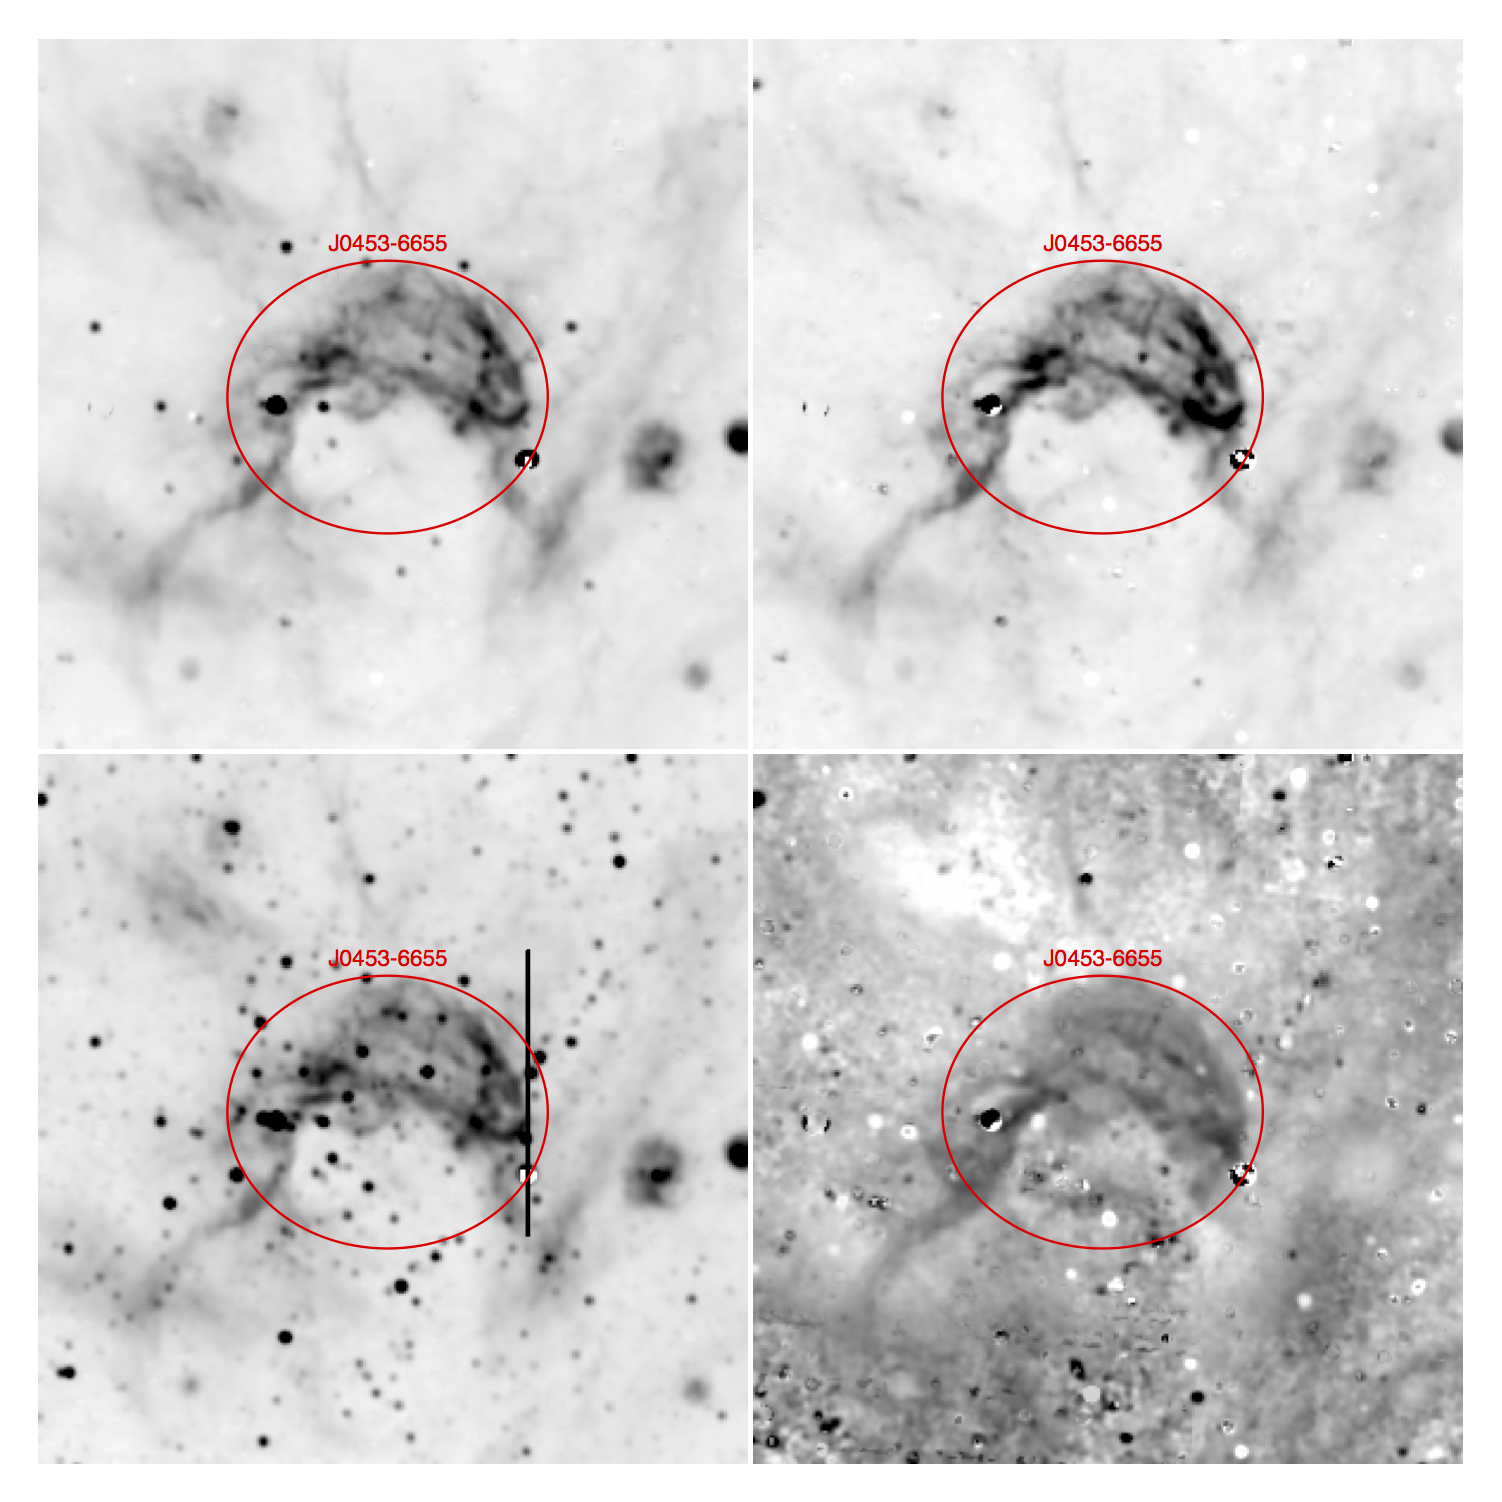
\includegraphics[width=10.05cm]{snapshots/J0453-6655.png}
\end{figure}

\newpage
{\bf J0453-6829 = B0453-685}

Slit Center:   4:53:14.089    -68:29:43.361     N-S

Scan:  East

Scan rate:  

Date/Frames:

Exposure Times:  

\begin{figure}
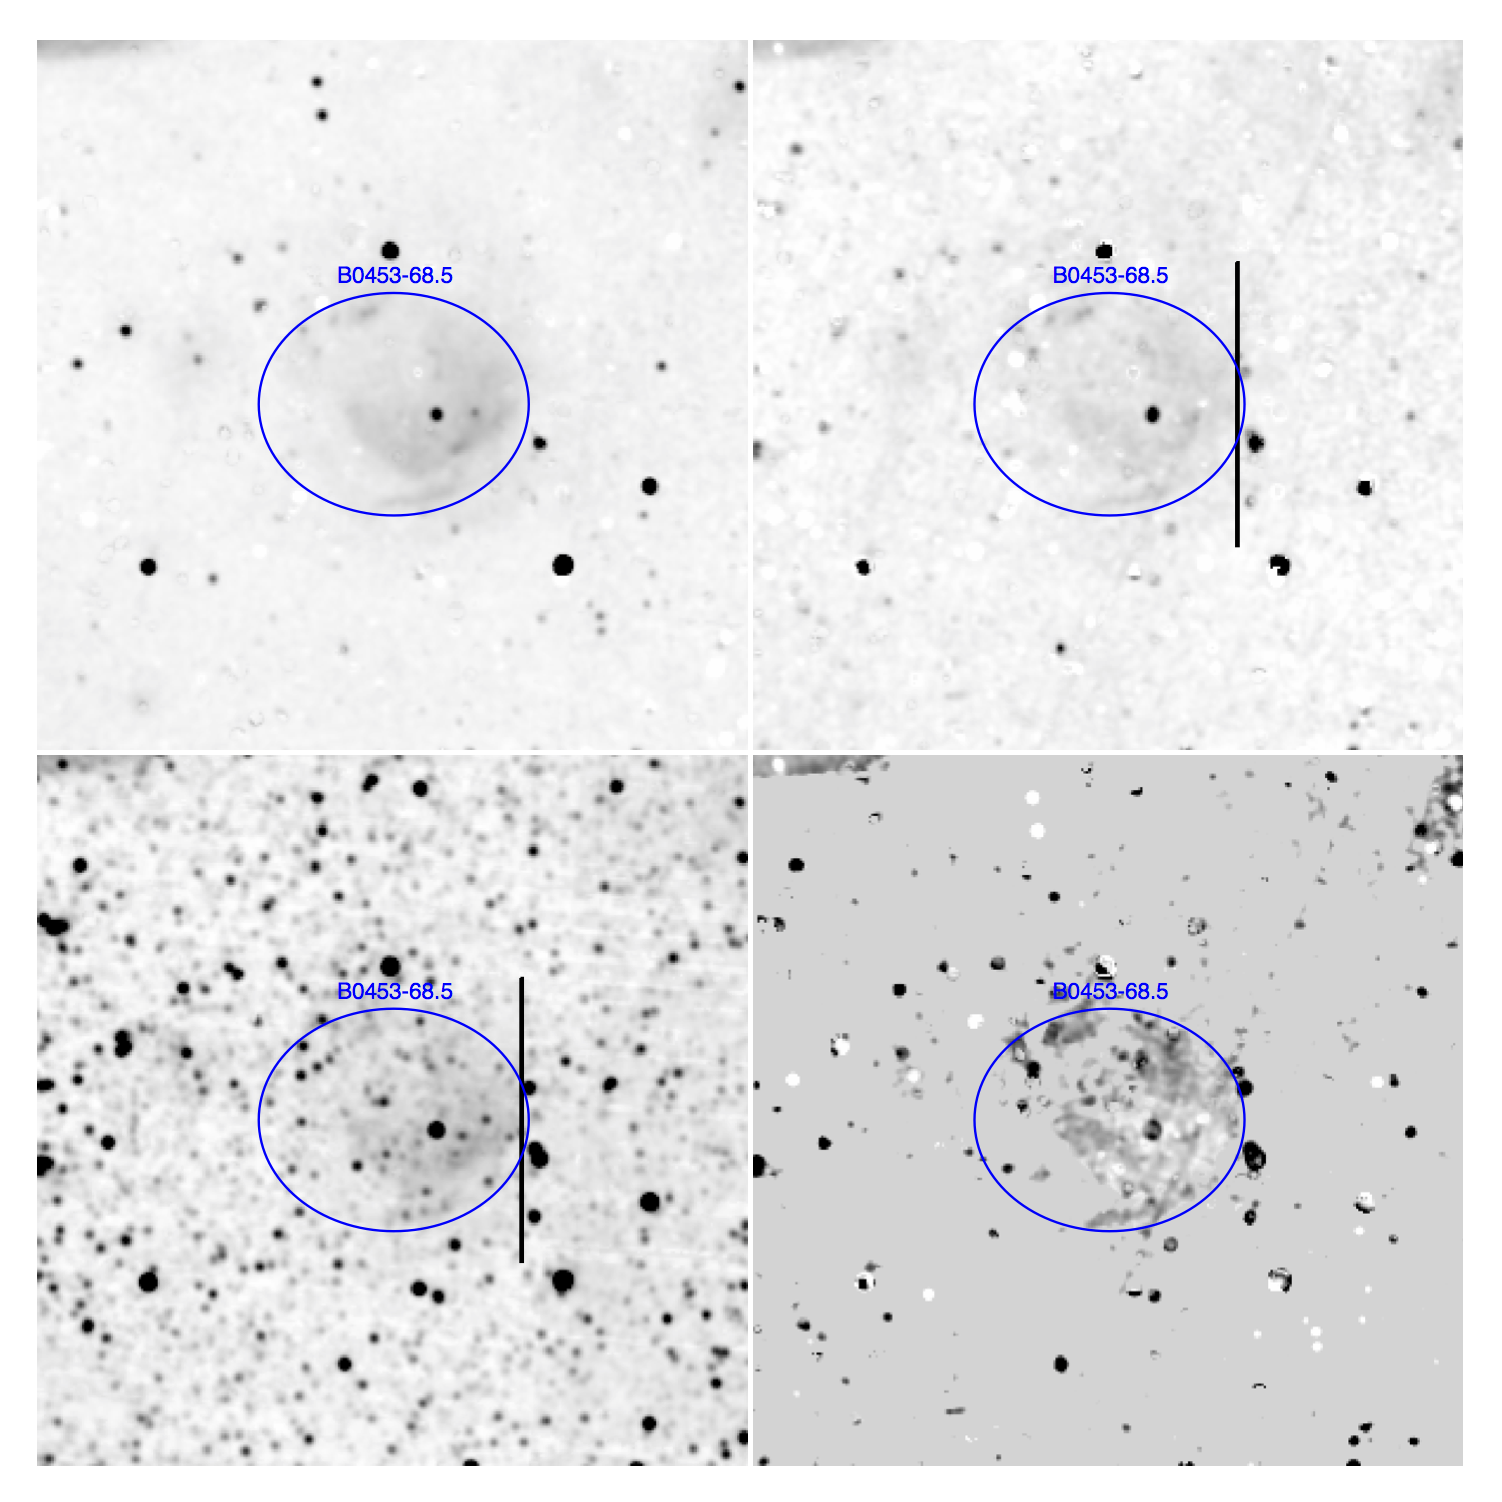
\includegraphics[width=10.05cm]{snapshots/B0453-685.png}
\end{figure}

\newpage
{\bf JJ0454-7003 (new)}

Slit Center:   4:54:07.473      -70:04:07.707     N-S

Scan:  East

Scan rate:  

Date/Frames:

Exposure Times:  

\begin{figure}
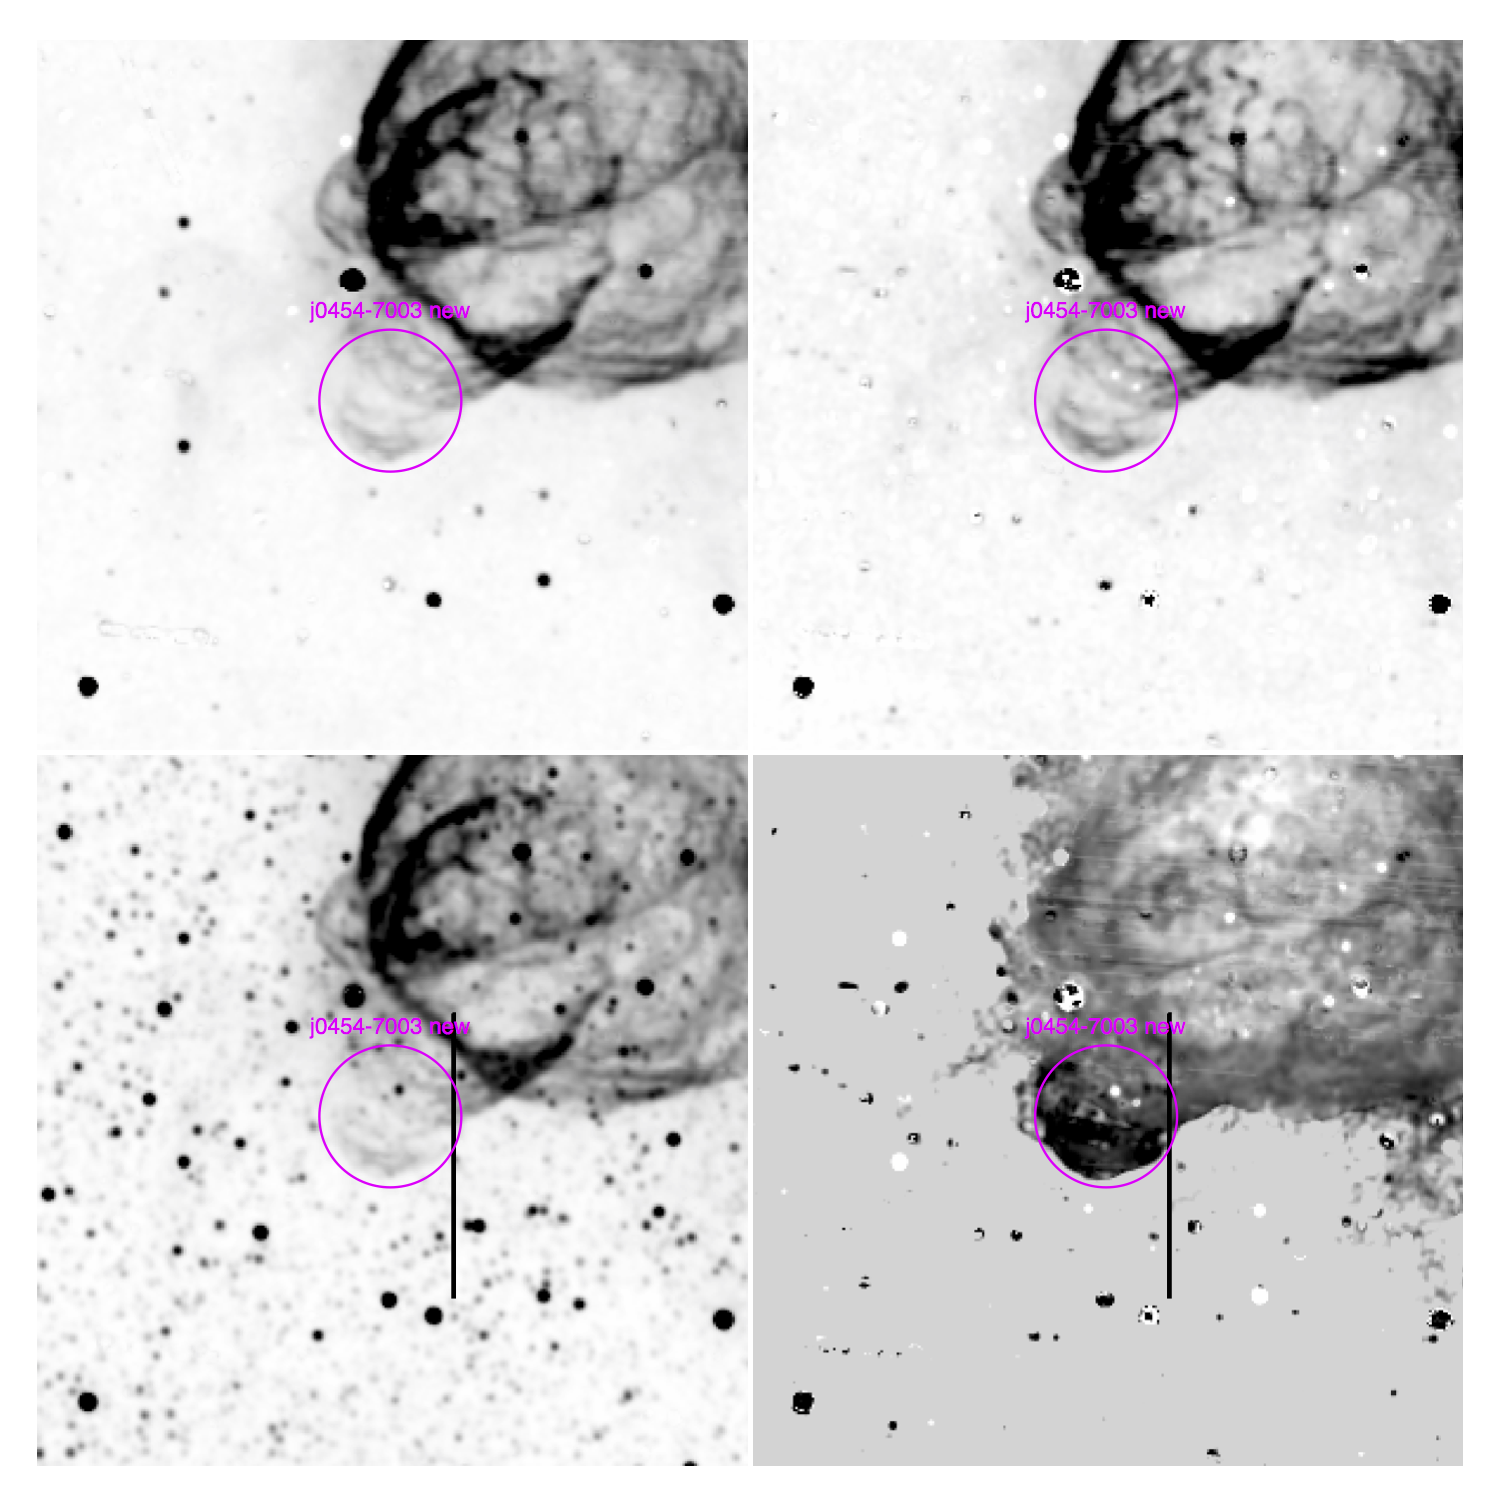
\includegraphics[width=10.05cm]{snapshots/J0454-7003.png}
\end{figure}

\newpage
{\bf J0454-6712 = N9}

Slit Center:   4:54:17.308    -67:12:55.968     N-S

Scan:  East

Scan rate:  

Date/Frames:

Exposure Times:  

\begin{figure}
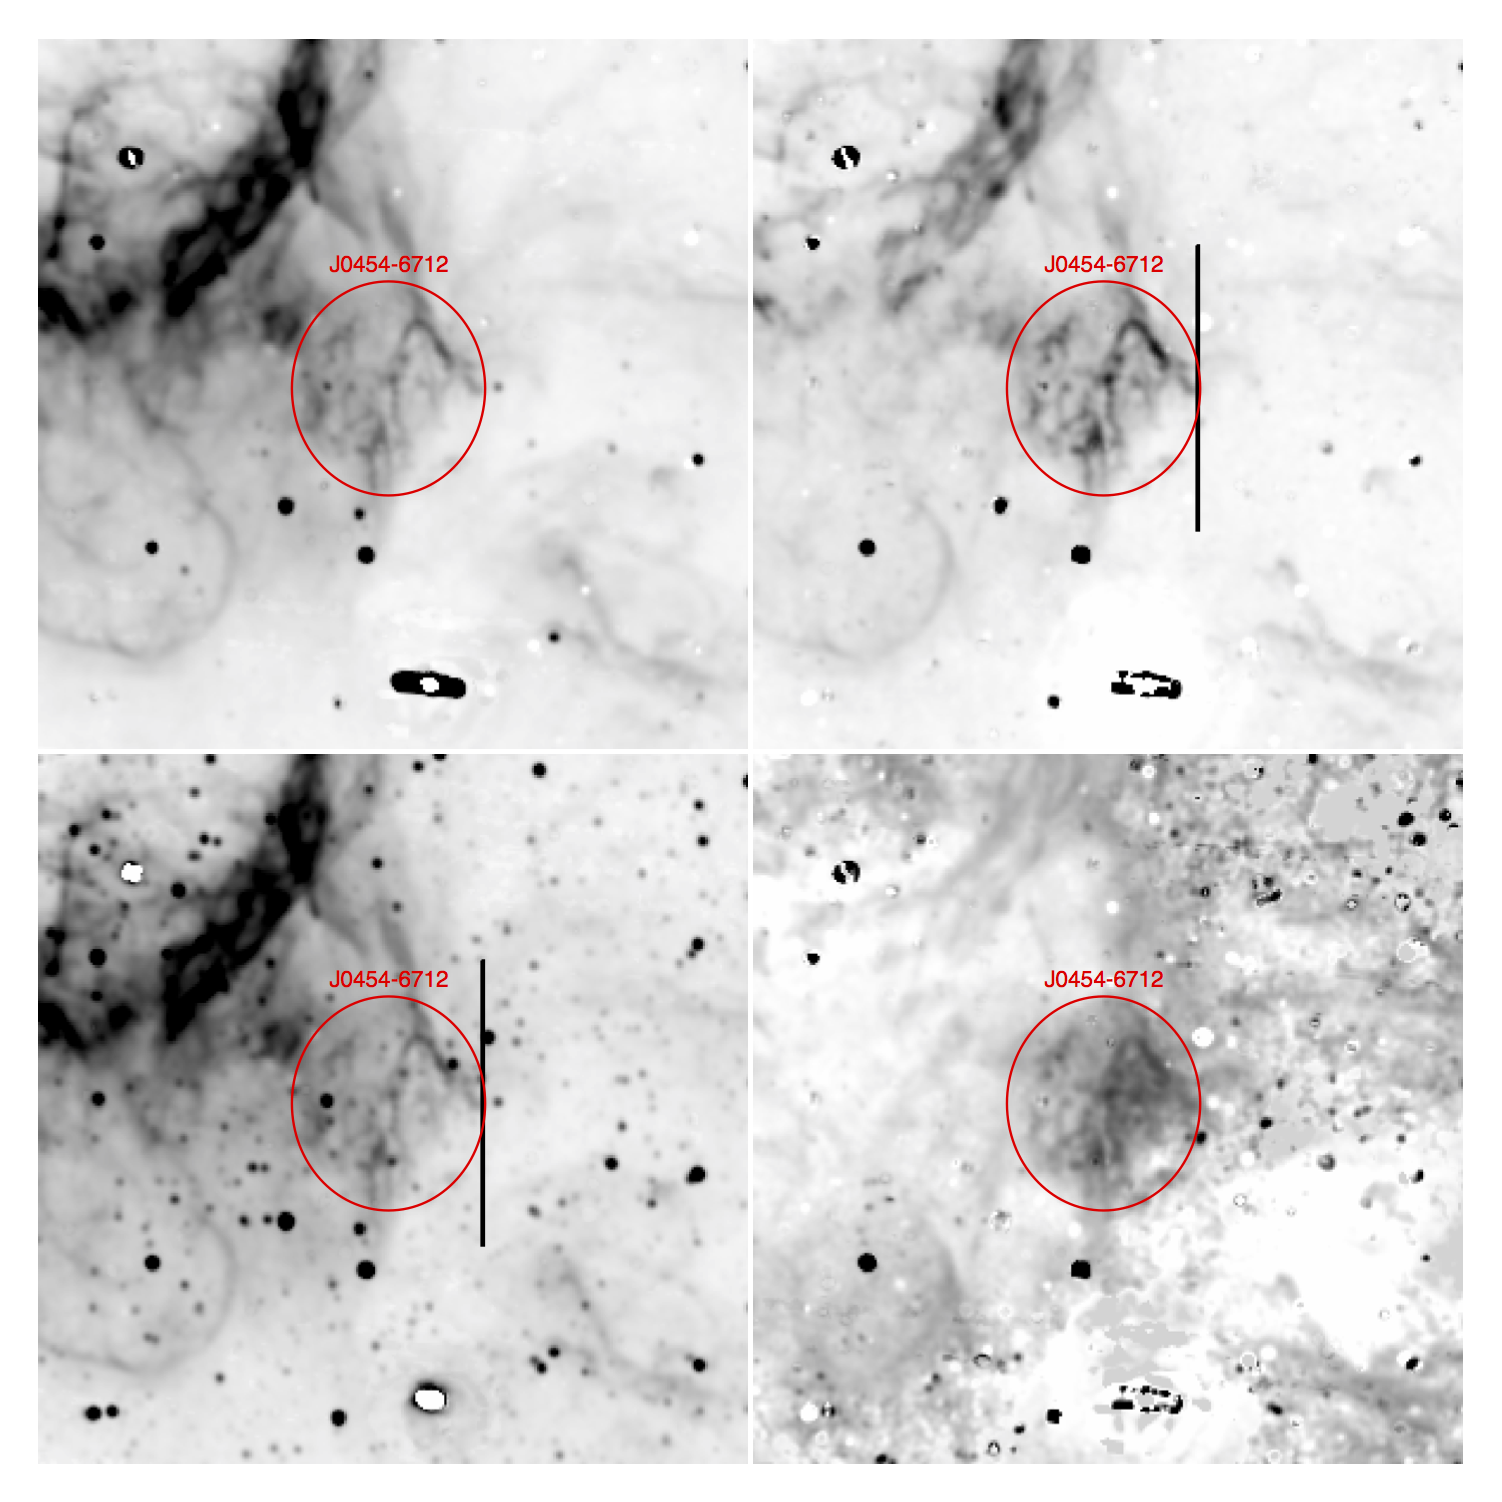
\includegraphics[width=10.05cm]{snapshots/J0454-6712.png}
\end{figure}

\newpage
{\bf J0454-6625 = B0454-665 = N11L}

Slit Center:   4:54:43.033    -66:25:31.629     N-S

Scan:  East

Scan rate:  

Date/Frames:

Exposure Times:  

\begin{figure}
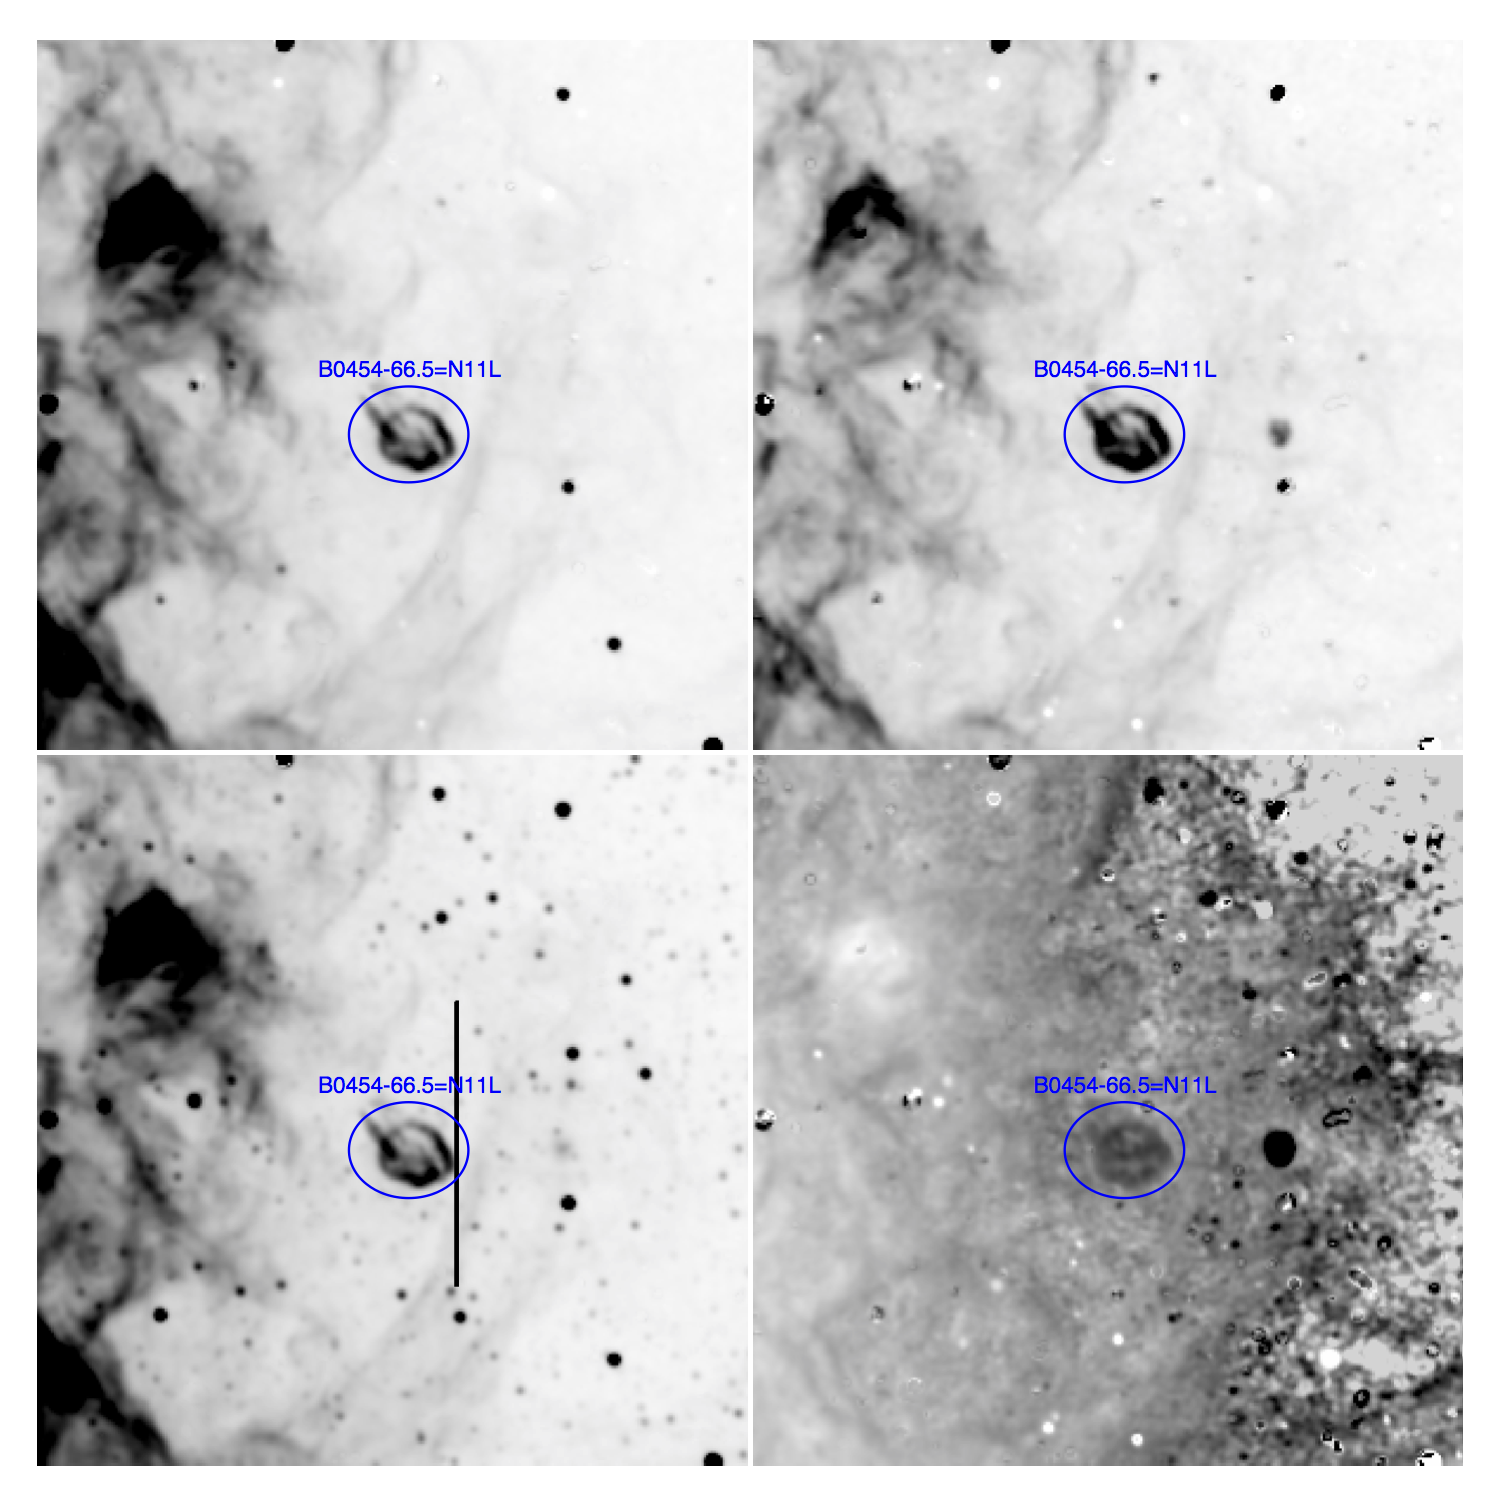
\includegraphics[width=10.05cm]{snapshots/B0454-665.png}
\end{figure}

\newpage
{\bf J0455-6839 = B0455-687 = N86}

Slit Center:   4:55:46.302    -68:37:41.817     E-W

Scan:  South

Scan rate:  

Date/Frames:

Exposure Times:  

\begin{figure}
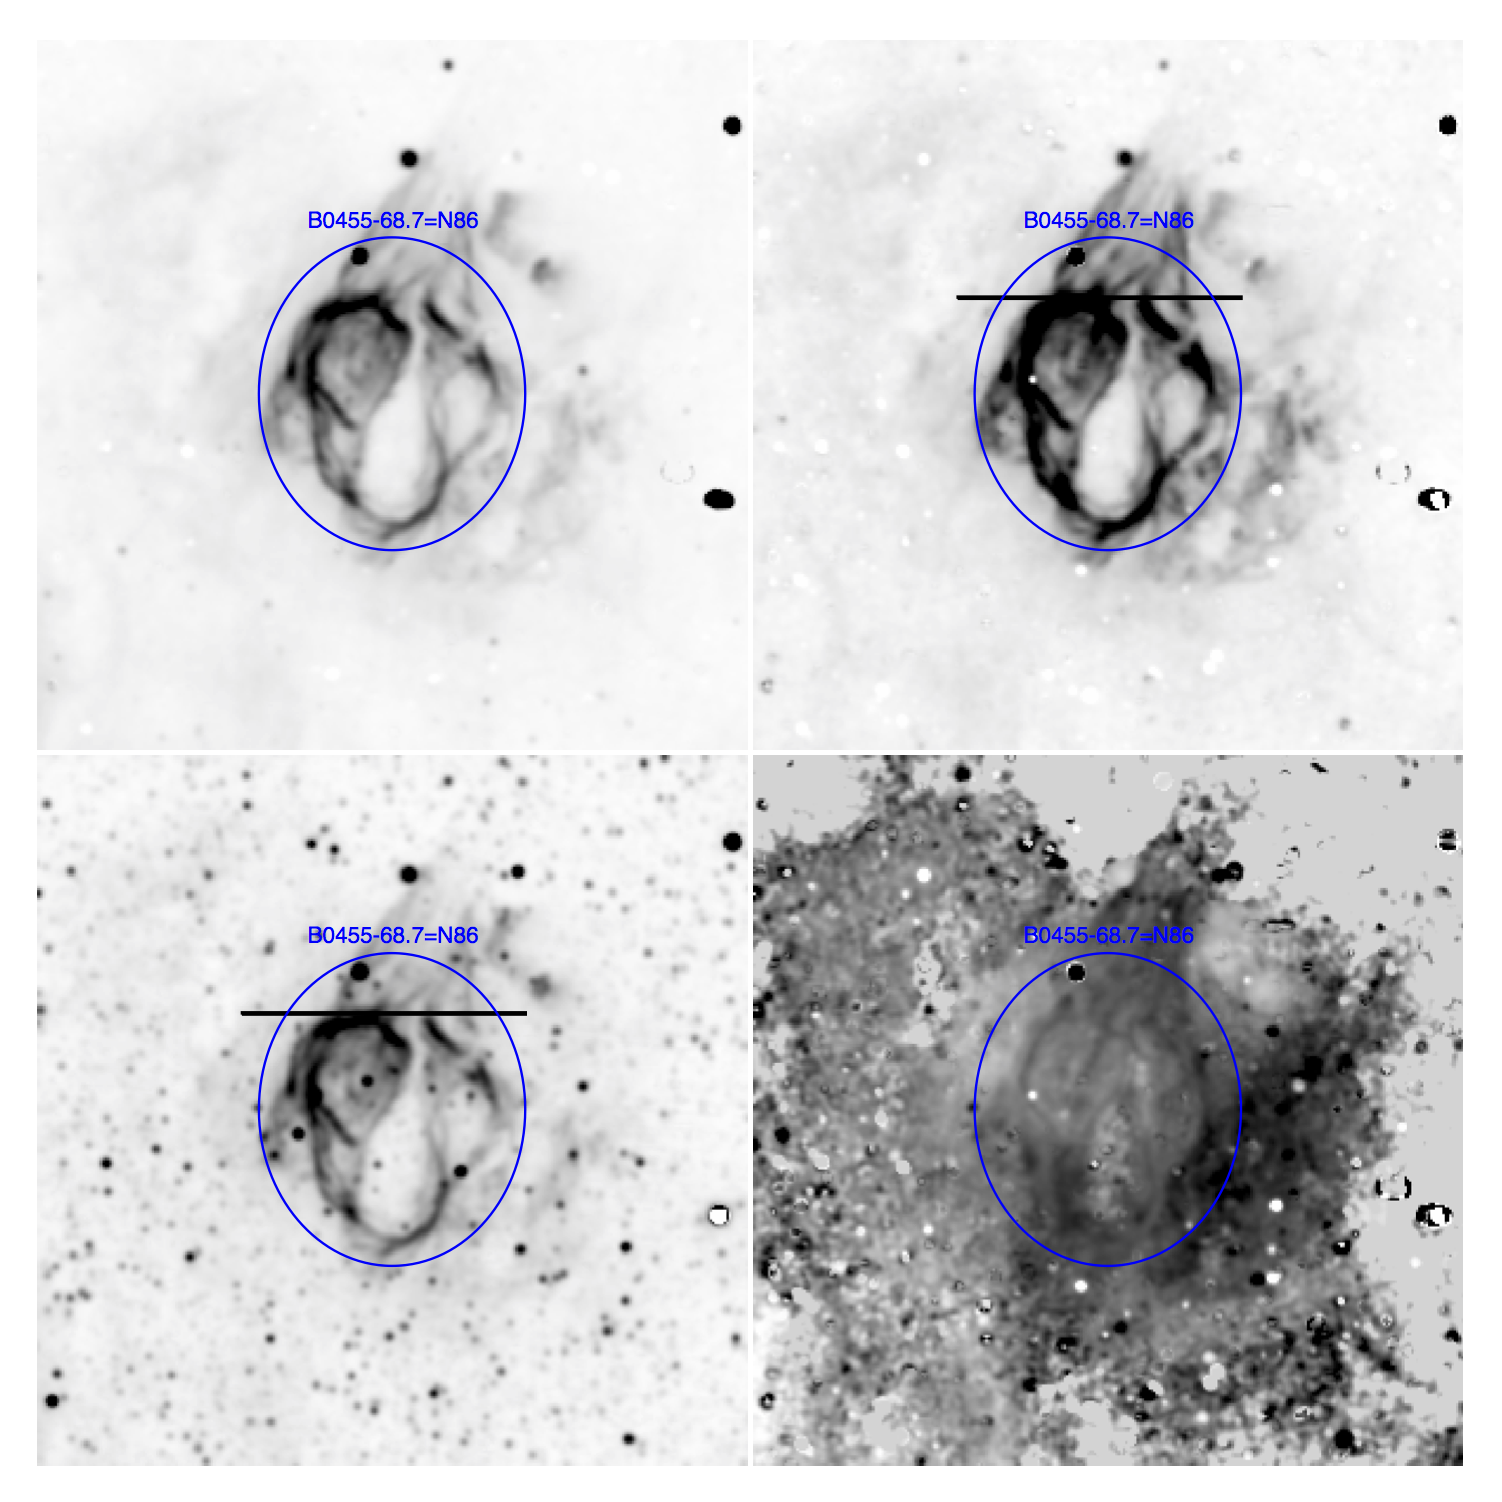
\includegraphics[width=10.05cm]{snapshots/B0455-687.png}
\end{figure}


\newpage
{\bf J0459-7008 = B0500-702 = N186D}

Slit Center:   4:59:43.935    -70:07:36.307     N-S

Scan:  East

Scan rate:  

Date/Frames:

Exposure Times:  

\begin{figure}
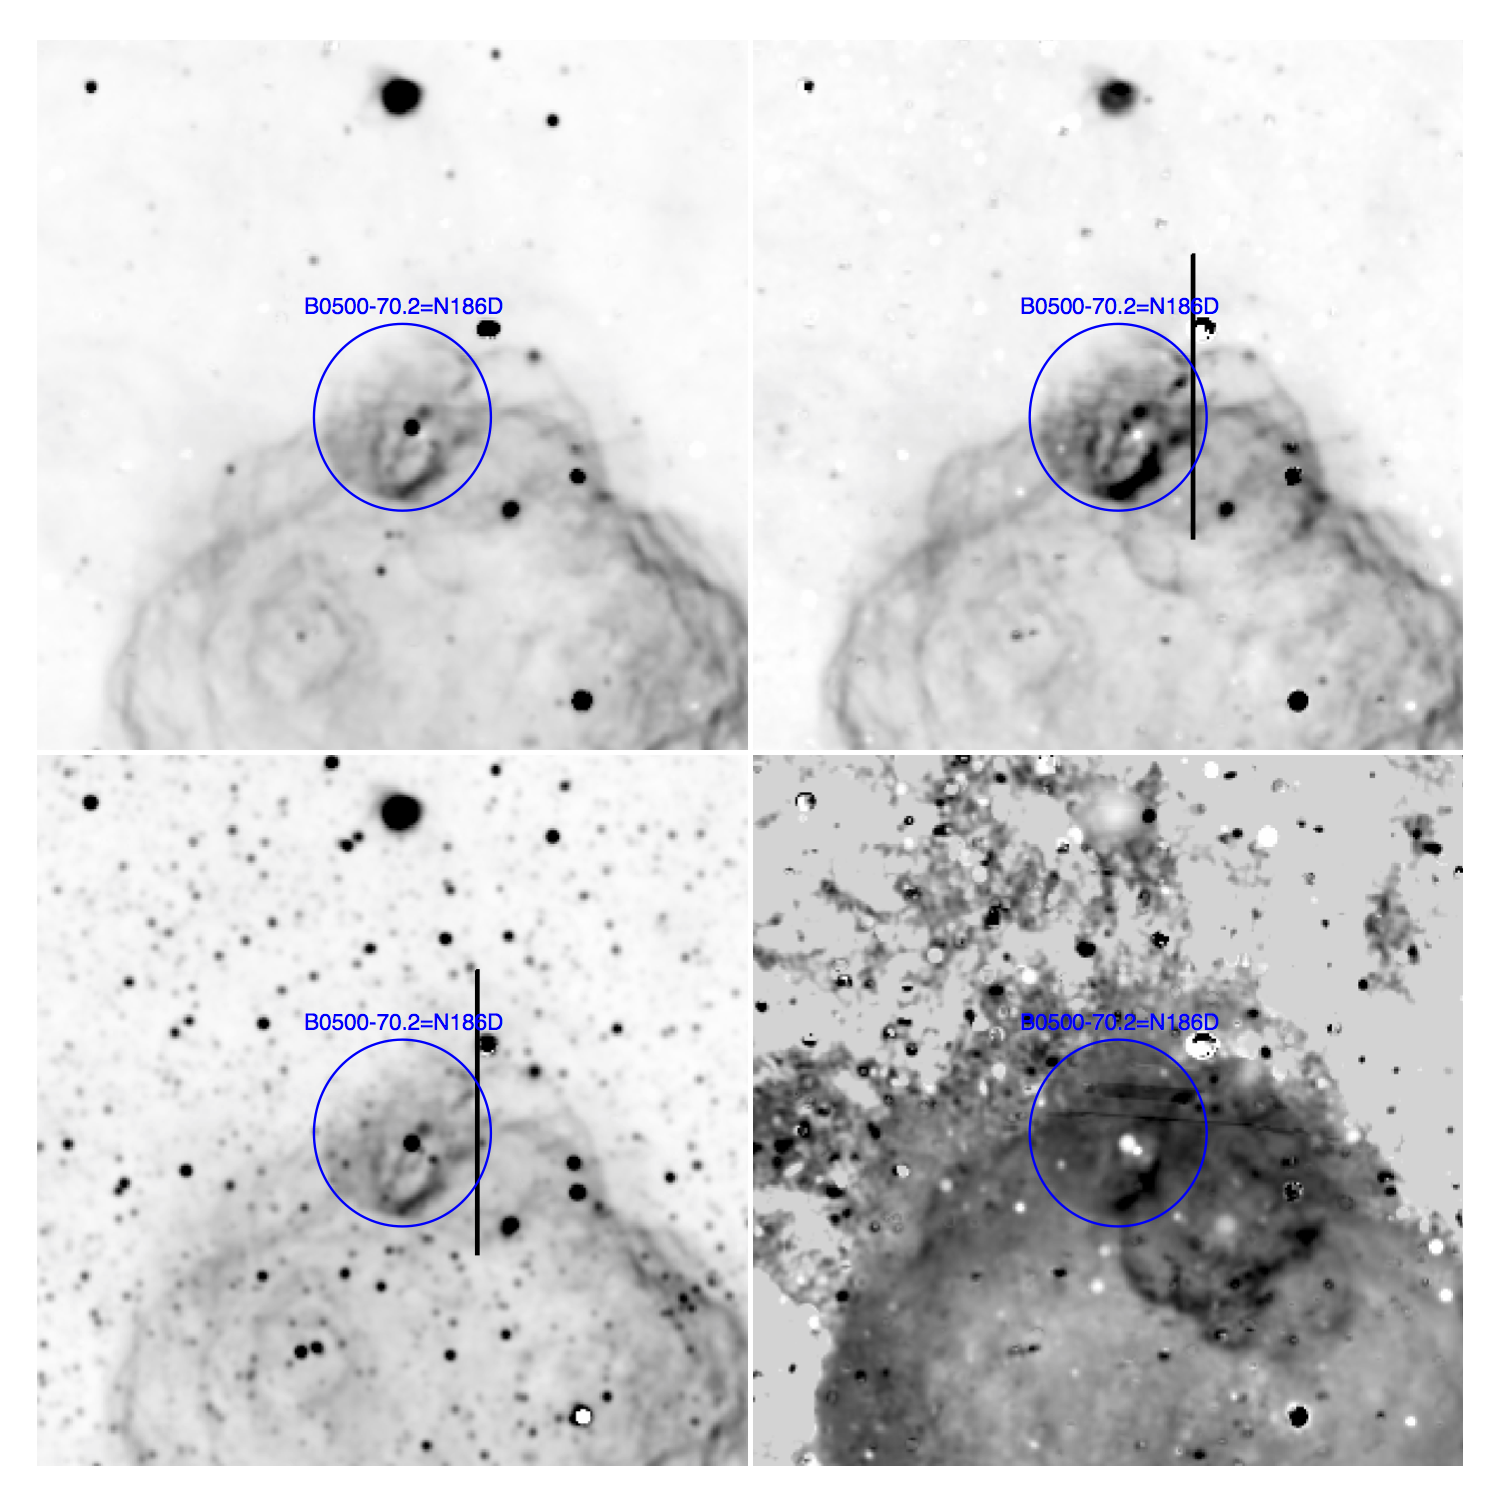
\includegraphics[width=10.05cm]{snapshots/B0500-702.png}
\end{figure}

\newpage
{\bf J0505-6752 = B0505-679 = DEML71}  (Balmer-dominated)

Slit Center:   5:05:35.913    -67:52:34.226     N-S

Scan:  East

Scan rate:  

Date/Frames:

Exposure Times:  

\begin{figure}
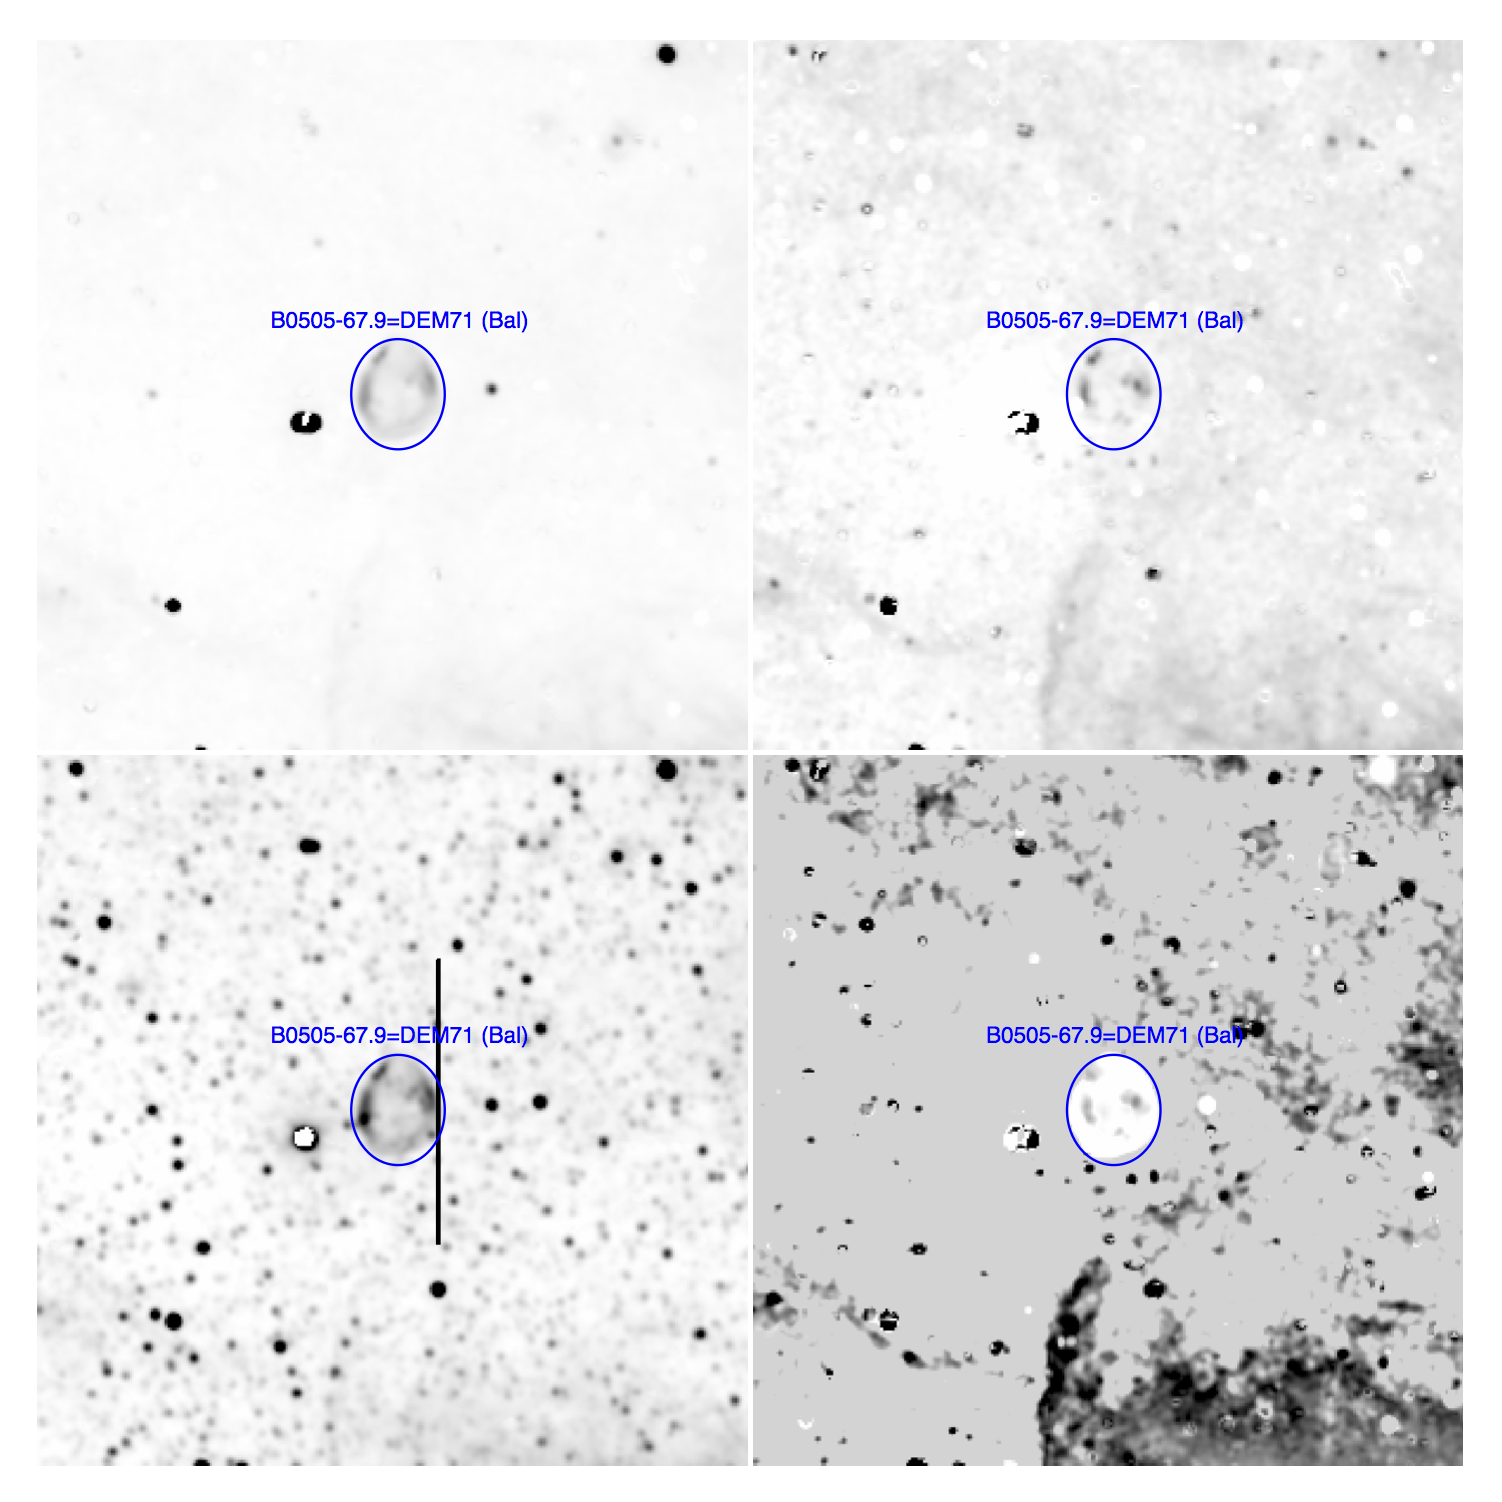
\includegraphics[width=10.05cm]{snapshots/B0505-679.png}
\end{figure}

\newpage
{\bf J0505-6801 = B0506-68.0 = N23}  
 
Slit Center:   5:05:46.637    -68:01:47.761     N-S

Scan:  East

Scan rate:  

Date/Frames:

Exposure Times:  

\begin{figure}
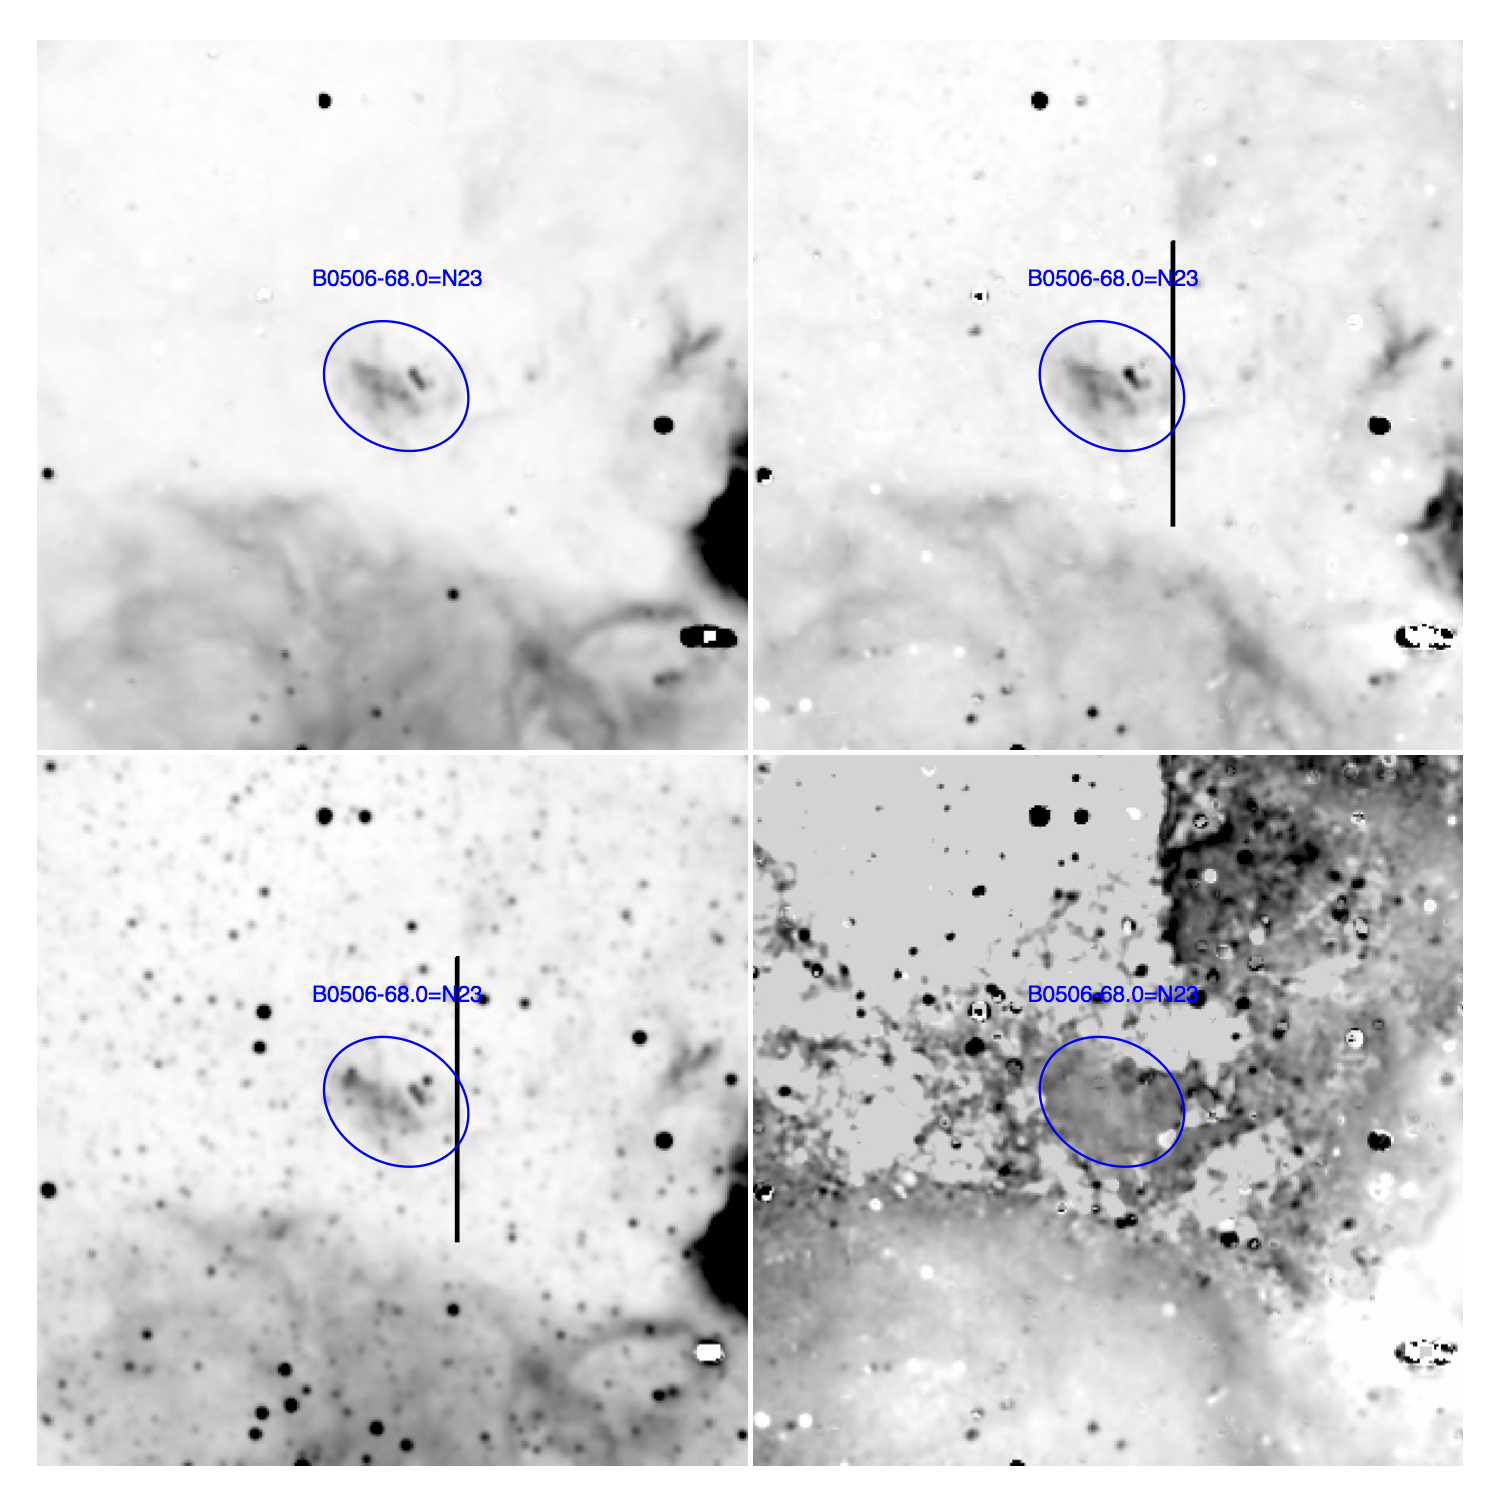
\includegraphics[width=10.05cm]{snapshots/B0506-680.png}
\end{figure}

\newpage
{\bf J0506-7025 = DEML80}  
 
Slit Center:   5:06:30.133    -70:25:09.366     N-S

Scan:  East

Scan rate:  

Date/Frames:

Exposure Times:  

\begin{figure}
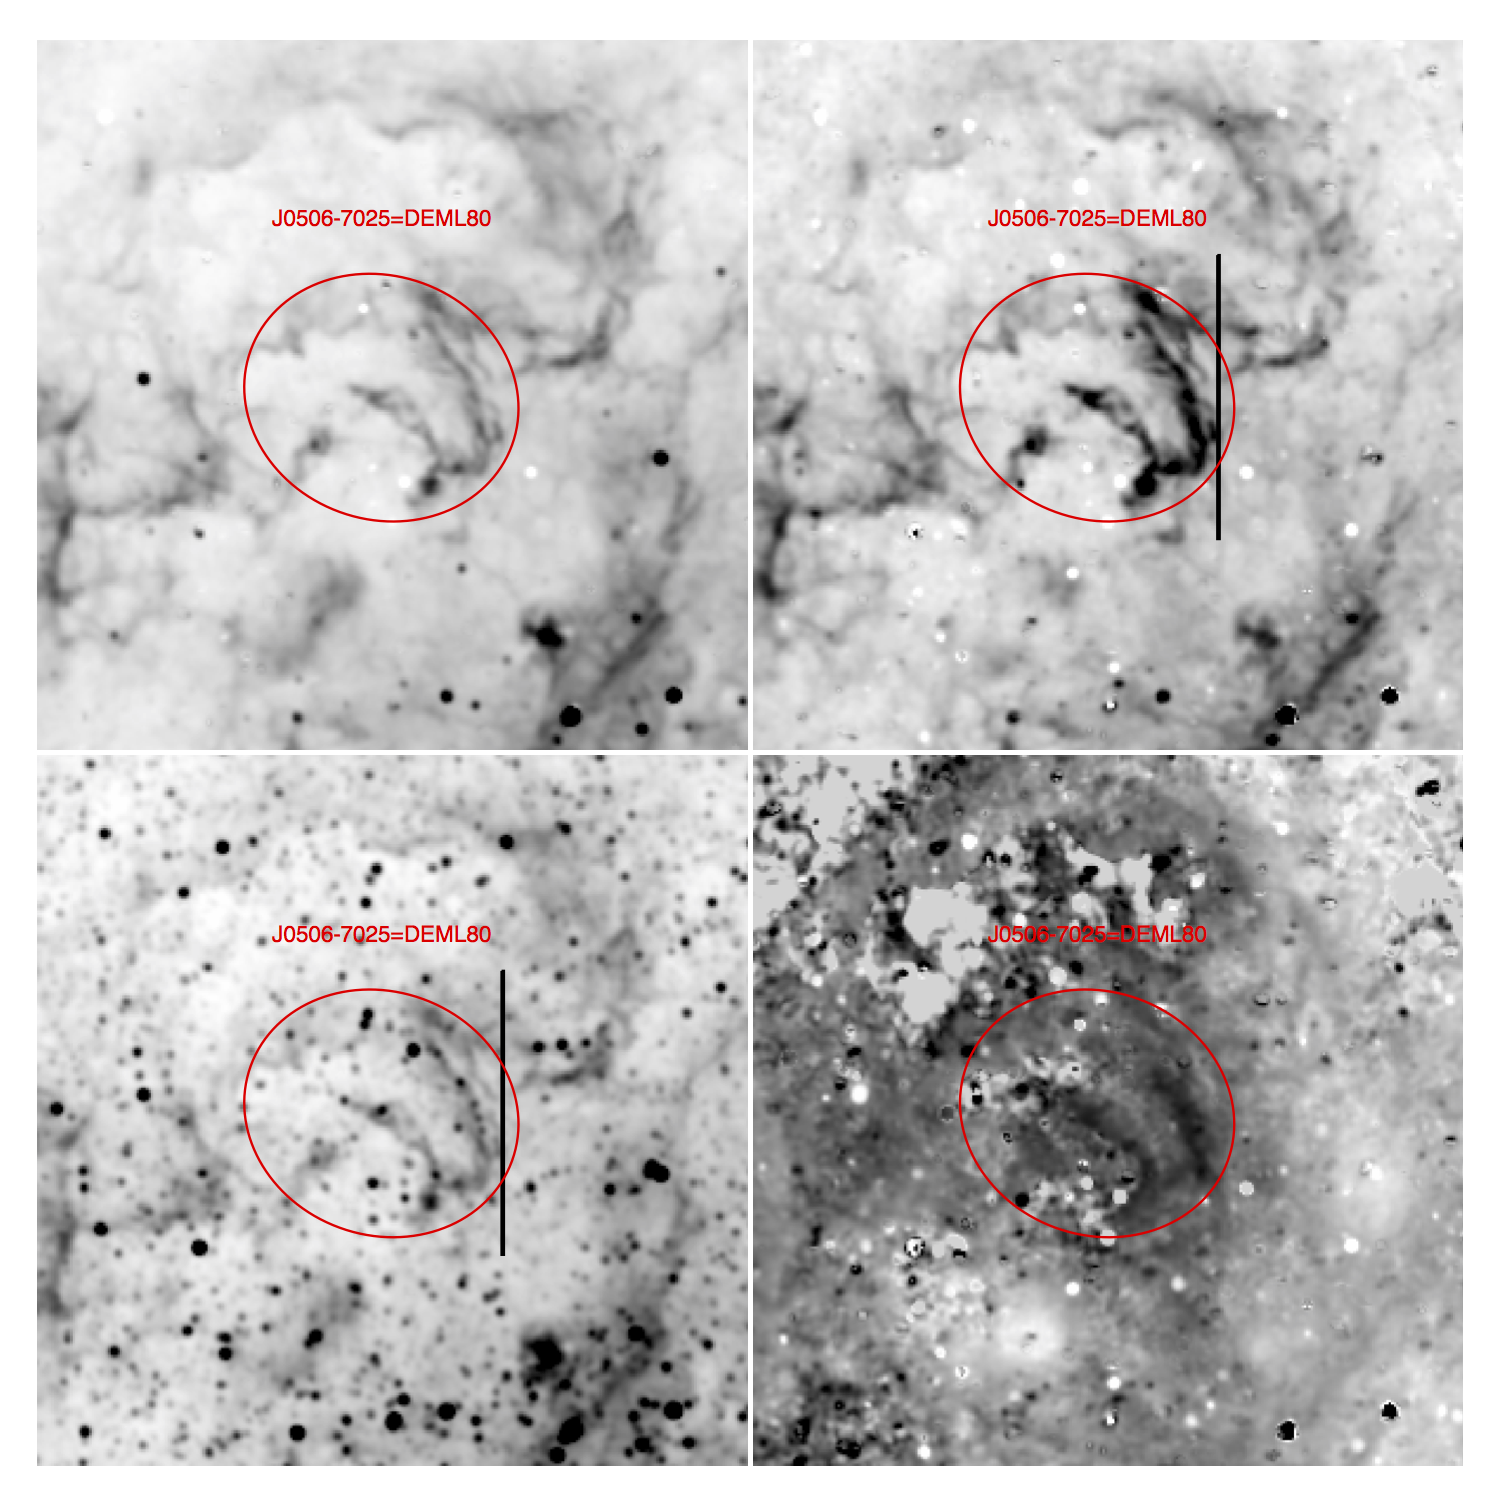
\includegraphics[width=10.05cm]{snapshots/J0506-7025.png}
\end{figure}

\newpage
{\bf J0507-7110 new}  
 
Slit Center:   5:07:09.621   -71:10:32.881     N-S

Scan:  East

Scan rate:  

Date/Frames:

Exposure Times:  

\begin{figure}
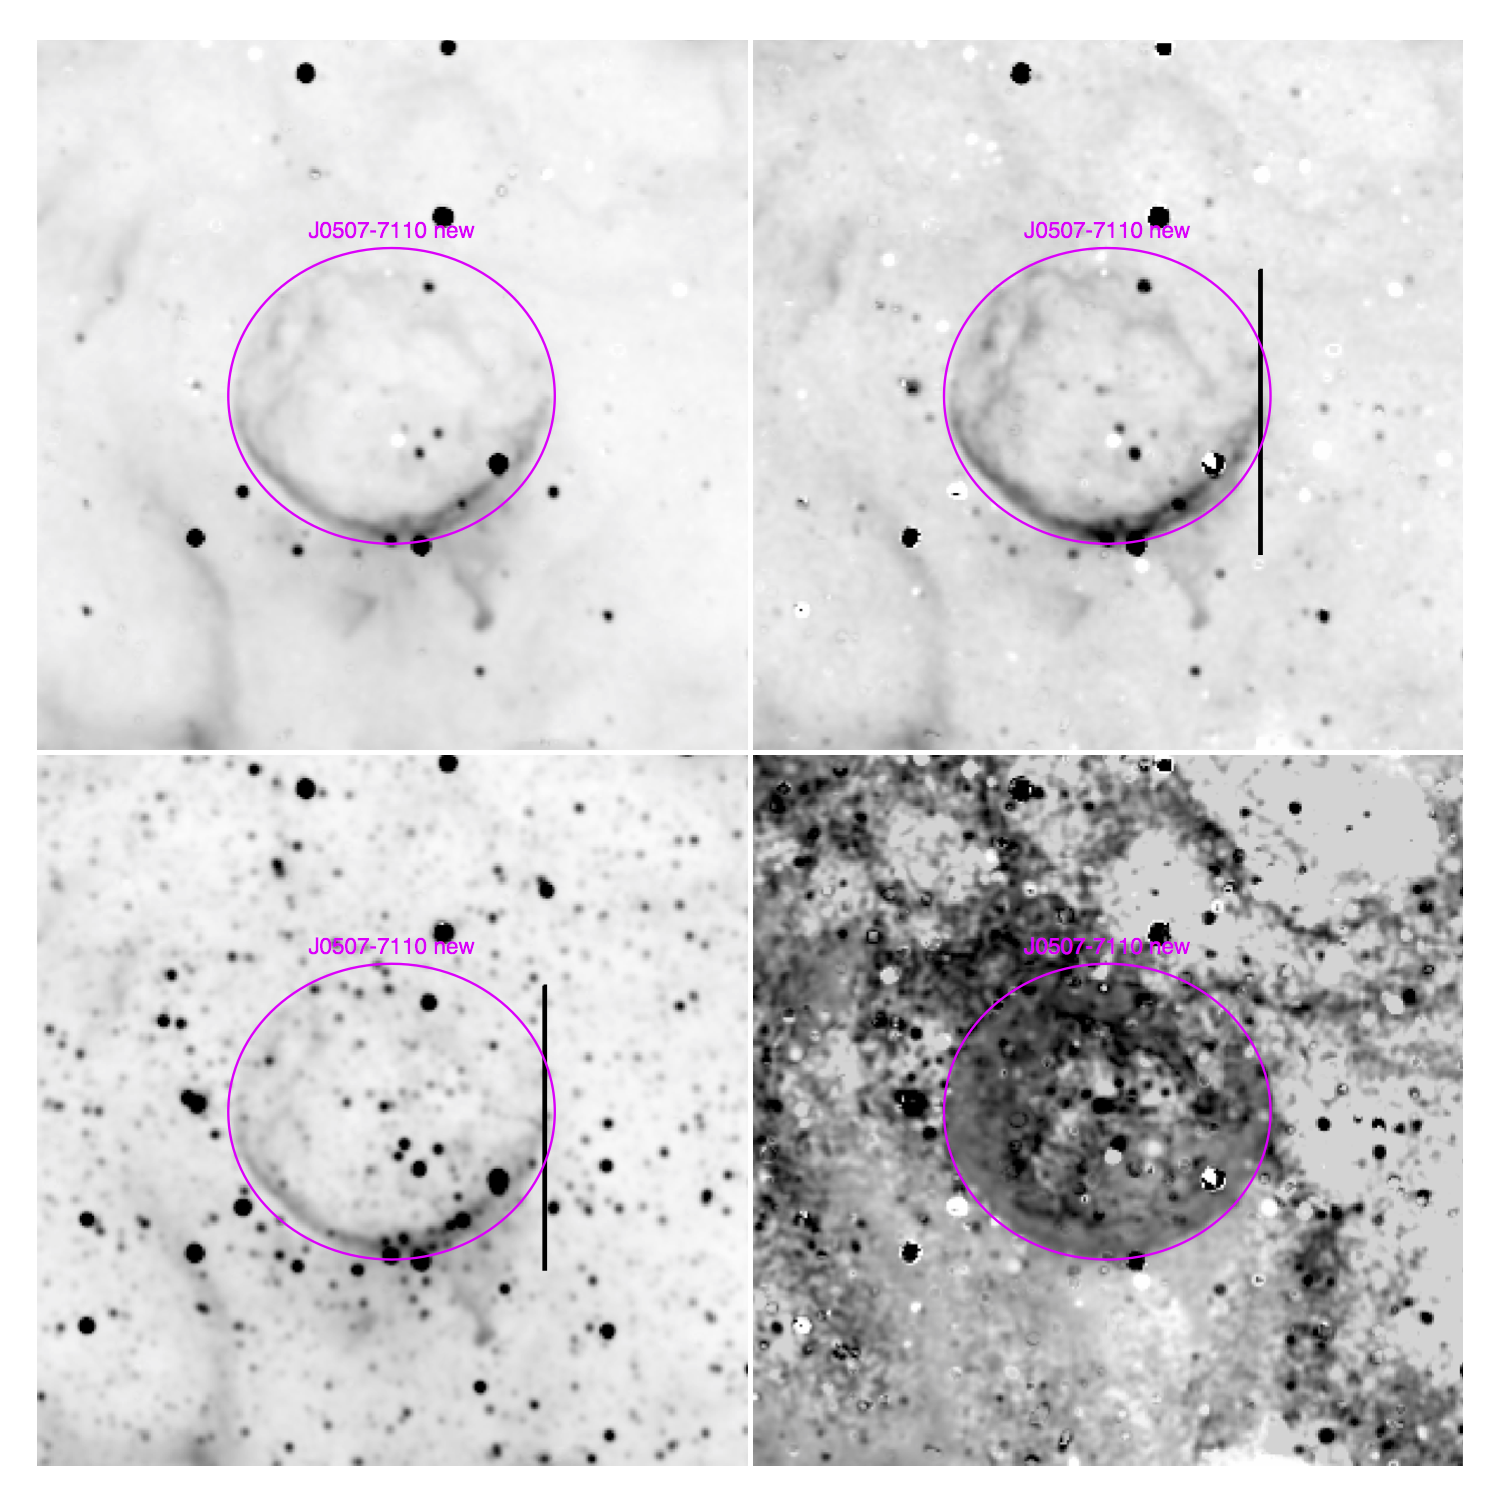
\includegraphics[width=10.05cm]{snapshots/J0507-7110.png}
\end{figure}

\newpage
{\bf J0508-6902}  
 
Slit Center:   5:08:26.193   -69:04:07.007     E-W

Scan:  North

Scan rate:  

Date/Frames:

Exposure Times:  

\begin{figure}
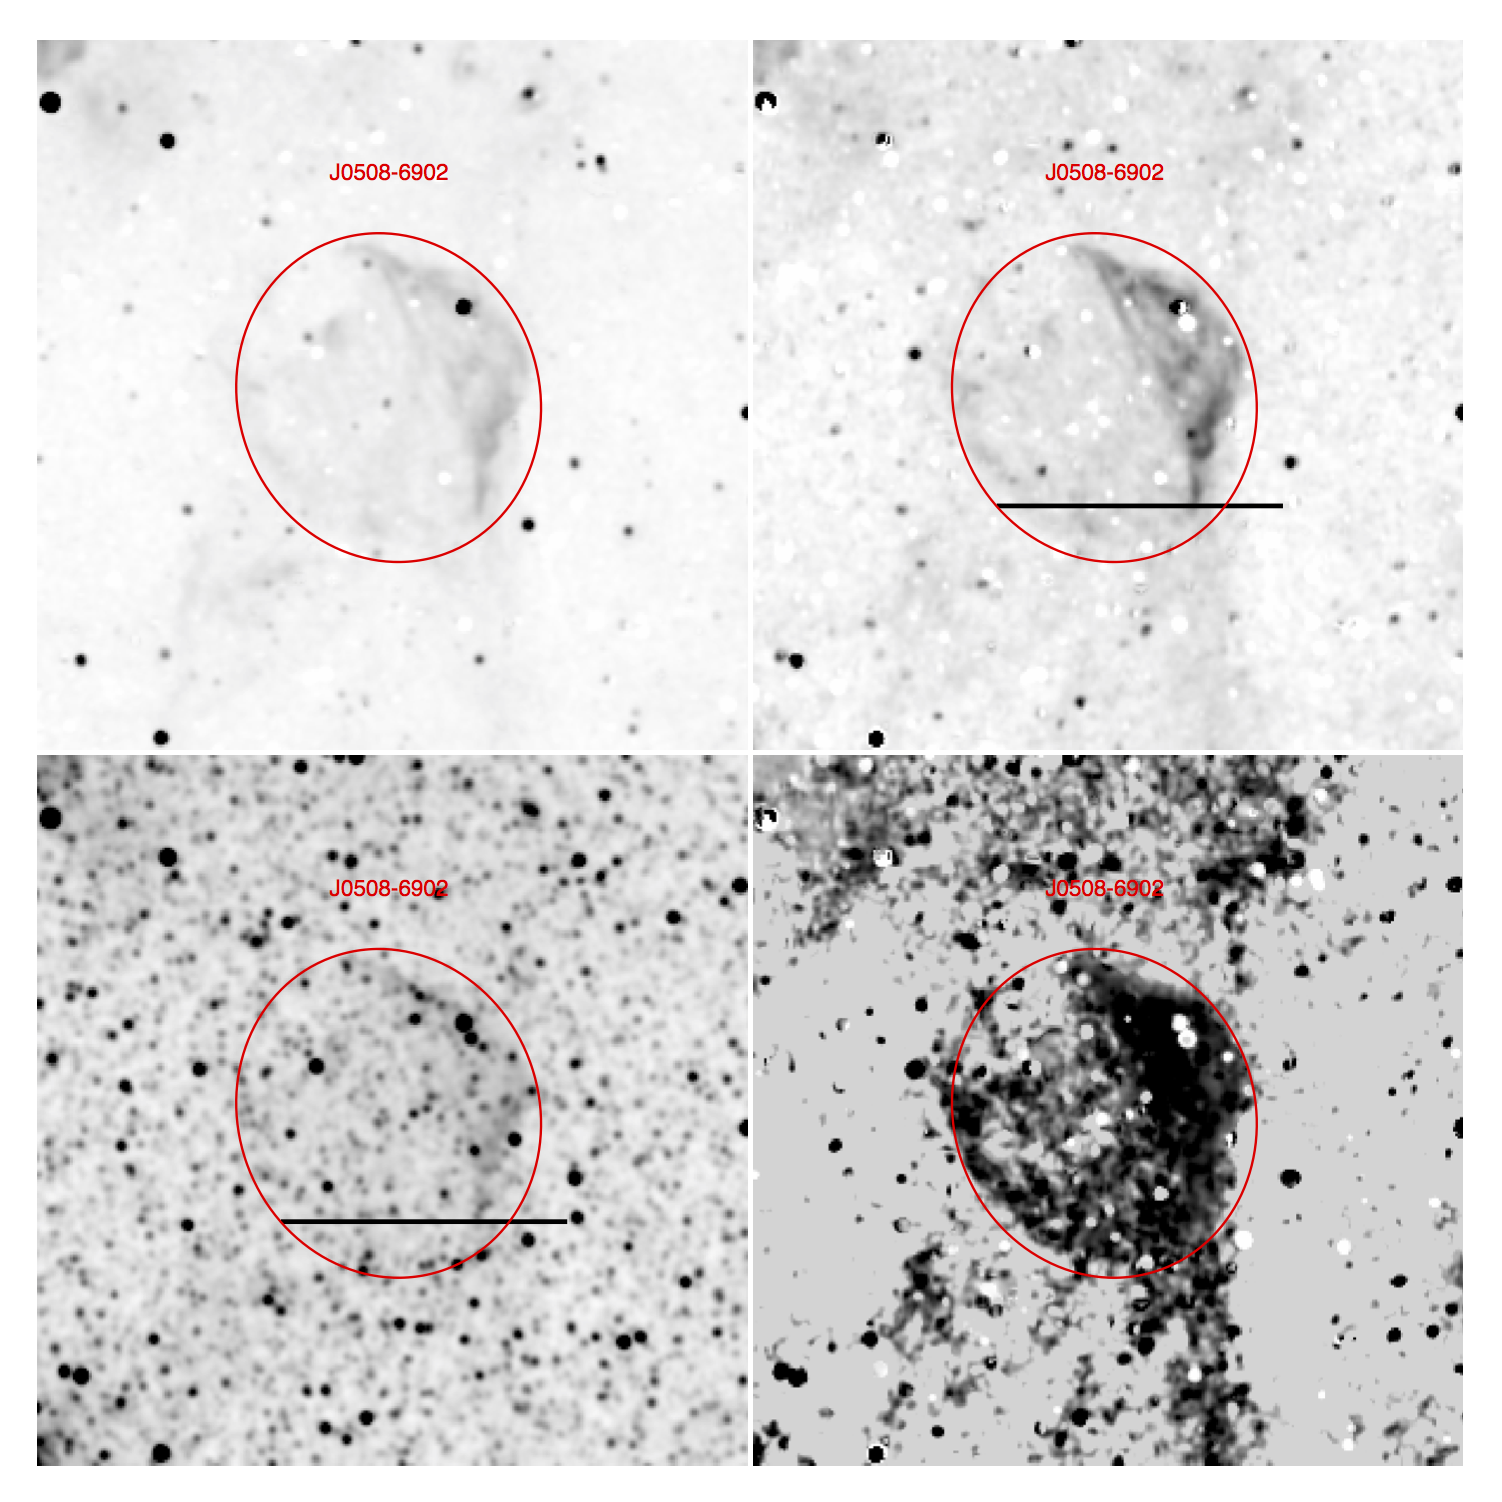
\includegraphics[width=10.05cm]{snapshots/J0508-6902.png}
\end{figure}

\newpage
{\bf J508-6843 = B0509-68.7 = N103B}  (Panels $5^\prime$ square)
 
Slit Center:   5:08:57.318   -68:43:28.685     N-S 

Scan:  East

Scan rate:  

Date/Frames:

Exposure Times:  

\begin{figure}
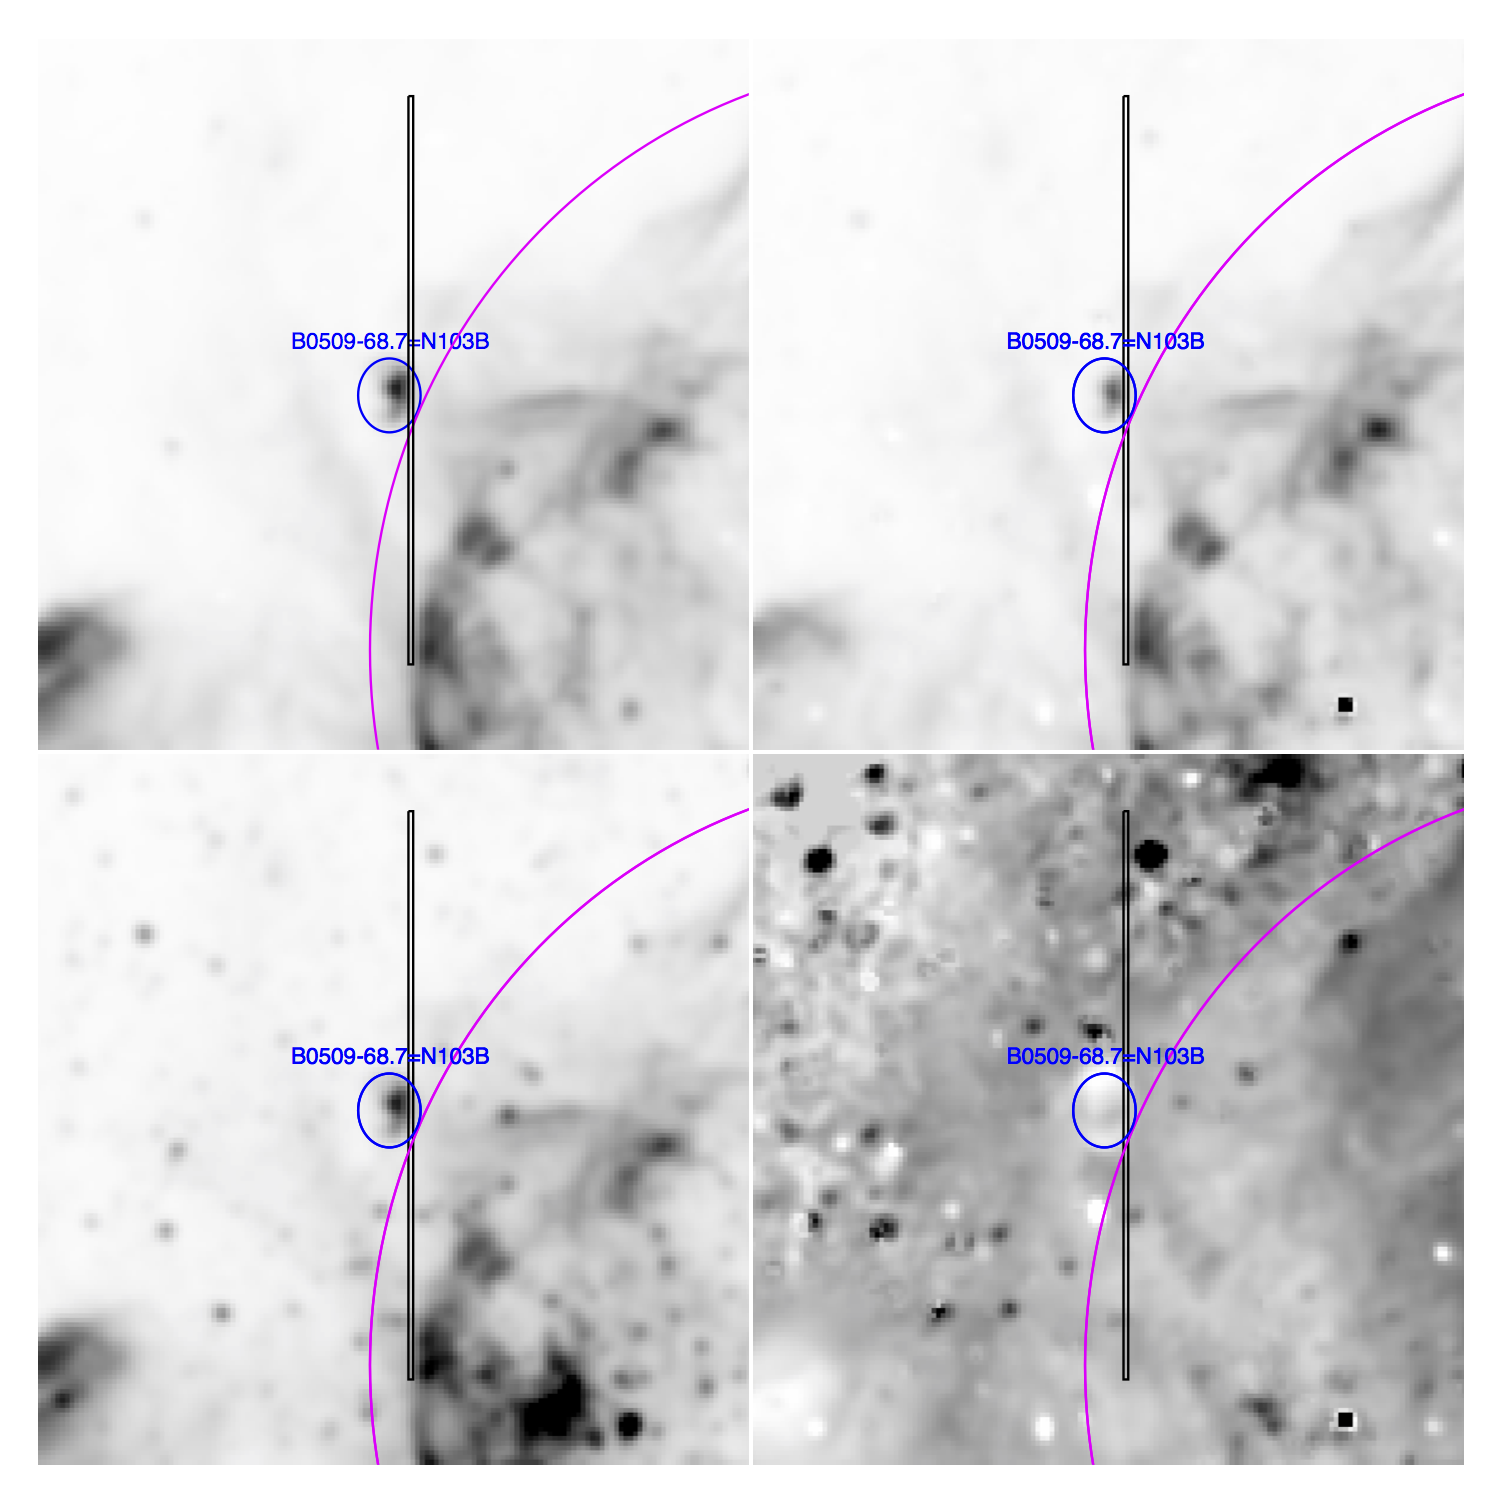
\includegraphics[width=10.05cm]{snapshots/N103B_5arcmin.png}
\end{figure}

\newpage
{\bf J509-6731 = B0509-67.5}  (Balmer-dominated; 5 arcmin field)
 
 ($v \approx 6700$ km/s per Hovey 2013, 2015)
 
Slit Center:   5:09:28.212   -67:31:07.856     N-S  

Scan:  East

Scan rate:  

Date/Frames:

Exposure Times:  

\begin{figure}
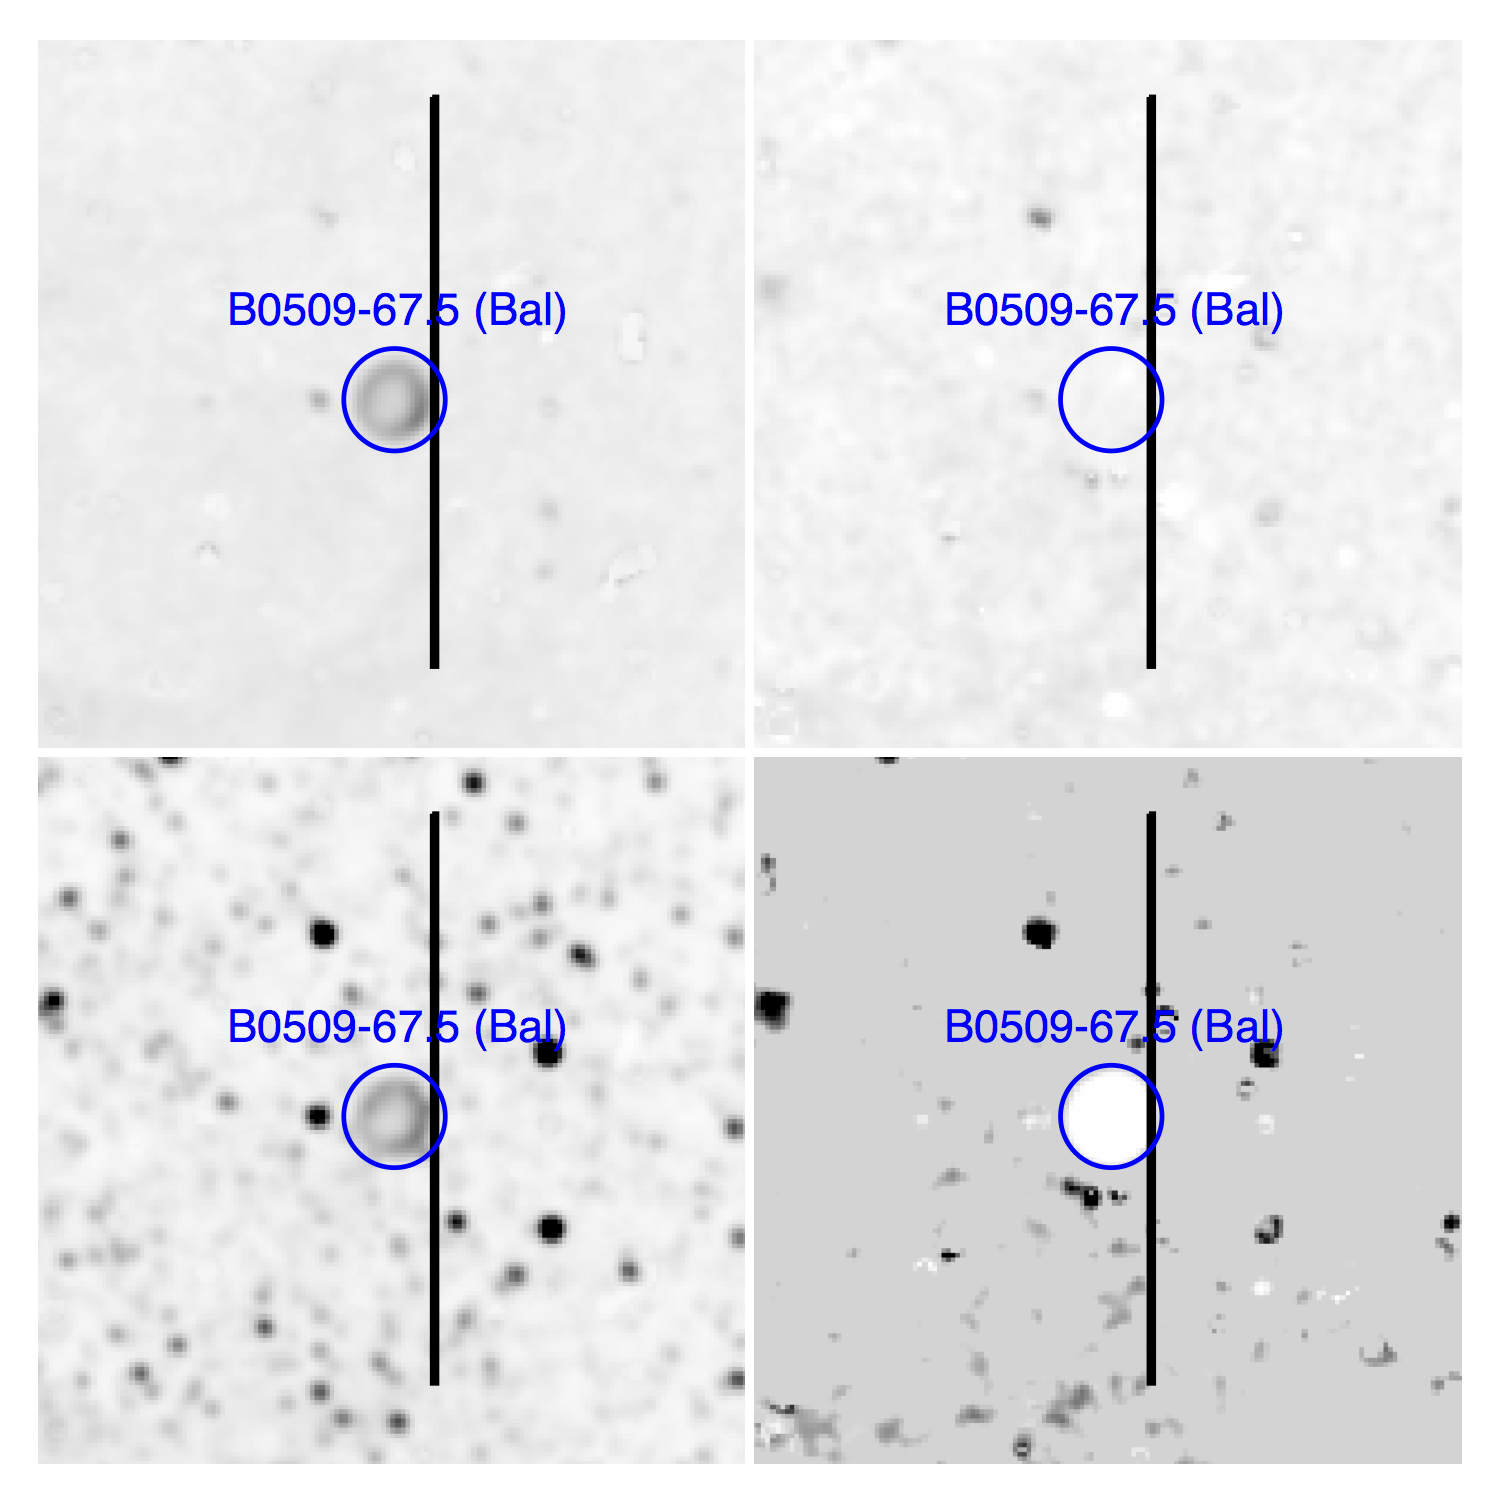
\includegraphics[width=10.05cm]{snapshots/B0509-675_5arcmin.png}
\end{figure}

\newpage
{\bf J0511-6759}  
 
Slit Center:   5:10:57.433   -67:59:01.202     N-S 

Scan:  East

Scan rate:  

Date/Frames:

Exposure Times:  

\begin{figure}
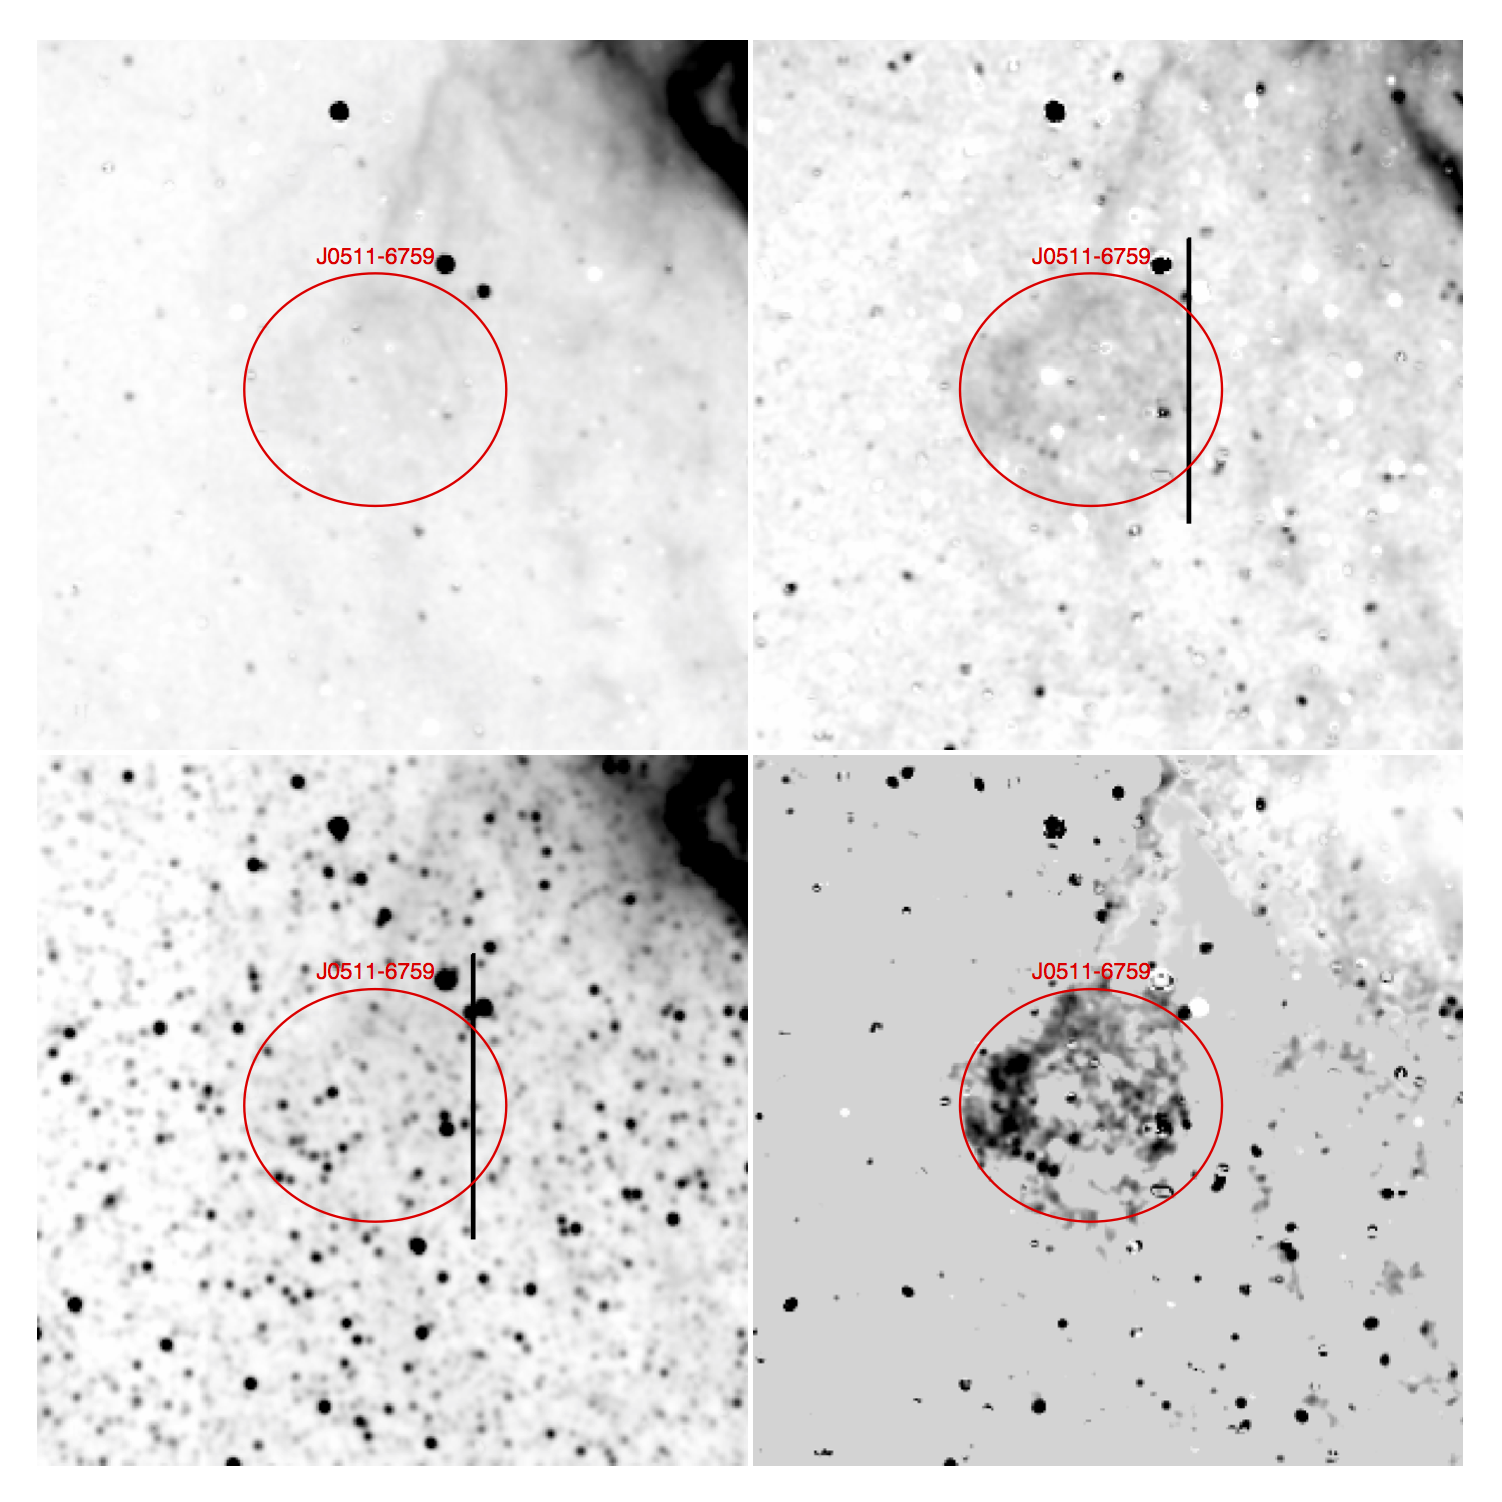
\includegraphics[width=10.05cm]{snapshots/J0511-6759.png}
\end{figure}

\newpage
{\bf J0512-6707}  
 
Slit Center:   5:12:25.064  -67:07:04.034    N-S 

Scan:  East

Scan rate:  

Date/Frames:

Exposure Times:  

\begin{figure}
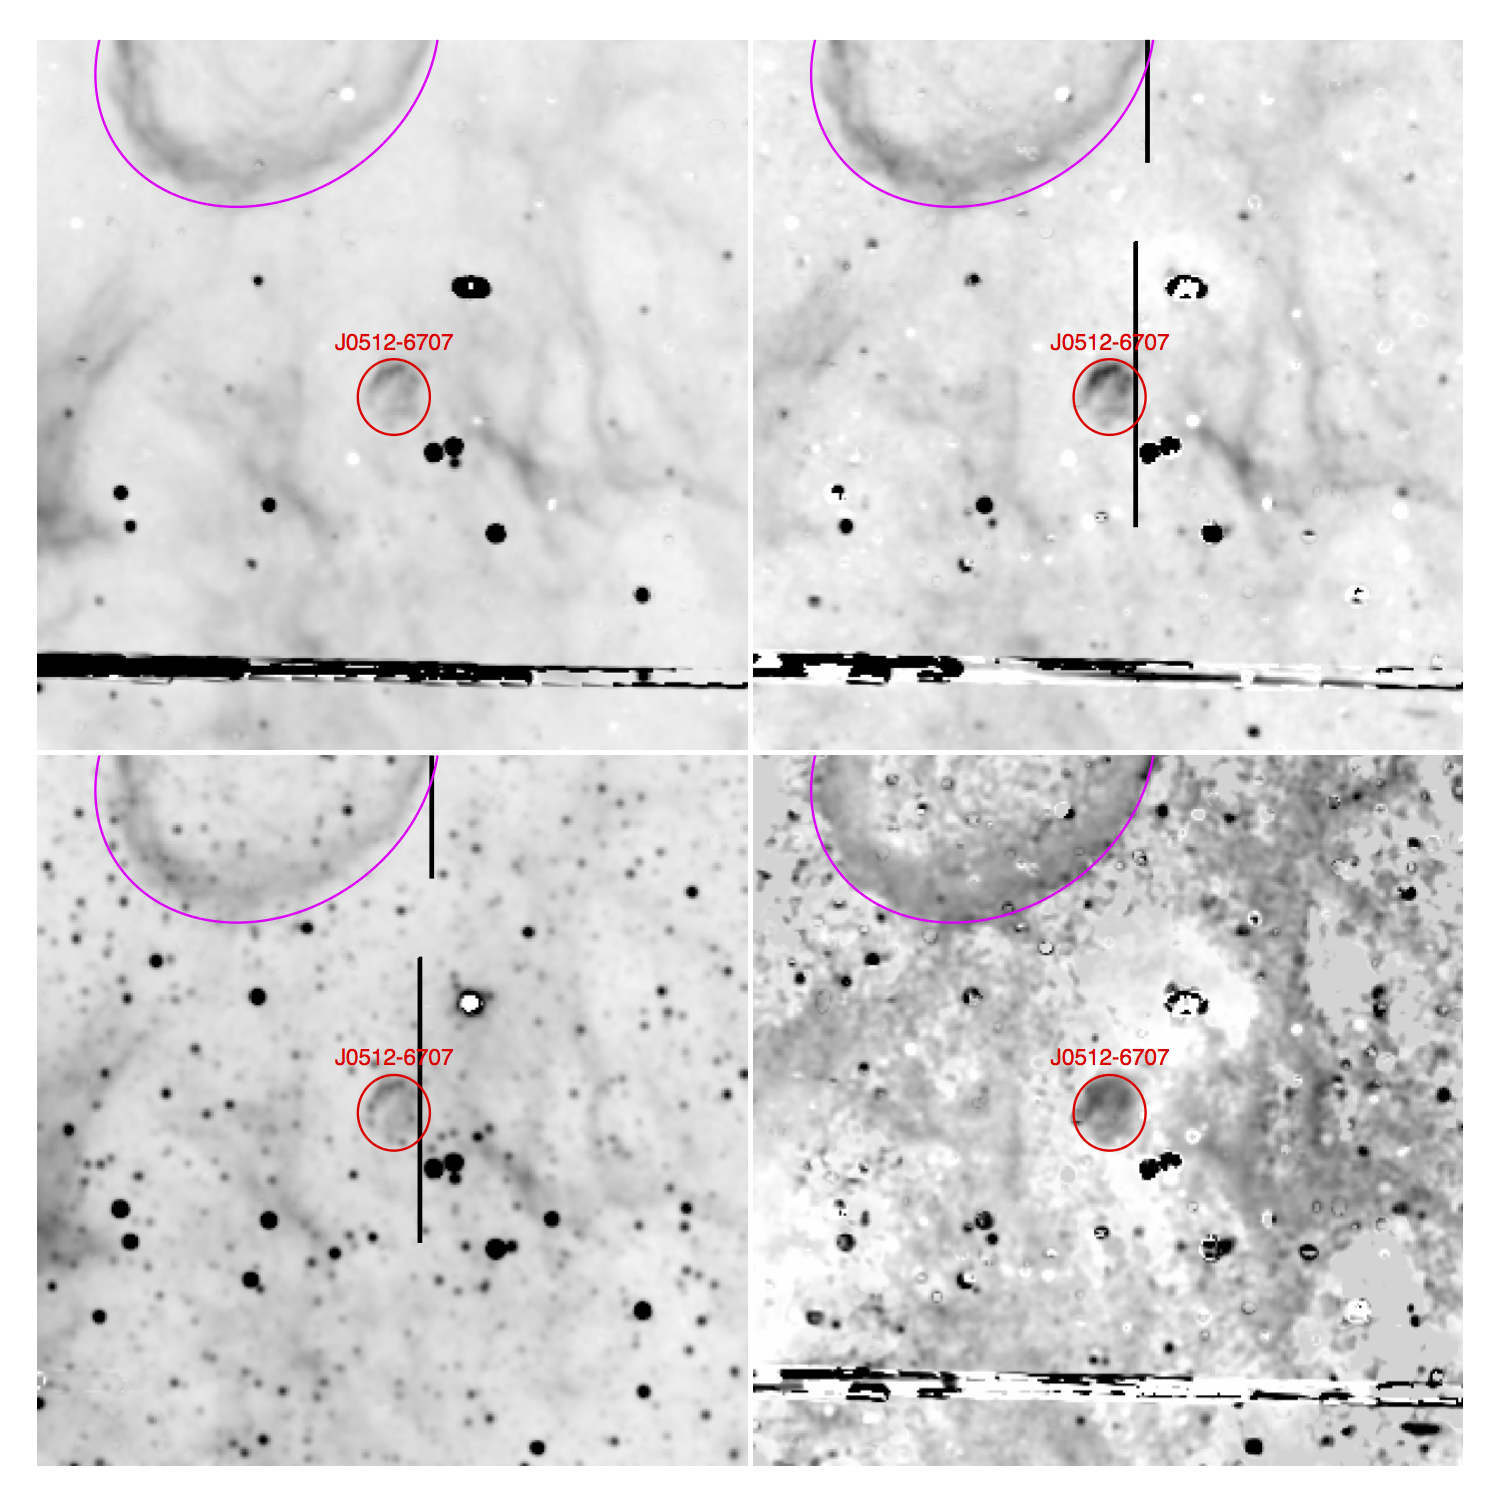
\includegraphics[width=10.05cm]{snapshots/J0512-6707.png}
\end{figure}

\newpage
{\bf J0512-6702 (new)}  
 
Slit Center:   5:10:57.433   -67:59:01.202    N-S 

Scan:  East

Scan rate:  

Date/Frames:

Exposure Times:  

\begin{figure}
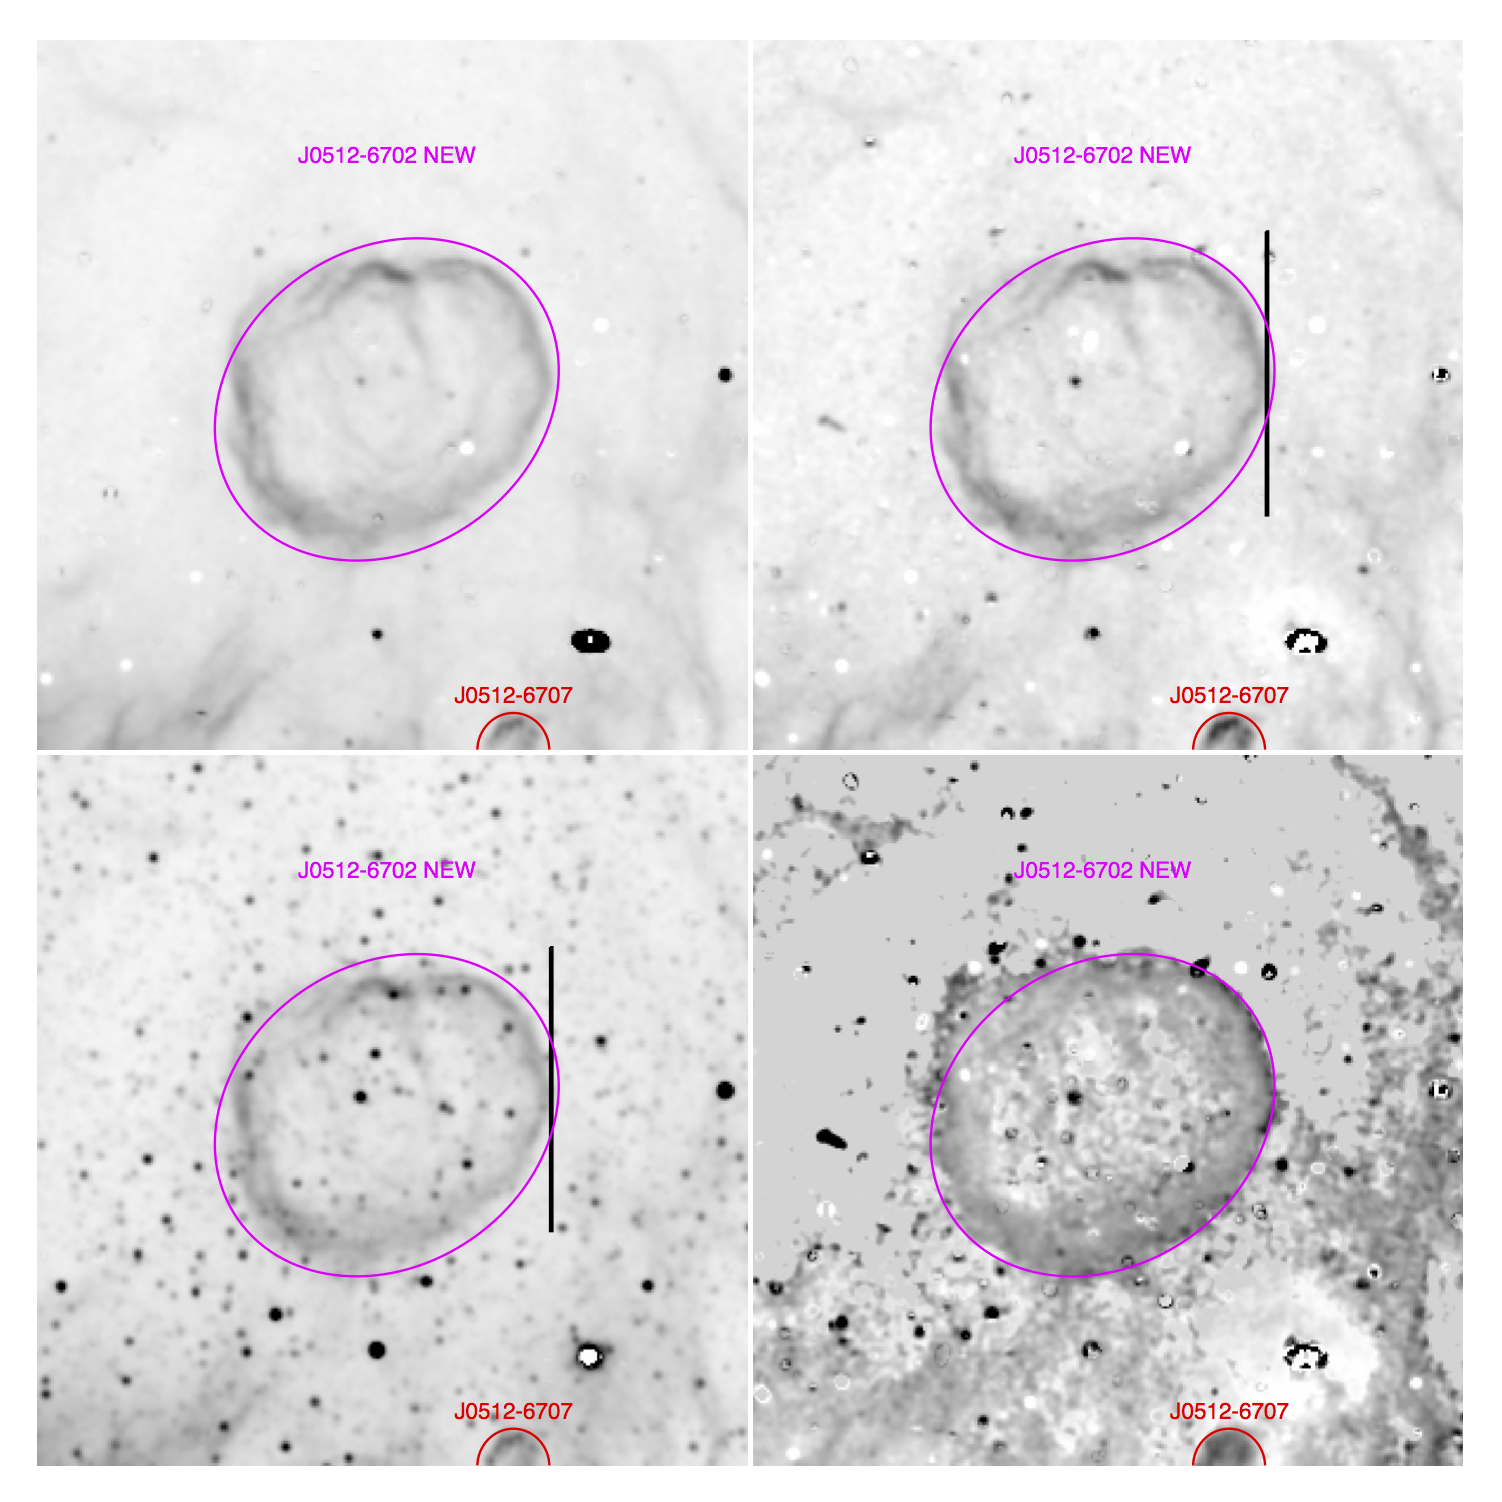
\includegraphics[width=10.05cm]{snapshots/J0512-6702.png}
\end{figure}

\newpage
{\bf J0513-6912-6912 = B0513-69.2}  
 
Slit Center:   5:12:53.465, -69:12:15.860    N-S 

Scan:  East

Scan rate:  

Date/Frames:

Exposure Times:  

\begin{figure}
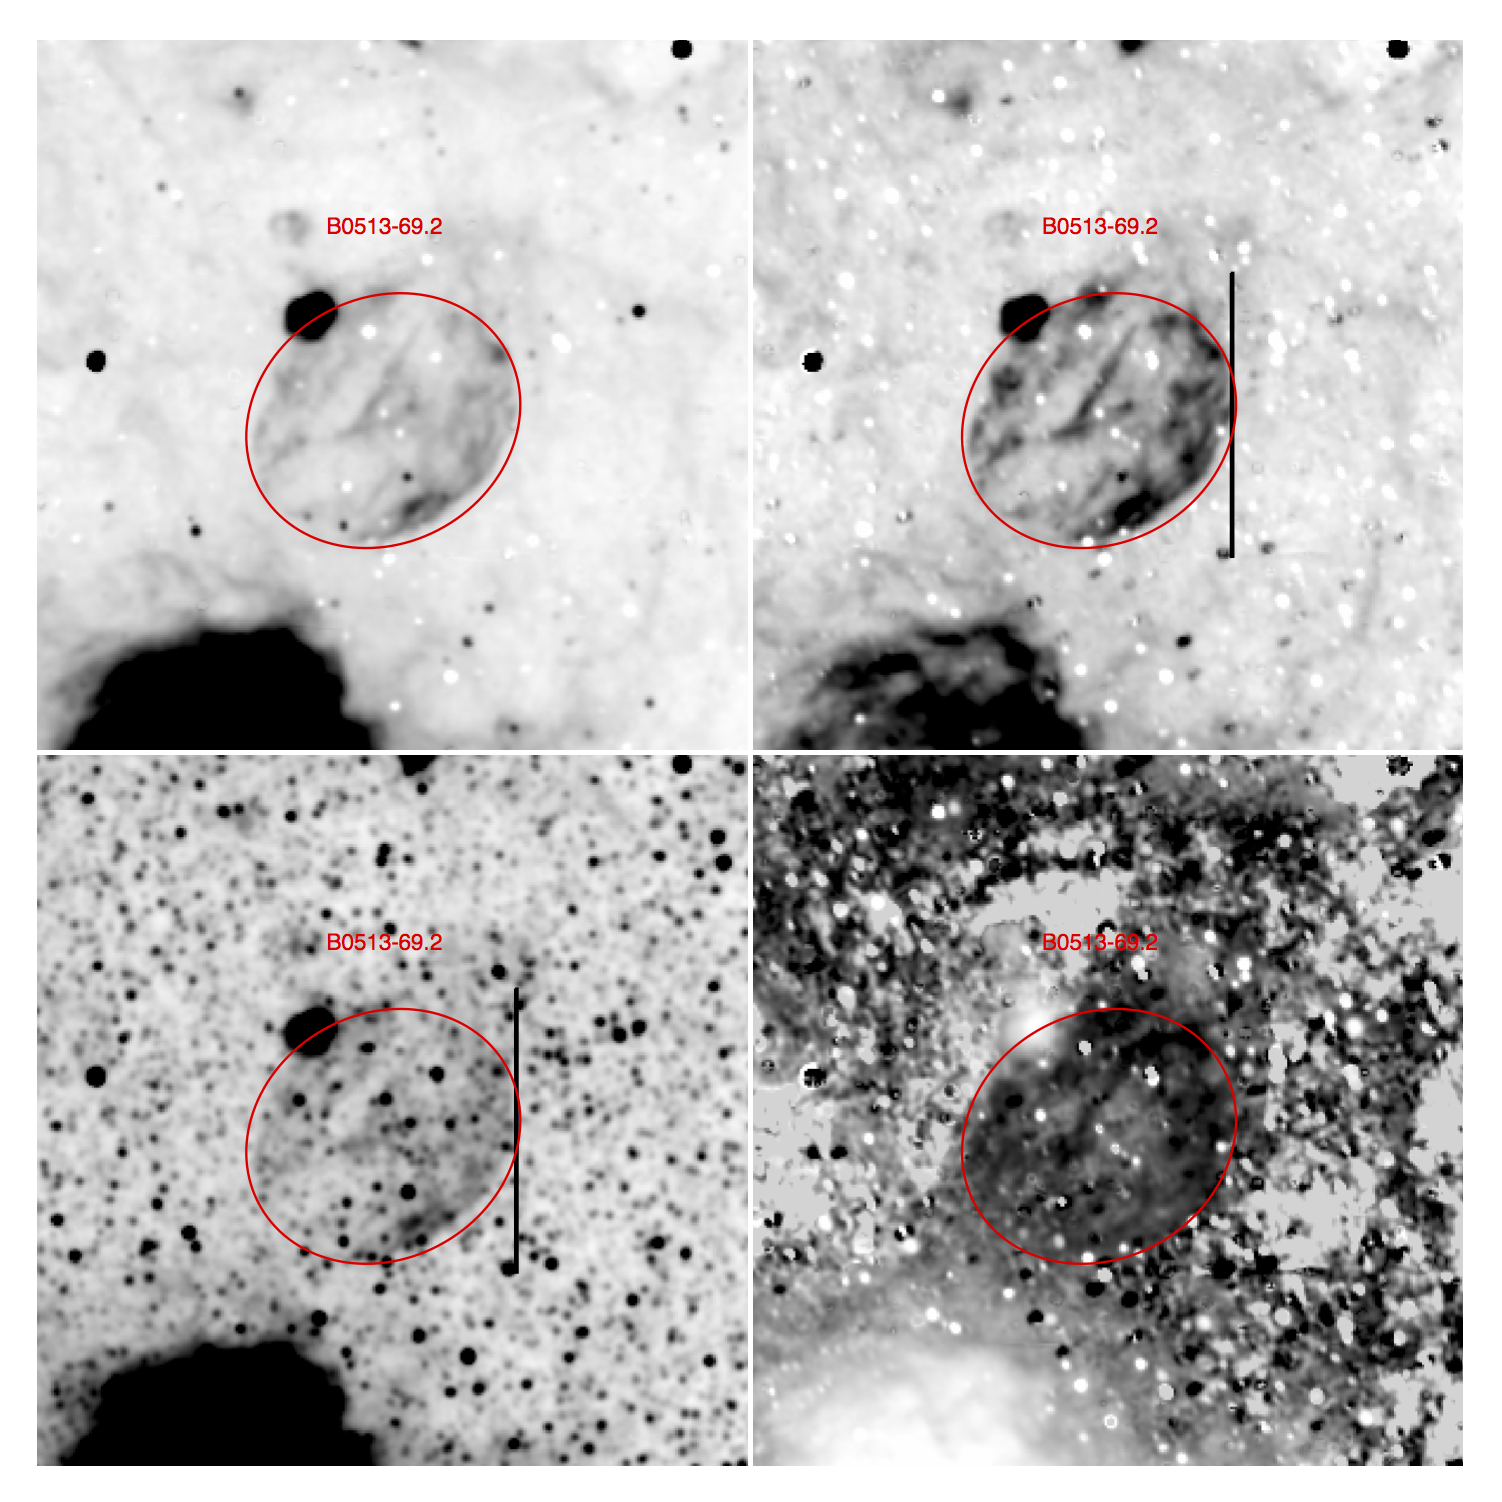
\includegraphics[width=10.05cm]{snapshots/B0513-692.png}
\end{figure}

\newpage
{\bf J0514-6840}  
 
Slit Center:   5:14:01.698 -68:40:53.008    N-S 

Scan:  East

Scan rate:  

Date/Frames:

Exposure Times:  

\begin{figure}
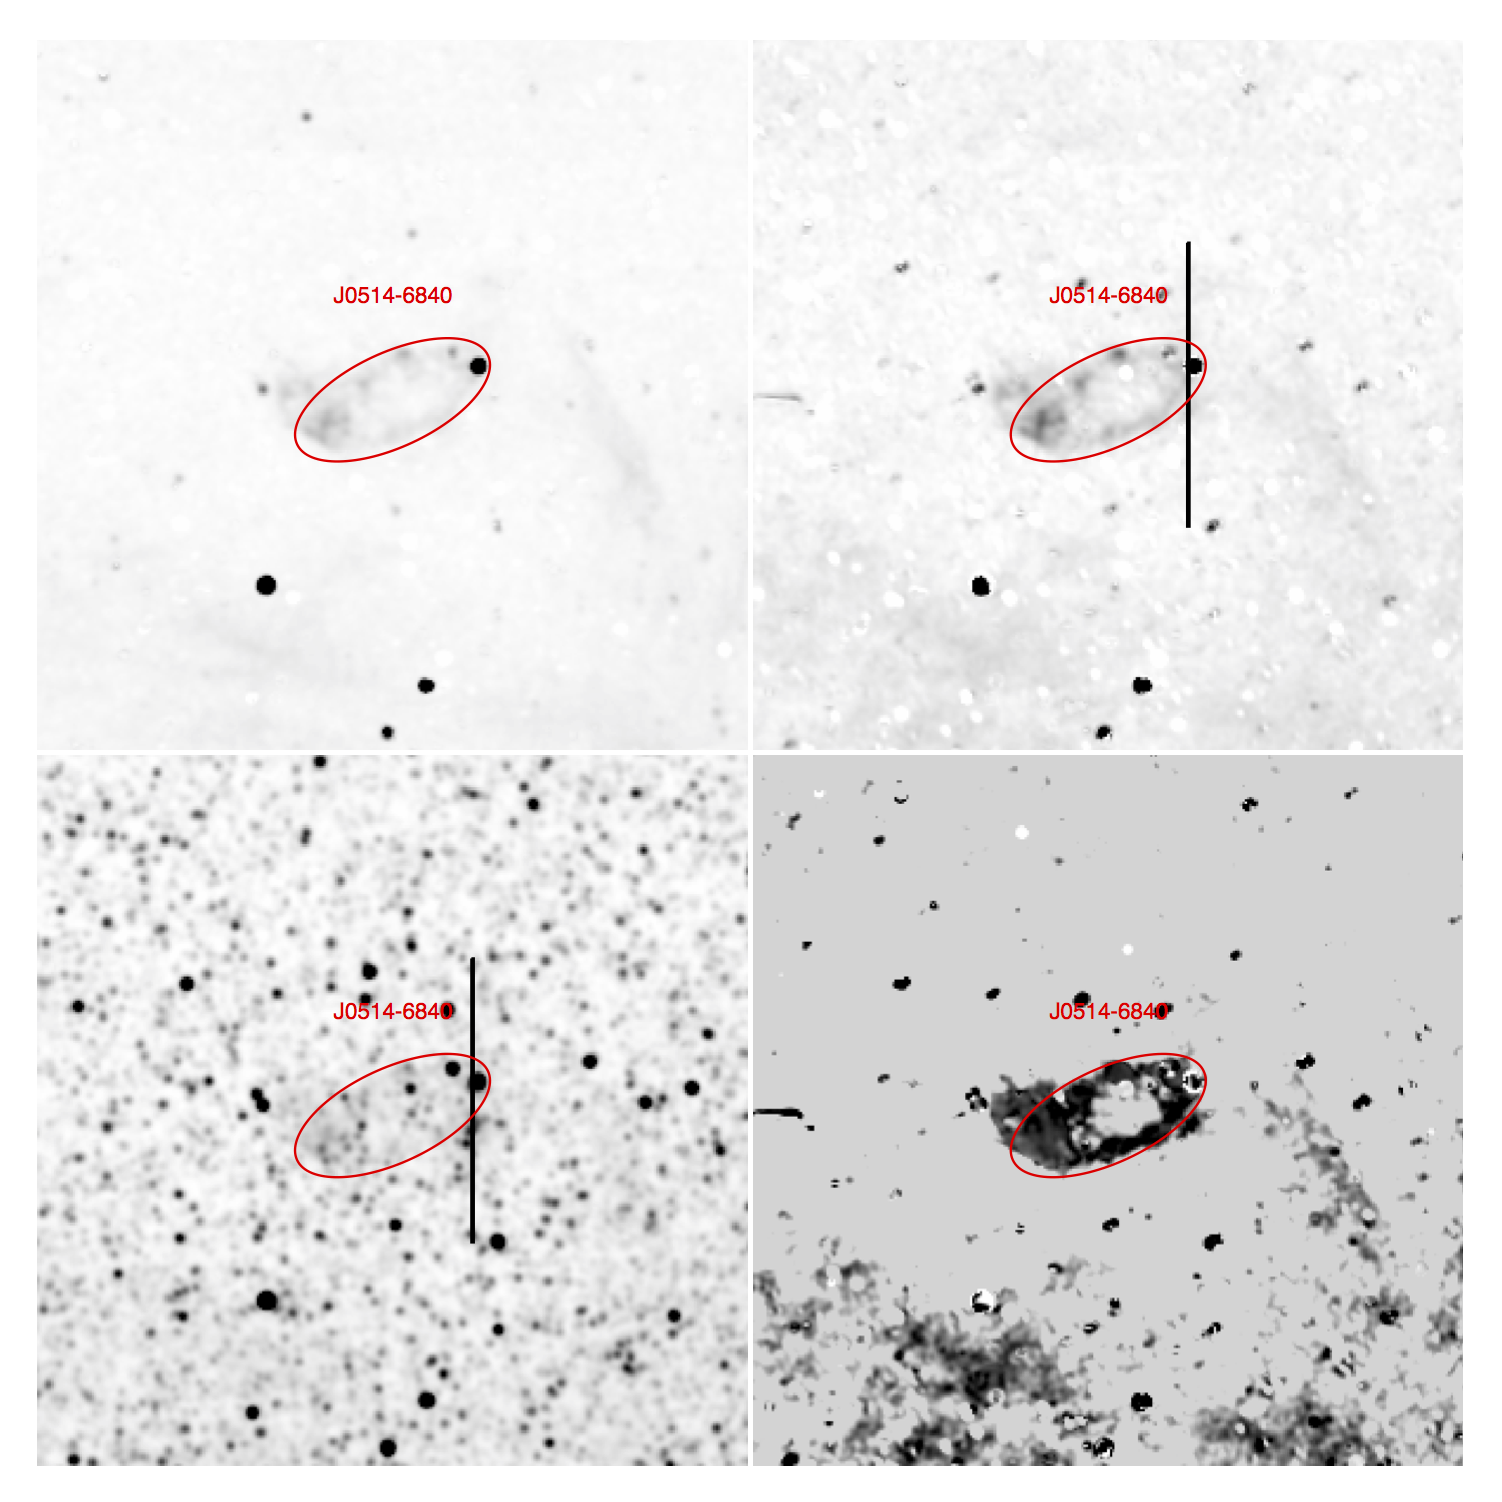
\includegraphics[width=10.05cm]{snapshots/J0514-6840.png}
\end{figure}

\newpage
{\bf J0517-6759}  
 
Slit Center:   5:17:07.268 -68:01:28.513    E-W 

Scan:  North

Scan rate:  

Date/Frames:

Exposure Times:  

\begin{figure}
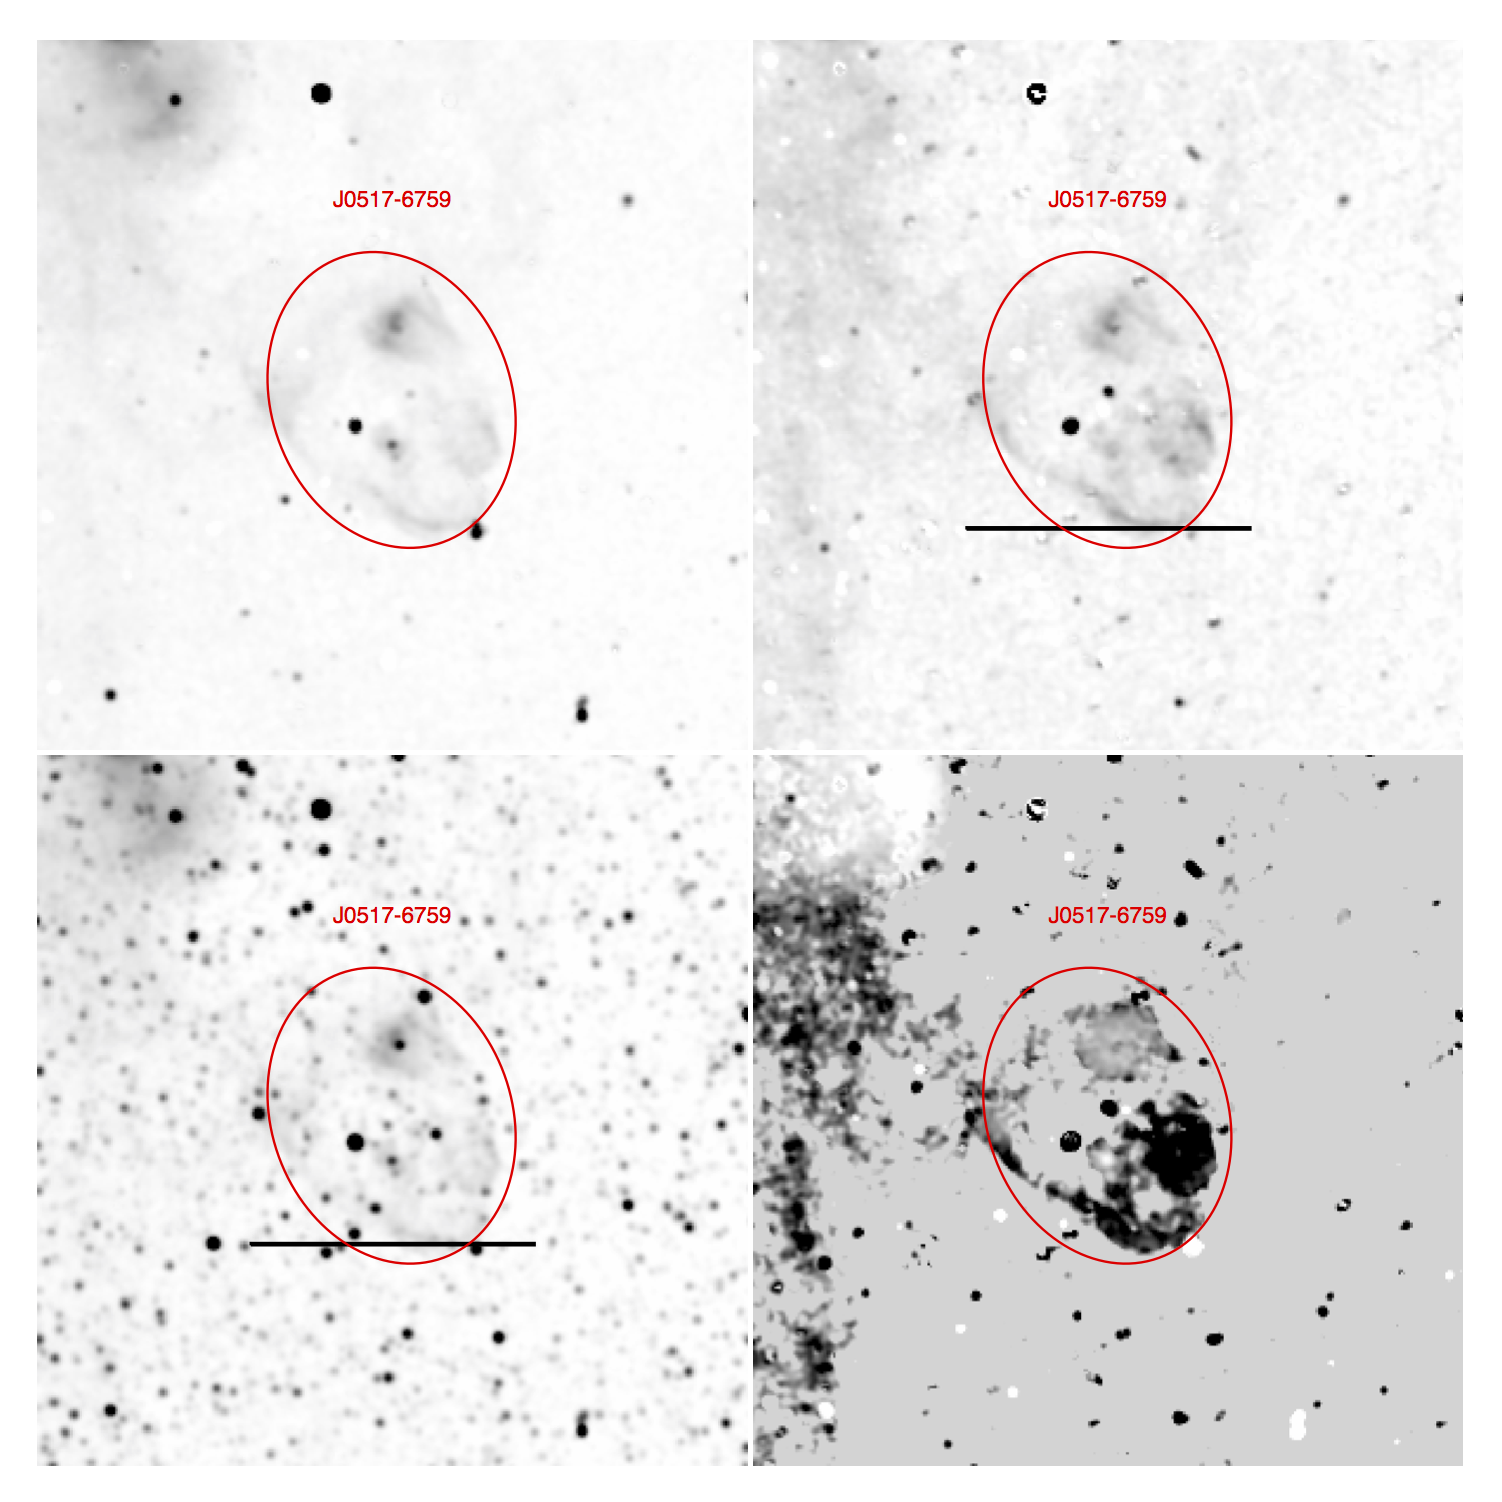
\includegraphics[width=10.05cm]{snapshots/J0517-6759.png}
\end{figure}

\newpage
{\bf J0518-6939 = B0519-69.7 = N120}  
 
Slit Center:   5:18:36.899  -69:39:06.699   N-S

Scan:  East

Scan rate:  

Date/Frames:

Exposure Times:  

May be hard; lots of background
\begin{figure}
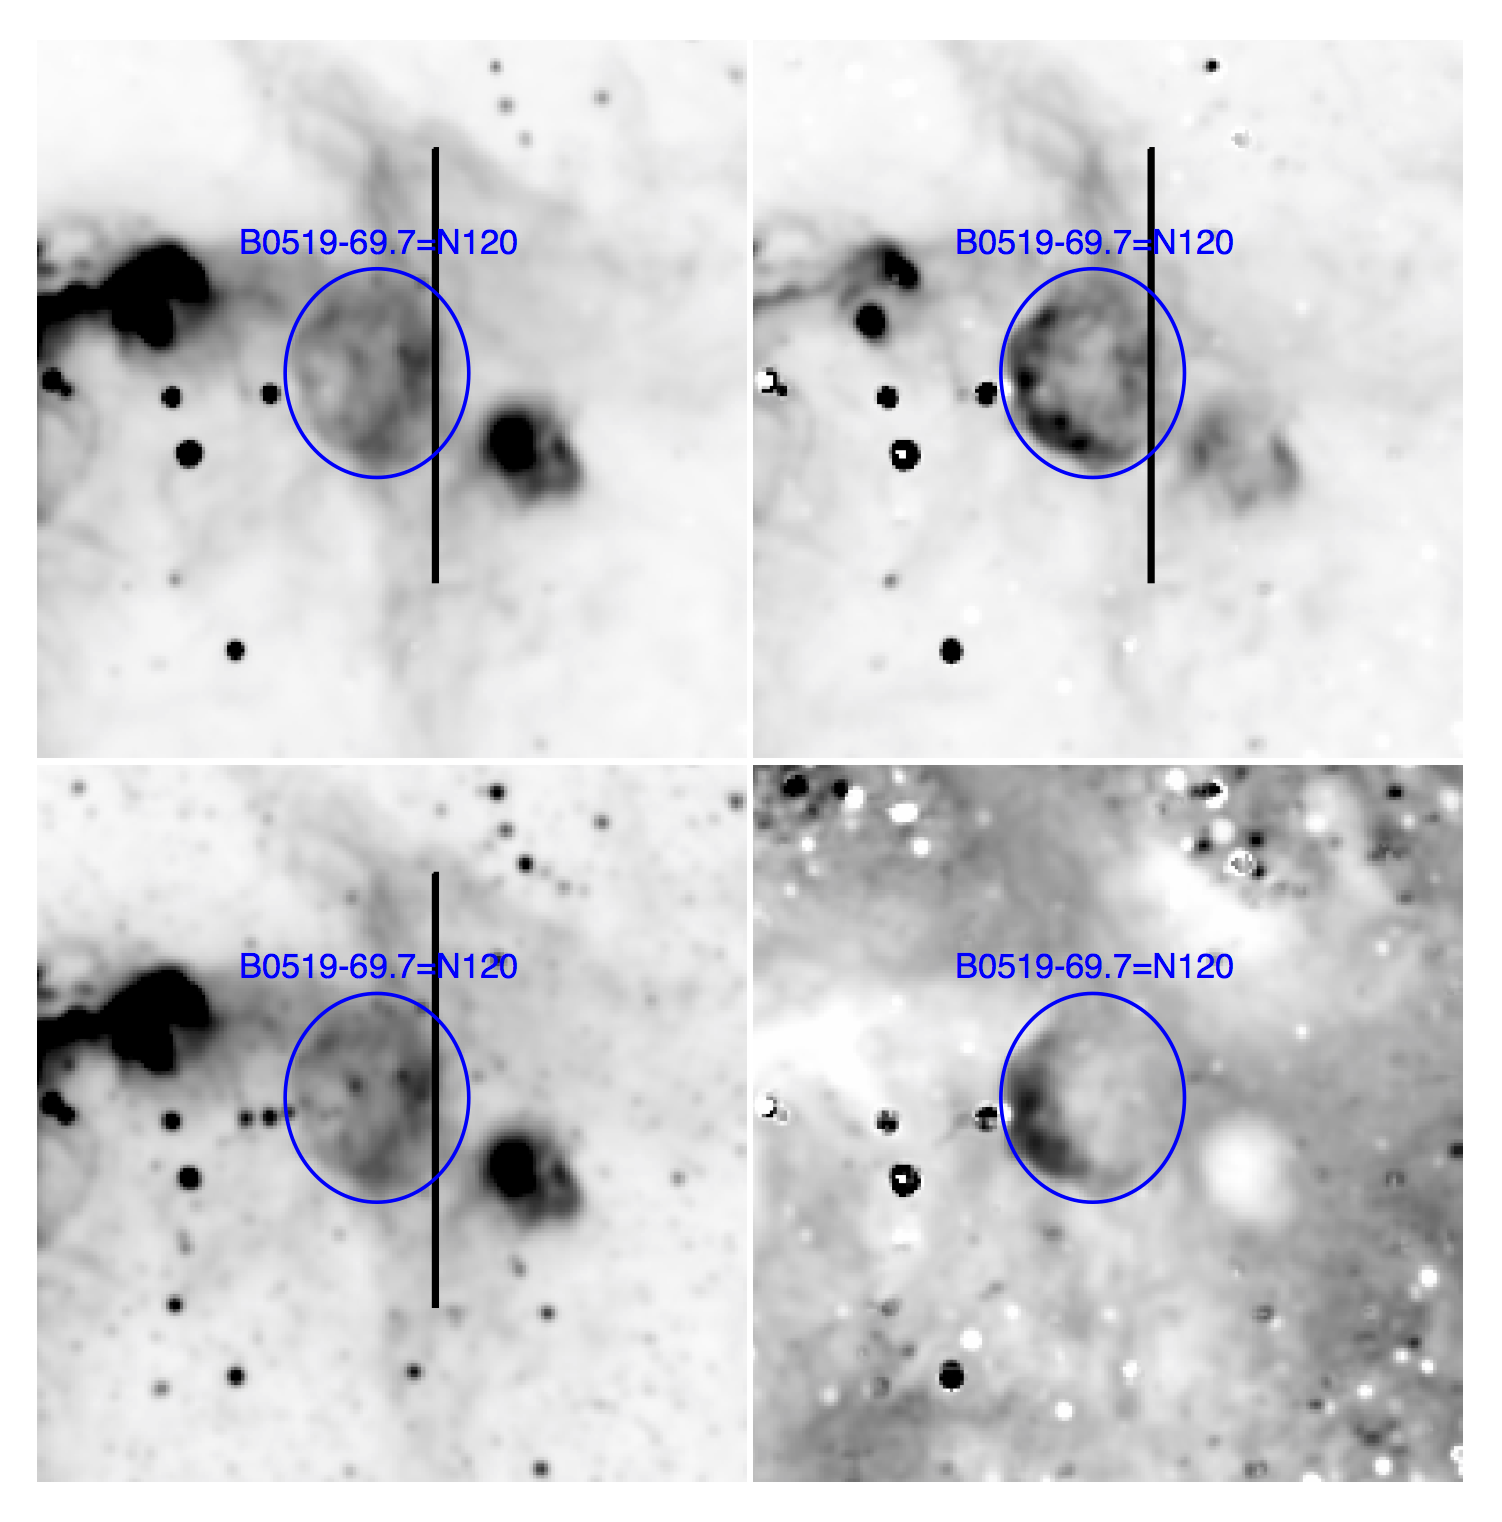
\includegraphics[width=10.05cm]{snapshots/B0519-697.png}
\end{figure}

\newpage
{\bf J0519--6902 = B0519-69.0 (Balmer-dominated; 5 arcmin field)}  
 
Slit Center:   5:19:31.401,-69:02:16.171 N-S

Scan:  East

Scan rate:  

Date/Frames:

Exposure Times:  

\begin{figure}
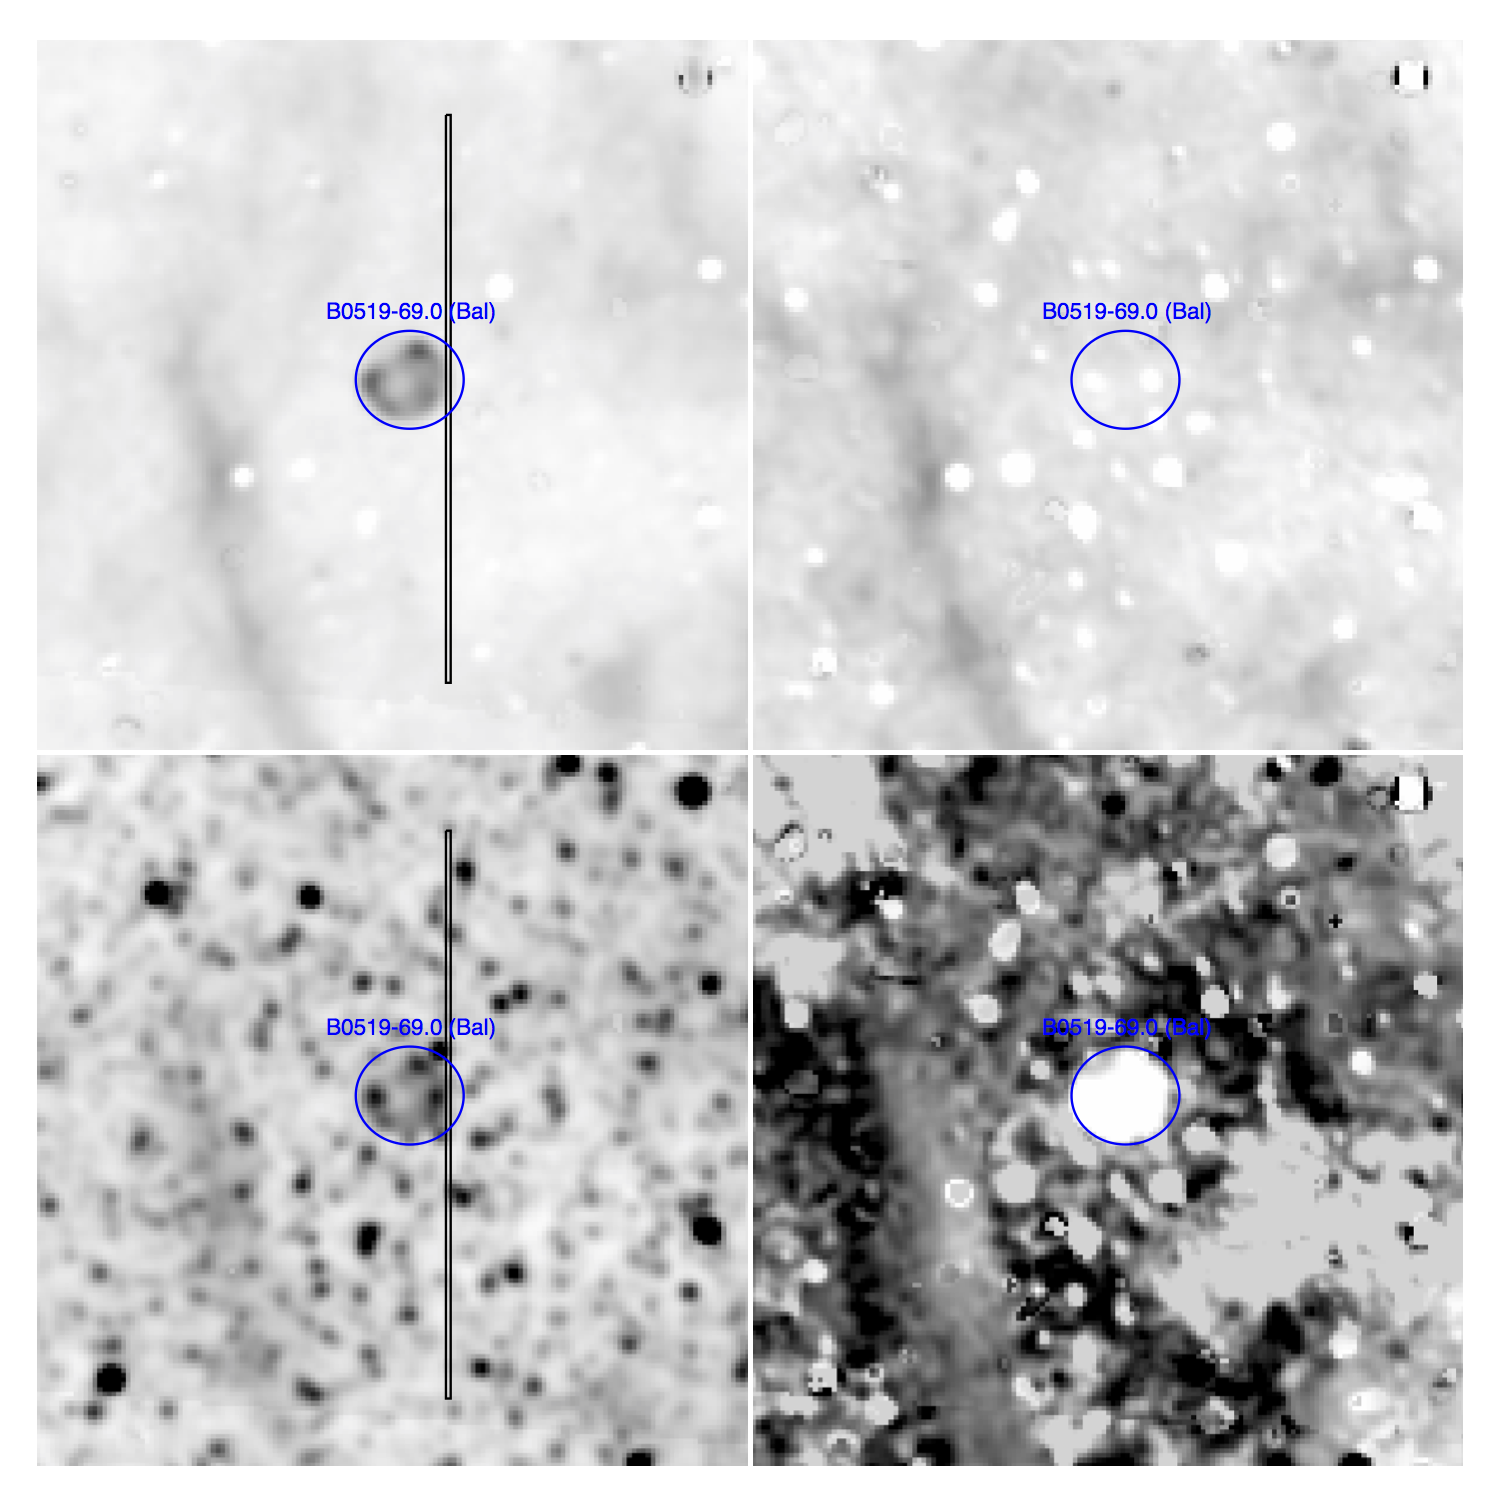
\includegraphics[width=10.05cm]{snapshots/B0519-690_5arcmin.png}
\end{figure}

\newpage
{\bf J0519--6925 = B0520-69.4}  
 
Slit Center:   5:19:33.637  -69:25:56.631 N-S

Scan:  East

Scan rate:  

Date/Frames:

Exposure Times:  

\begin{figure}
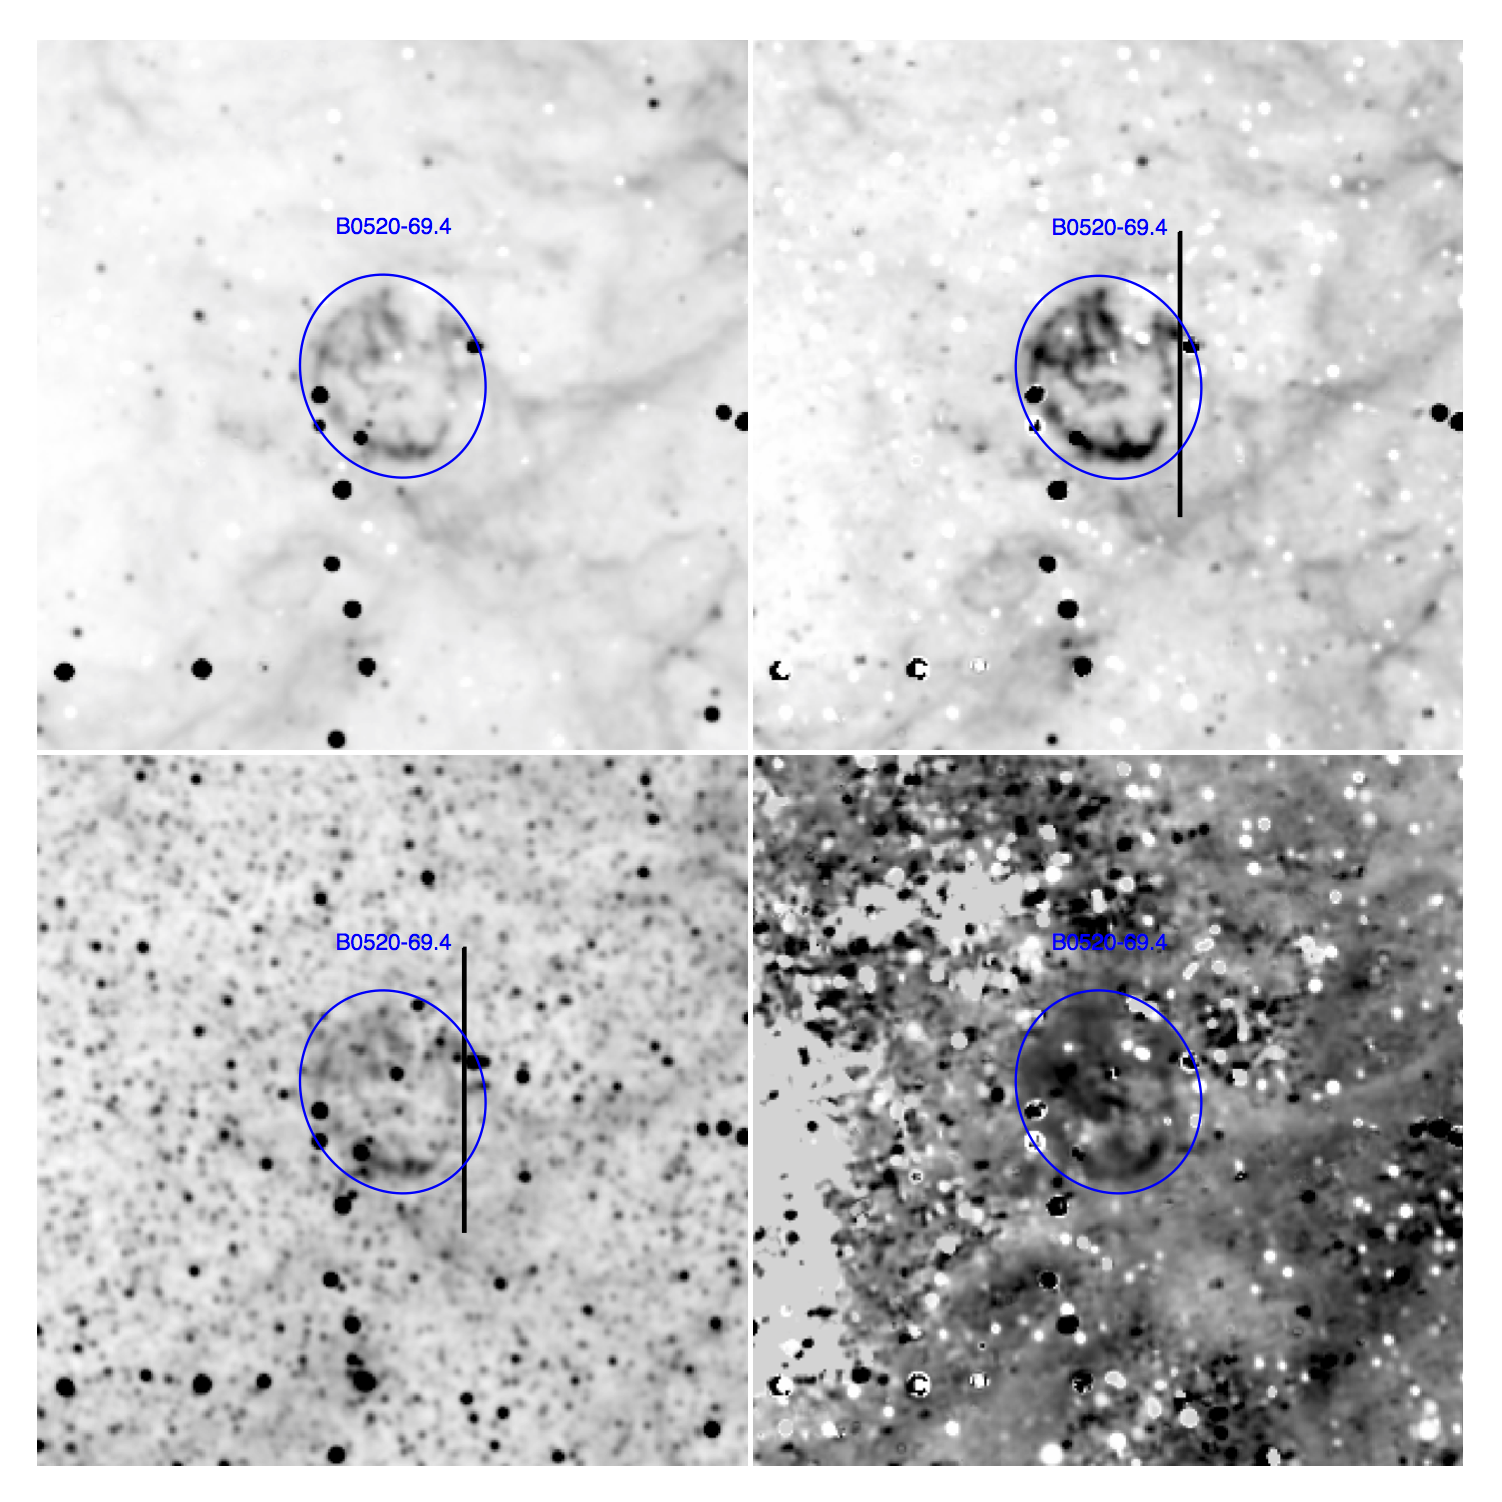
\includegraphics[width=10.05cm]{snapshots/B0520-694.png}
\end{figure}

\newpage
{\bf J0521-6542 = DEML142}  
 
Slit Center:   5:21:26.390   -65:43:10.137   N-S

Scan:  East

Scan rate:  

Date/Frames:

Exposure Times:  

\begin{figure}
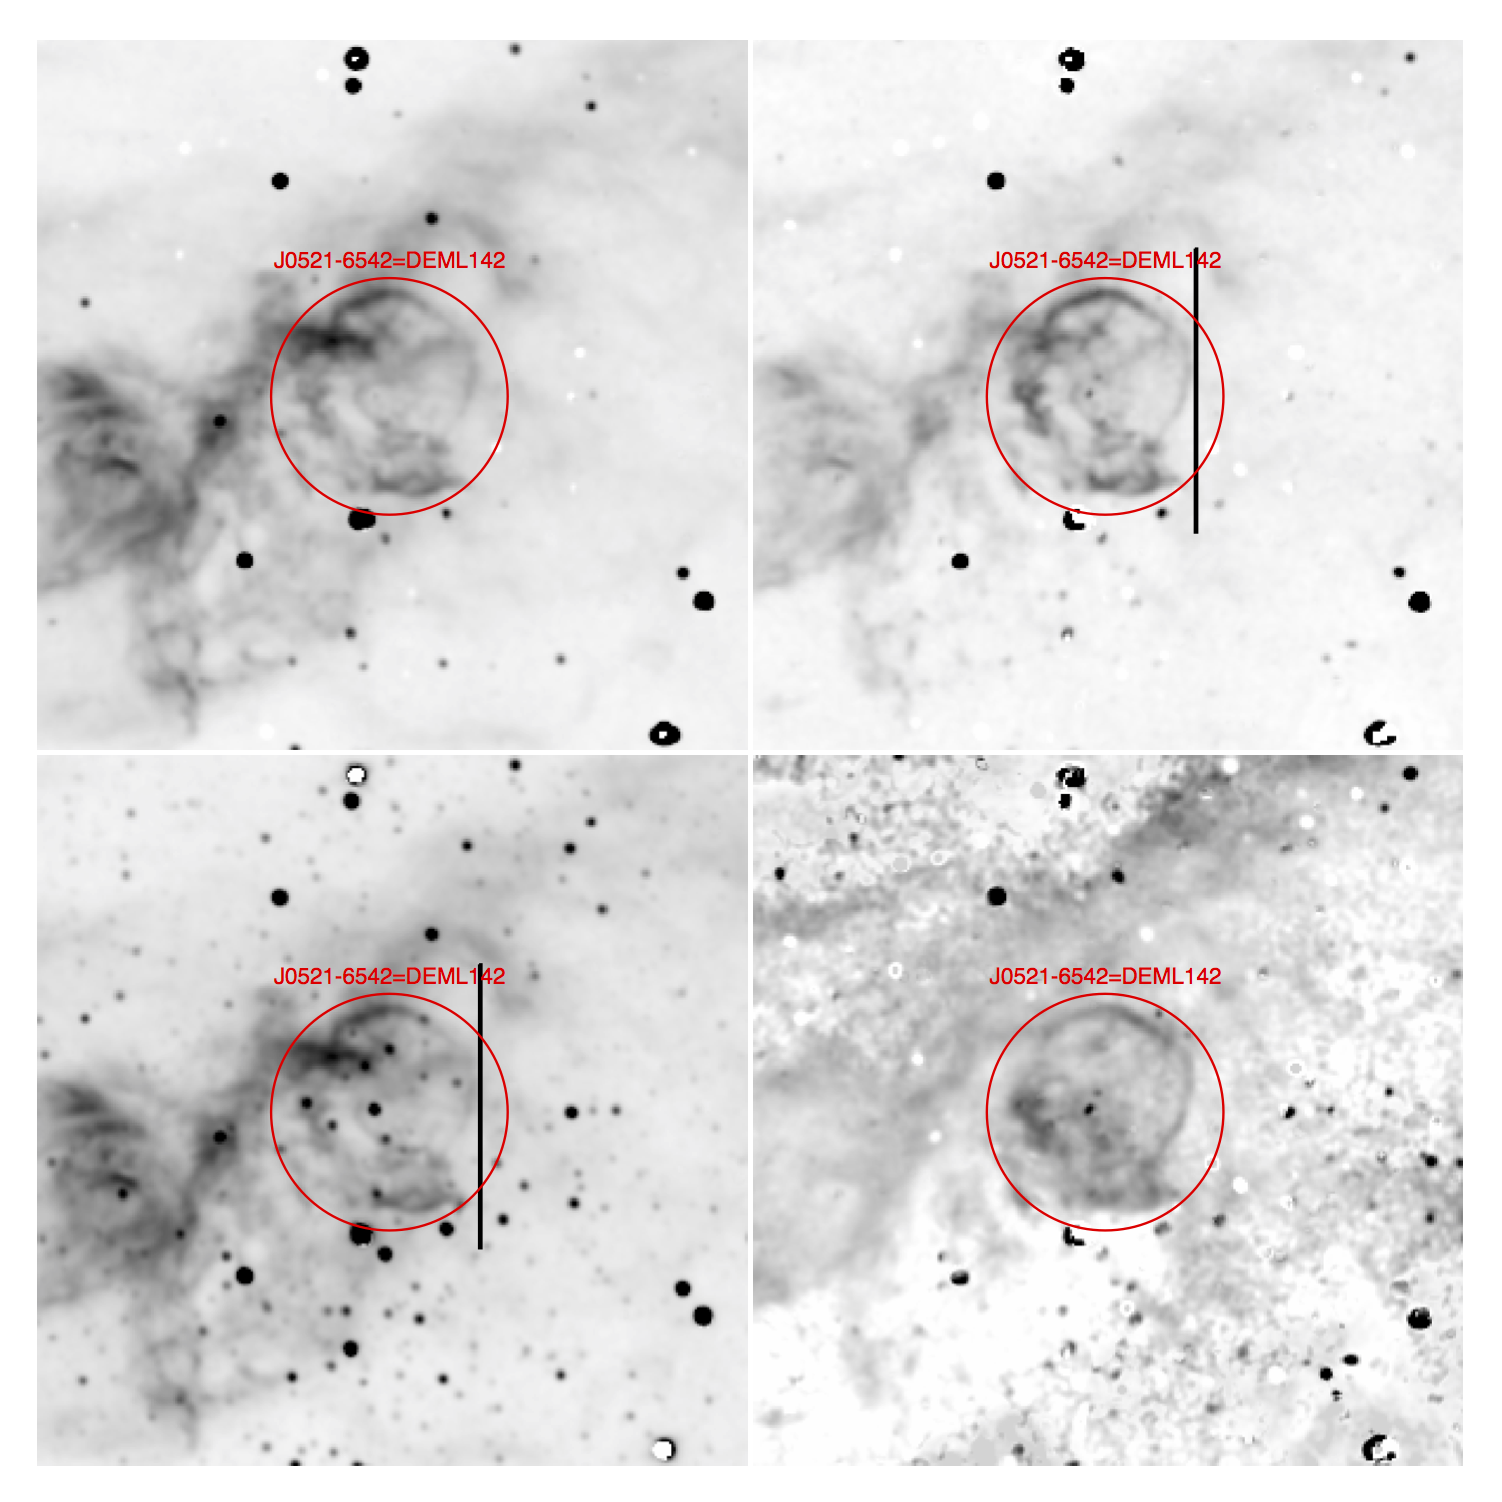
\includegraphics[width=10.05cm]{snapshots/J0521-6542.png}
\end{figure}

\newpage
{\bf J0523-6753 = N441}  
 
Slit Center:   5:22:42.636  -67:53:09.888 N-S

Scan:  East

Scan rate:  

Date/Frames:

Exposure Times:  

\begin{figure}
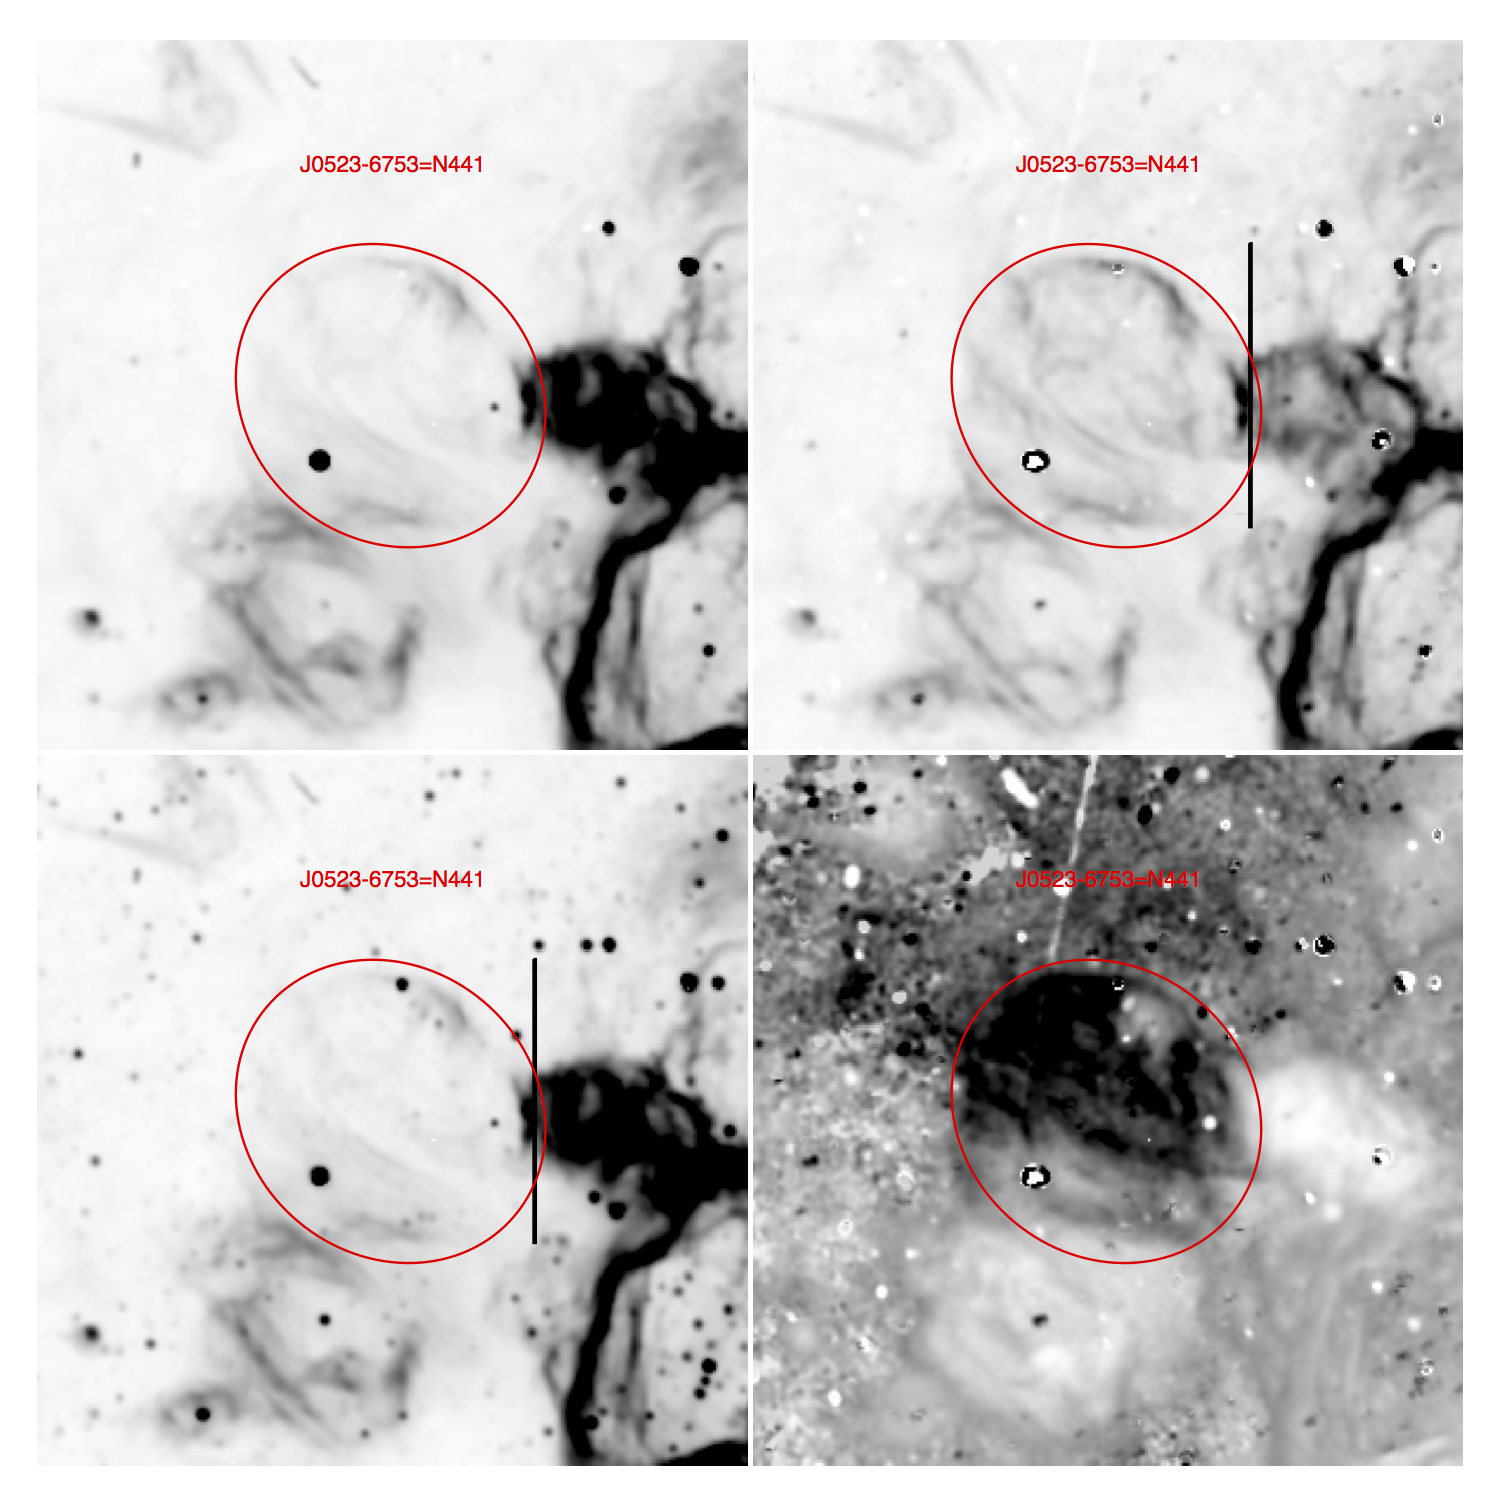
\includegraphics[width=10.05cm]{snapshots/J0523-6753.png}
\end{figure}

\newpage
{\bf J0524-6623 = B0524-66.4}  
 
Slit Center:   5:24:05.457   -66:23:39.150 N-S

Scan:  East

Scan rate:  

Date/Frames:

Exposure Times:  

\begin{figure}
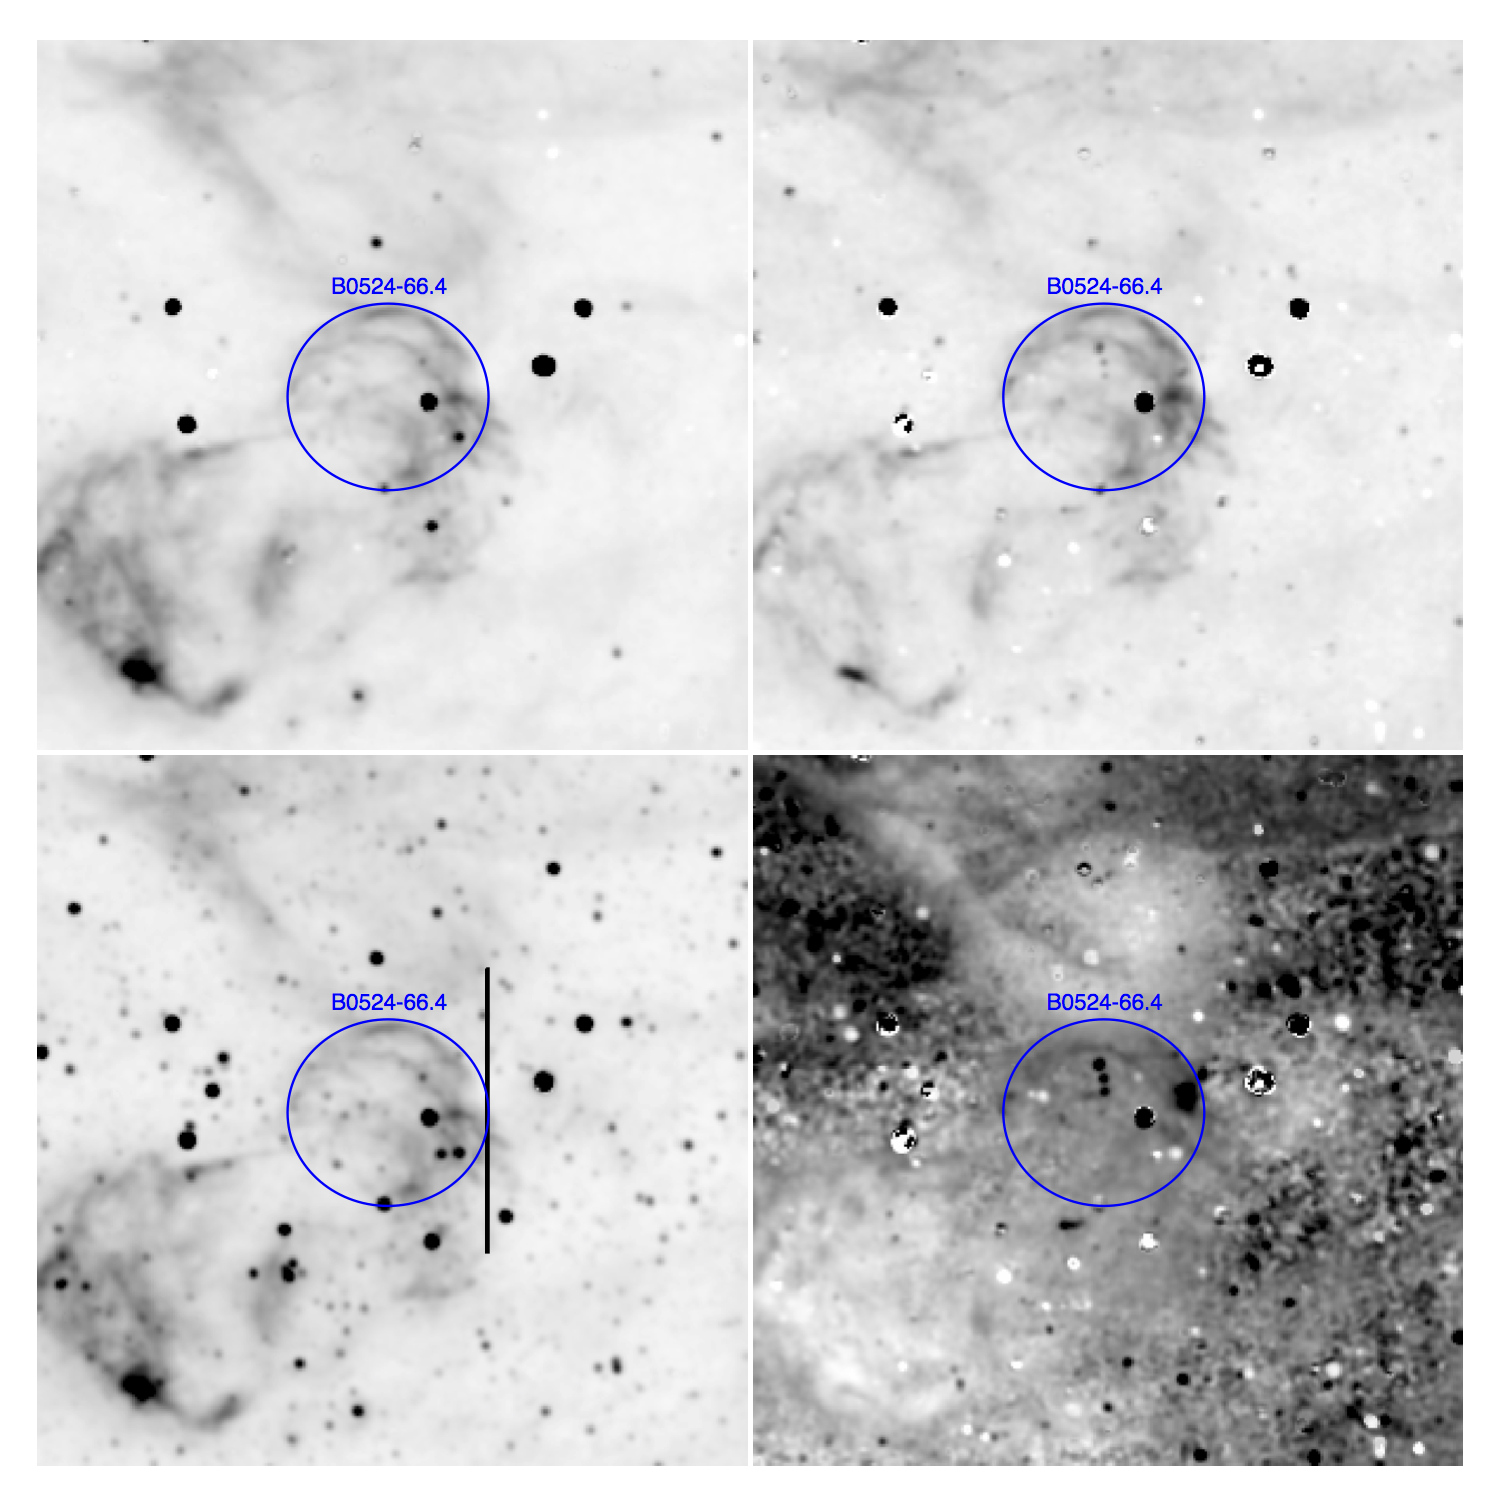
\includegraphics[width=10.05cm]{snapshots/B0524-664.png}
\end{figure}

\newpage
{\bf J0525=6938 = N132D = B0525-69.6 (O-rich central region)}  
 
Slit Center:   5:24:52.055   -69:38:29.240 N-S

Scan:  East

Scan rate:  

Date/Frames:

Exposure Times:  

\begin{figure}
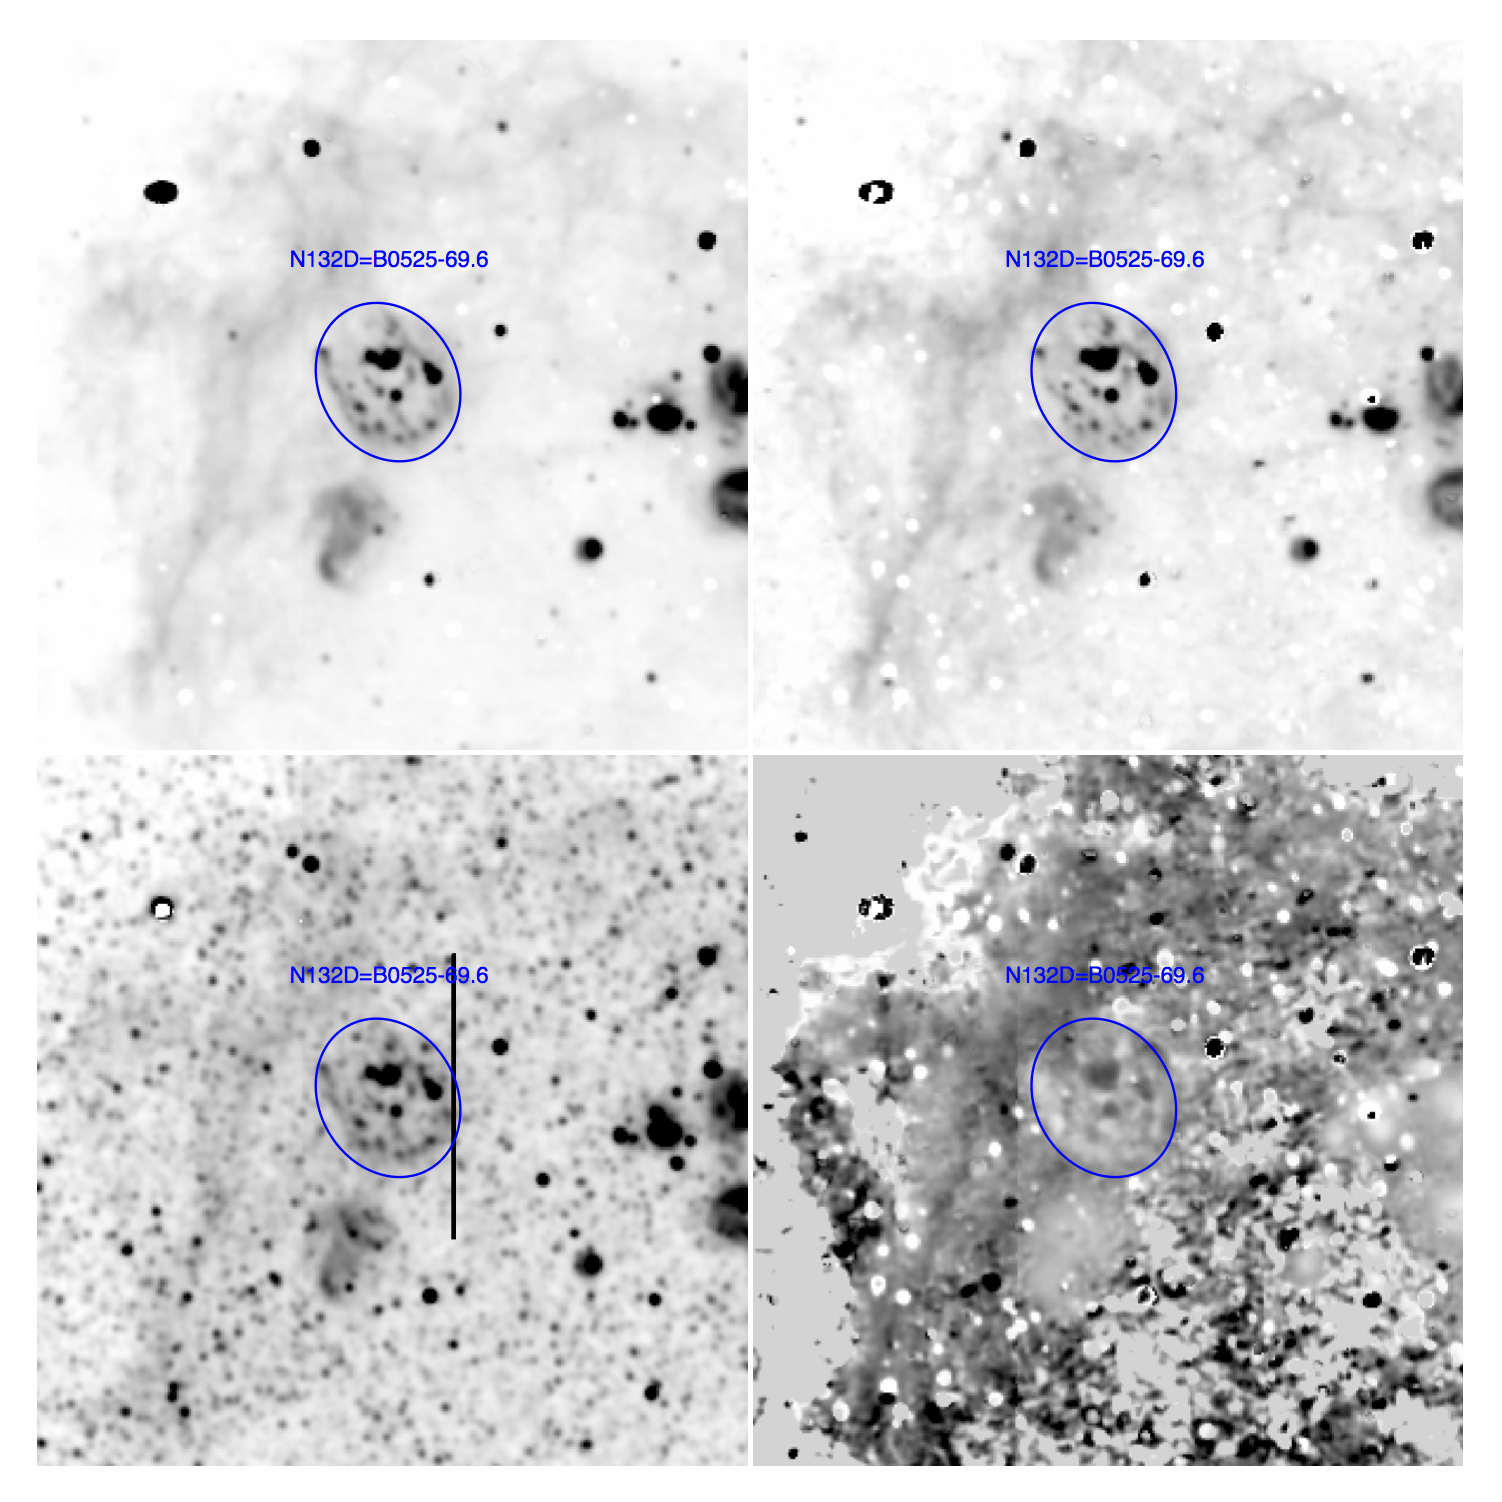
\includegraphics[width=10.05cm]{snapshots/N132D.png}
\end{figure}

\newpage
{\bf J0525=6559 = N49B = B0525-66.0 (5 arcmin field)}  
 
Slit Center:   5:25:27.359   -65:59:16.897 N-S

Scan:  East

Scan rate:  

Date/Frames:

Exposure Times:  

\begin{figure}
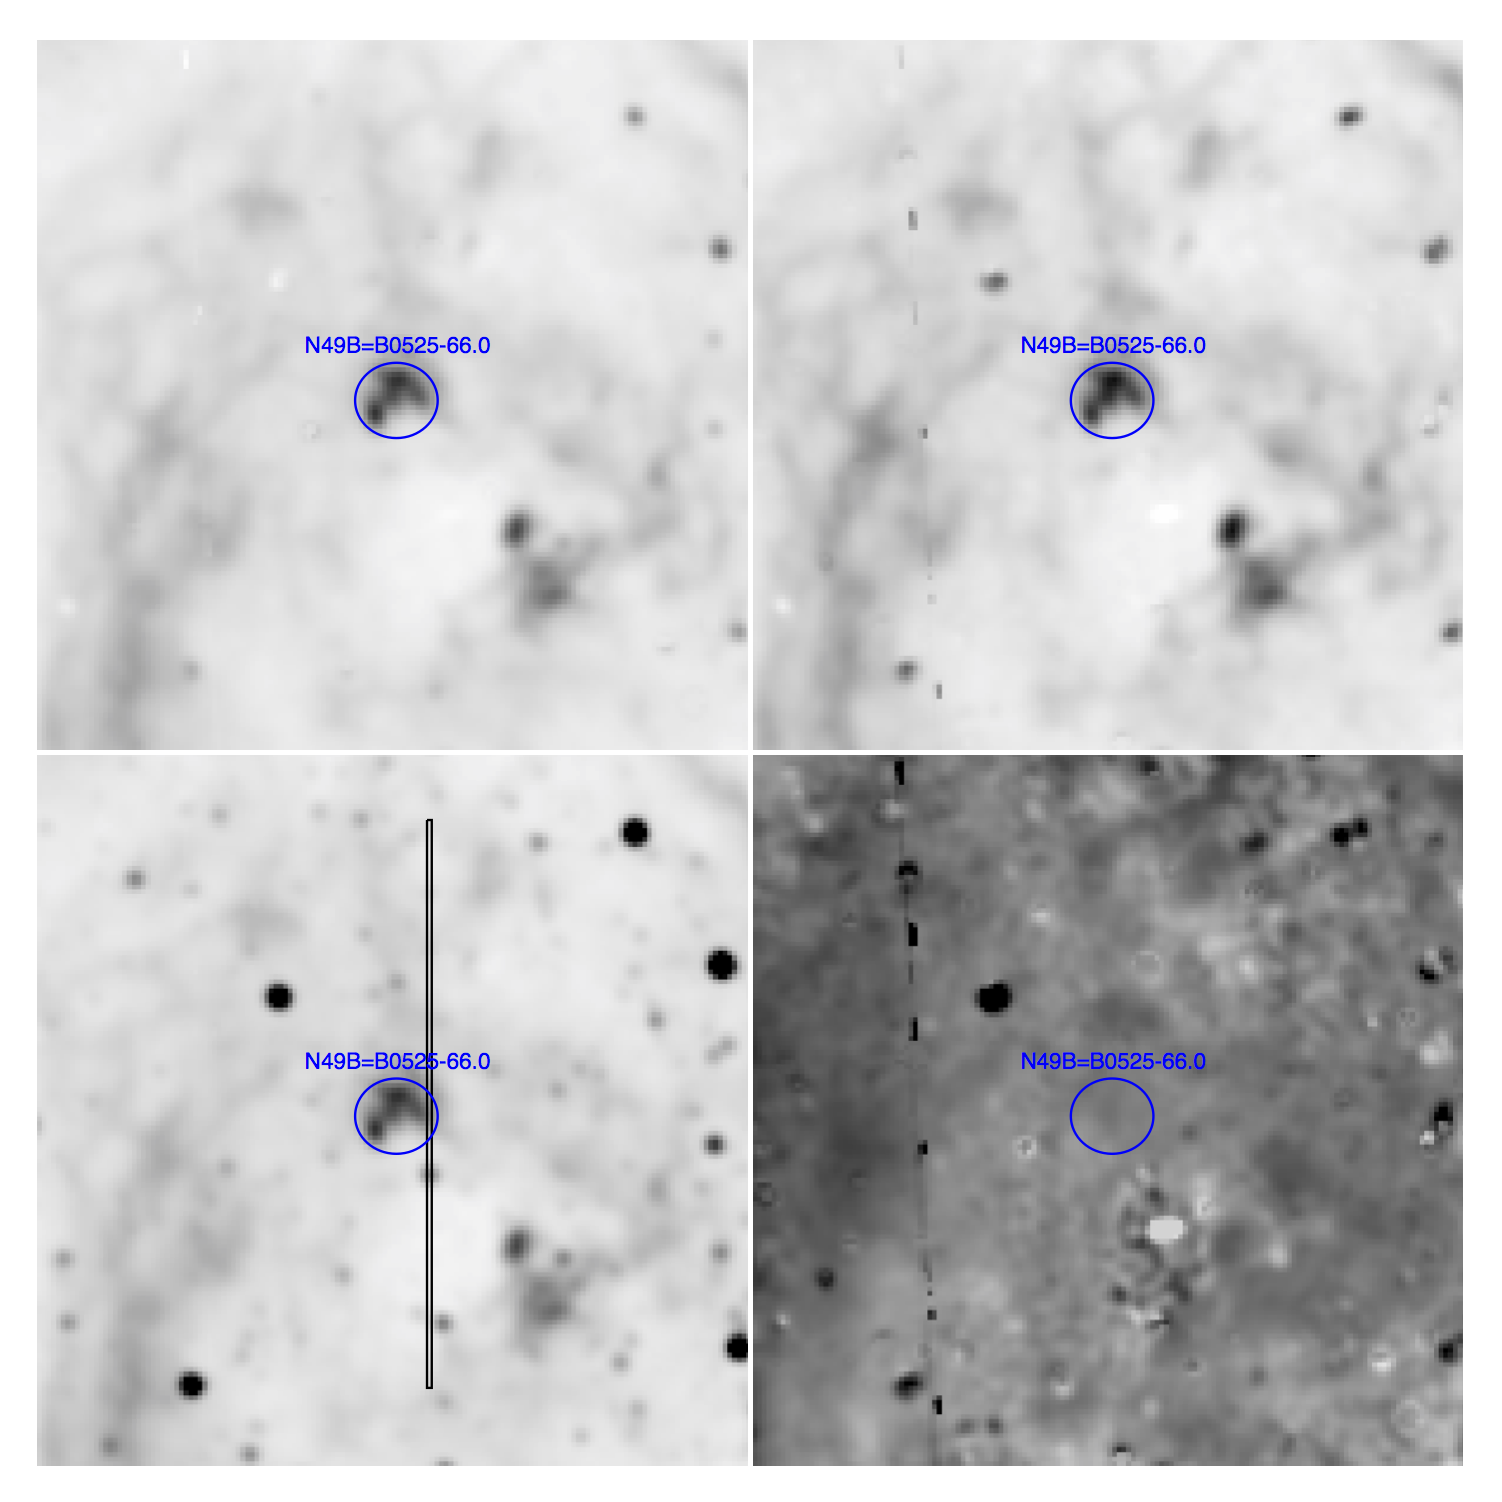
\includegraphics[width=10.05cm]{snapshots/N49B_5arcmin.png}
\end{figure}

\newpage
{\bf J0526-6604 = N49 = B0525-66.1 (5 arcmin field)}  
 
Slit Center:   5:25:54.783   -66:04:51.030 N-S

Scan:  East

Scan rate:  

Date/Frames:

Exposure Times:  

\begin{figure}
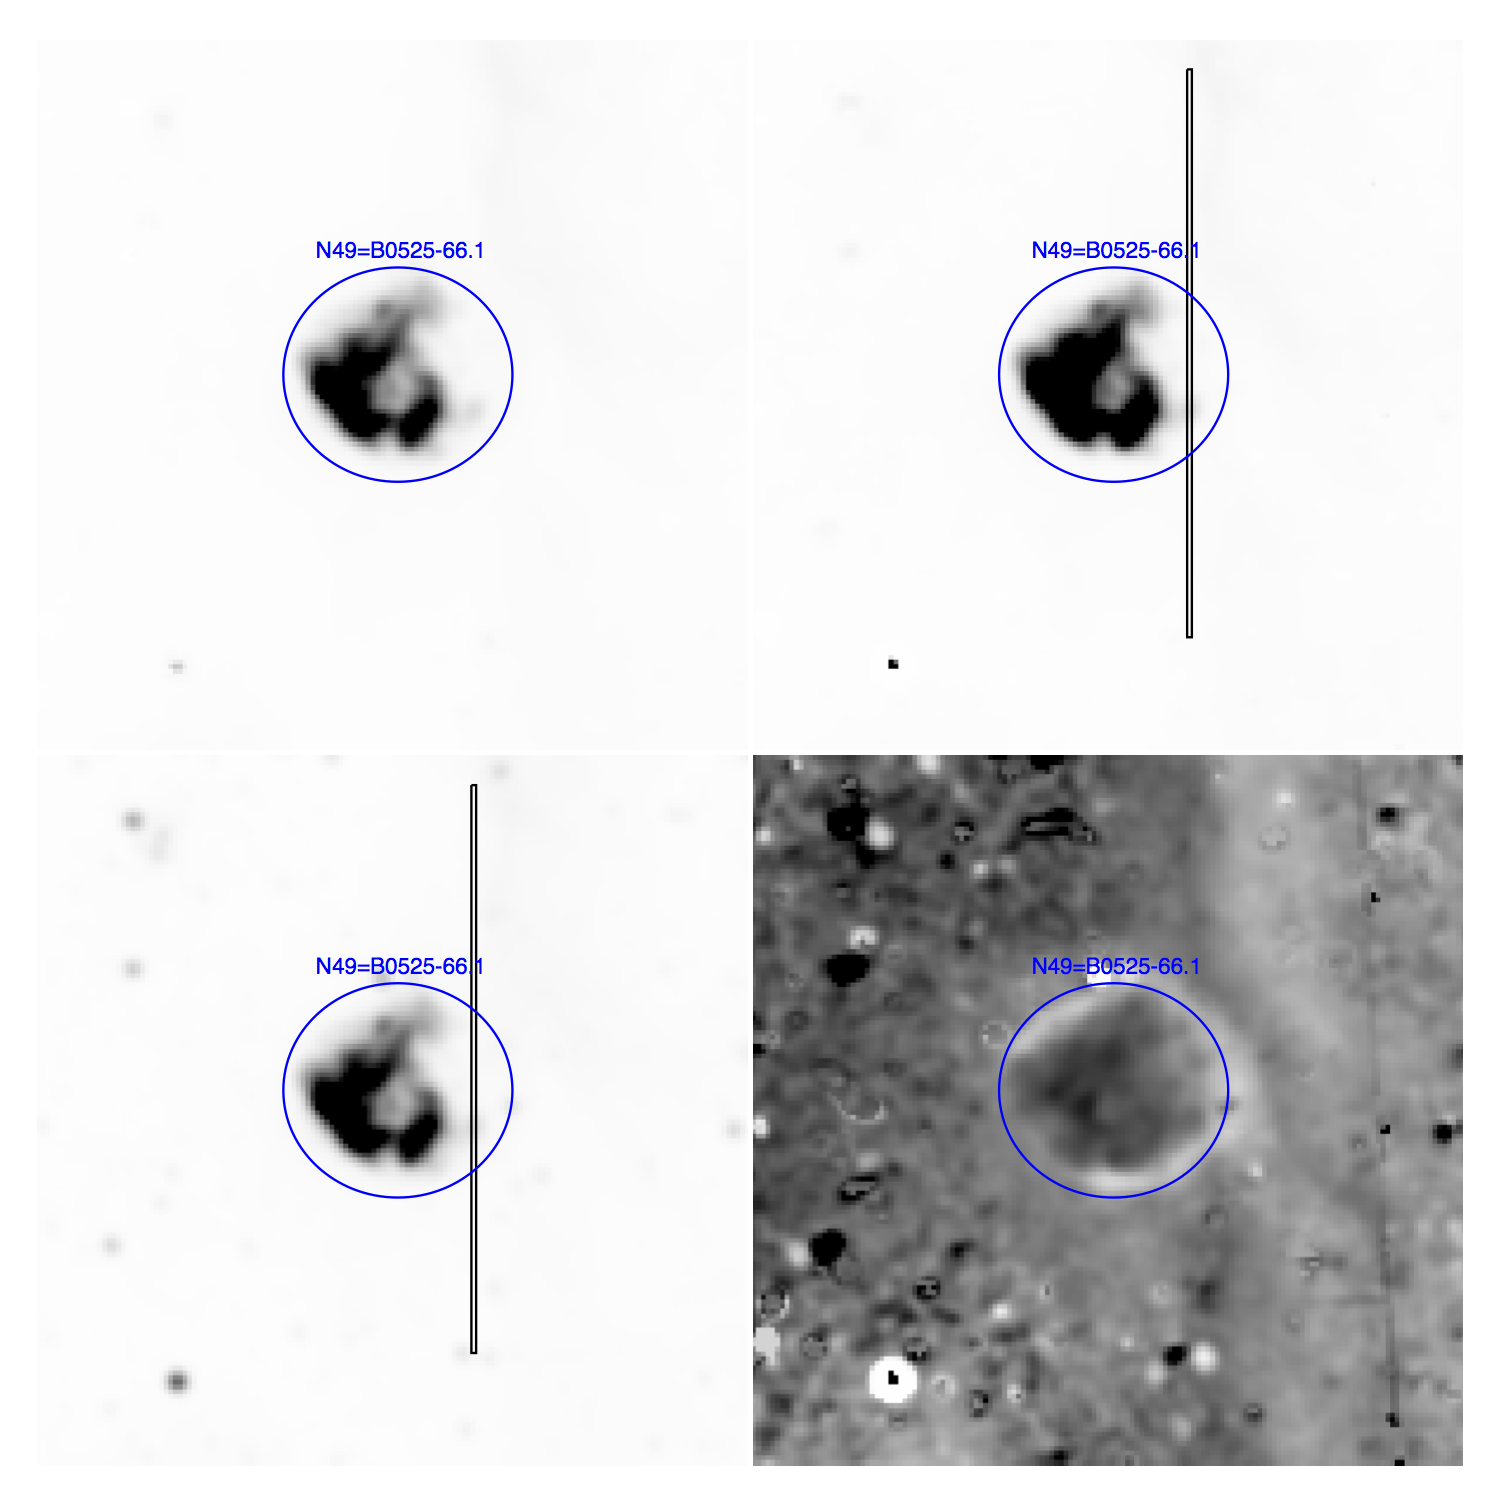
\includegraphics[width=10.05cm]{snapshots/N49_5arcmin.png}
\end{figure}

\newpage
{\bf J0527-6912 = B0528-67.2}  
 
Slit Center:   5:27:24.822  -69:12:07.609 N-S

Scan:  East

Scan rate:  

Date/Frames:

Exposure Times:  

\begin{figure}
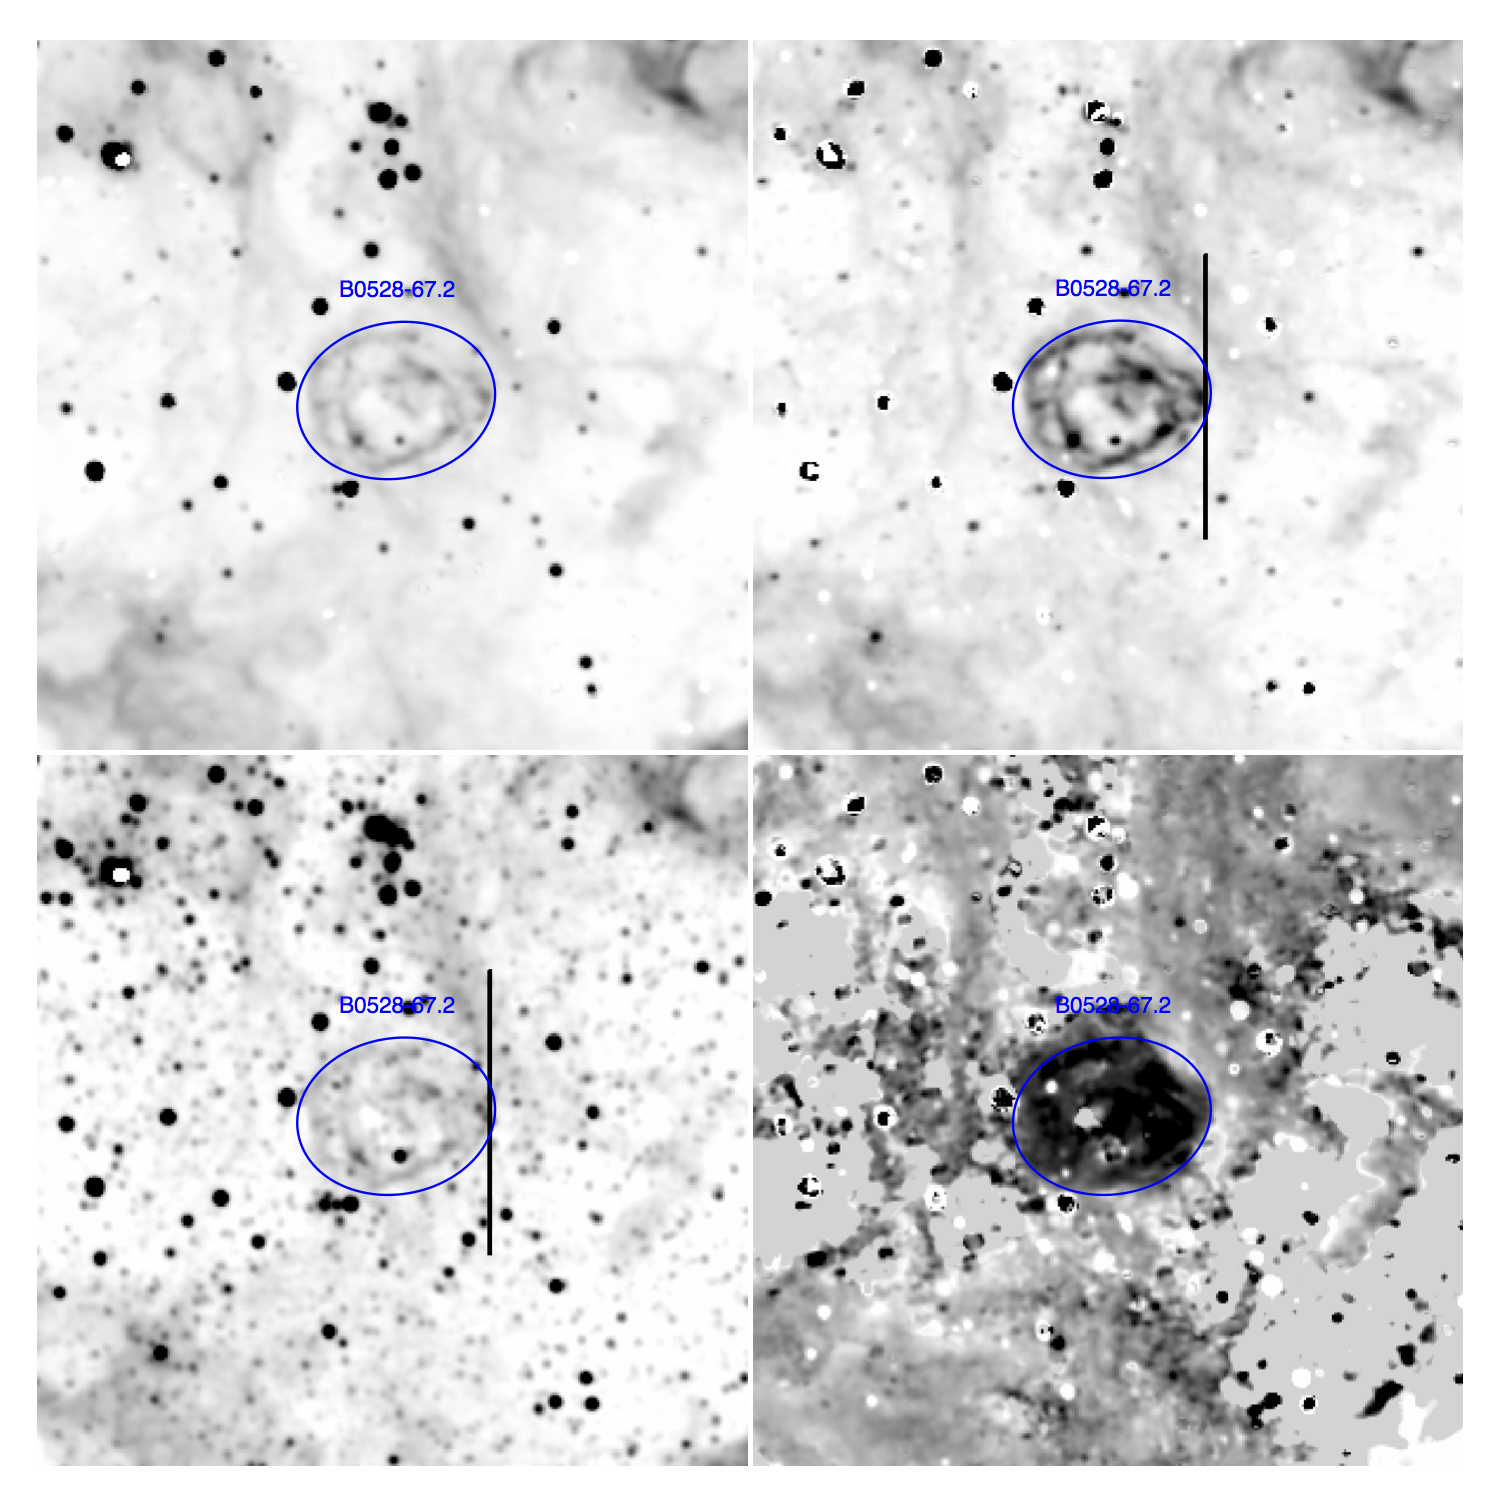
\includegraphics[width=10.05cm]{snapshots/B0528-672.png}
\end{figure}

\newpage
{\bf J0527-6549 = B0527-65.8 = DEML204}  
 
Slit Center:   none; this one is TOO BIG

Scan:  East

Scan rate:  

Date/Frames:

Exposure Times:  

No snapshot yet
\begin{figure}
%\includegraphics[width=10.05cm]{snapshots/xxx.png}
\end{figure}

\newpage
{\bf J0528-7104}  
 
Slit Center:   5:28:04.784,-71:07:11.216  E-W

Scan:  North

Scan rate:  

Date/Frames:

Exposure Times:  

\begin{figure}
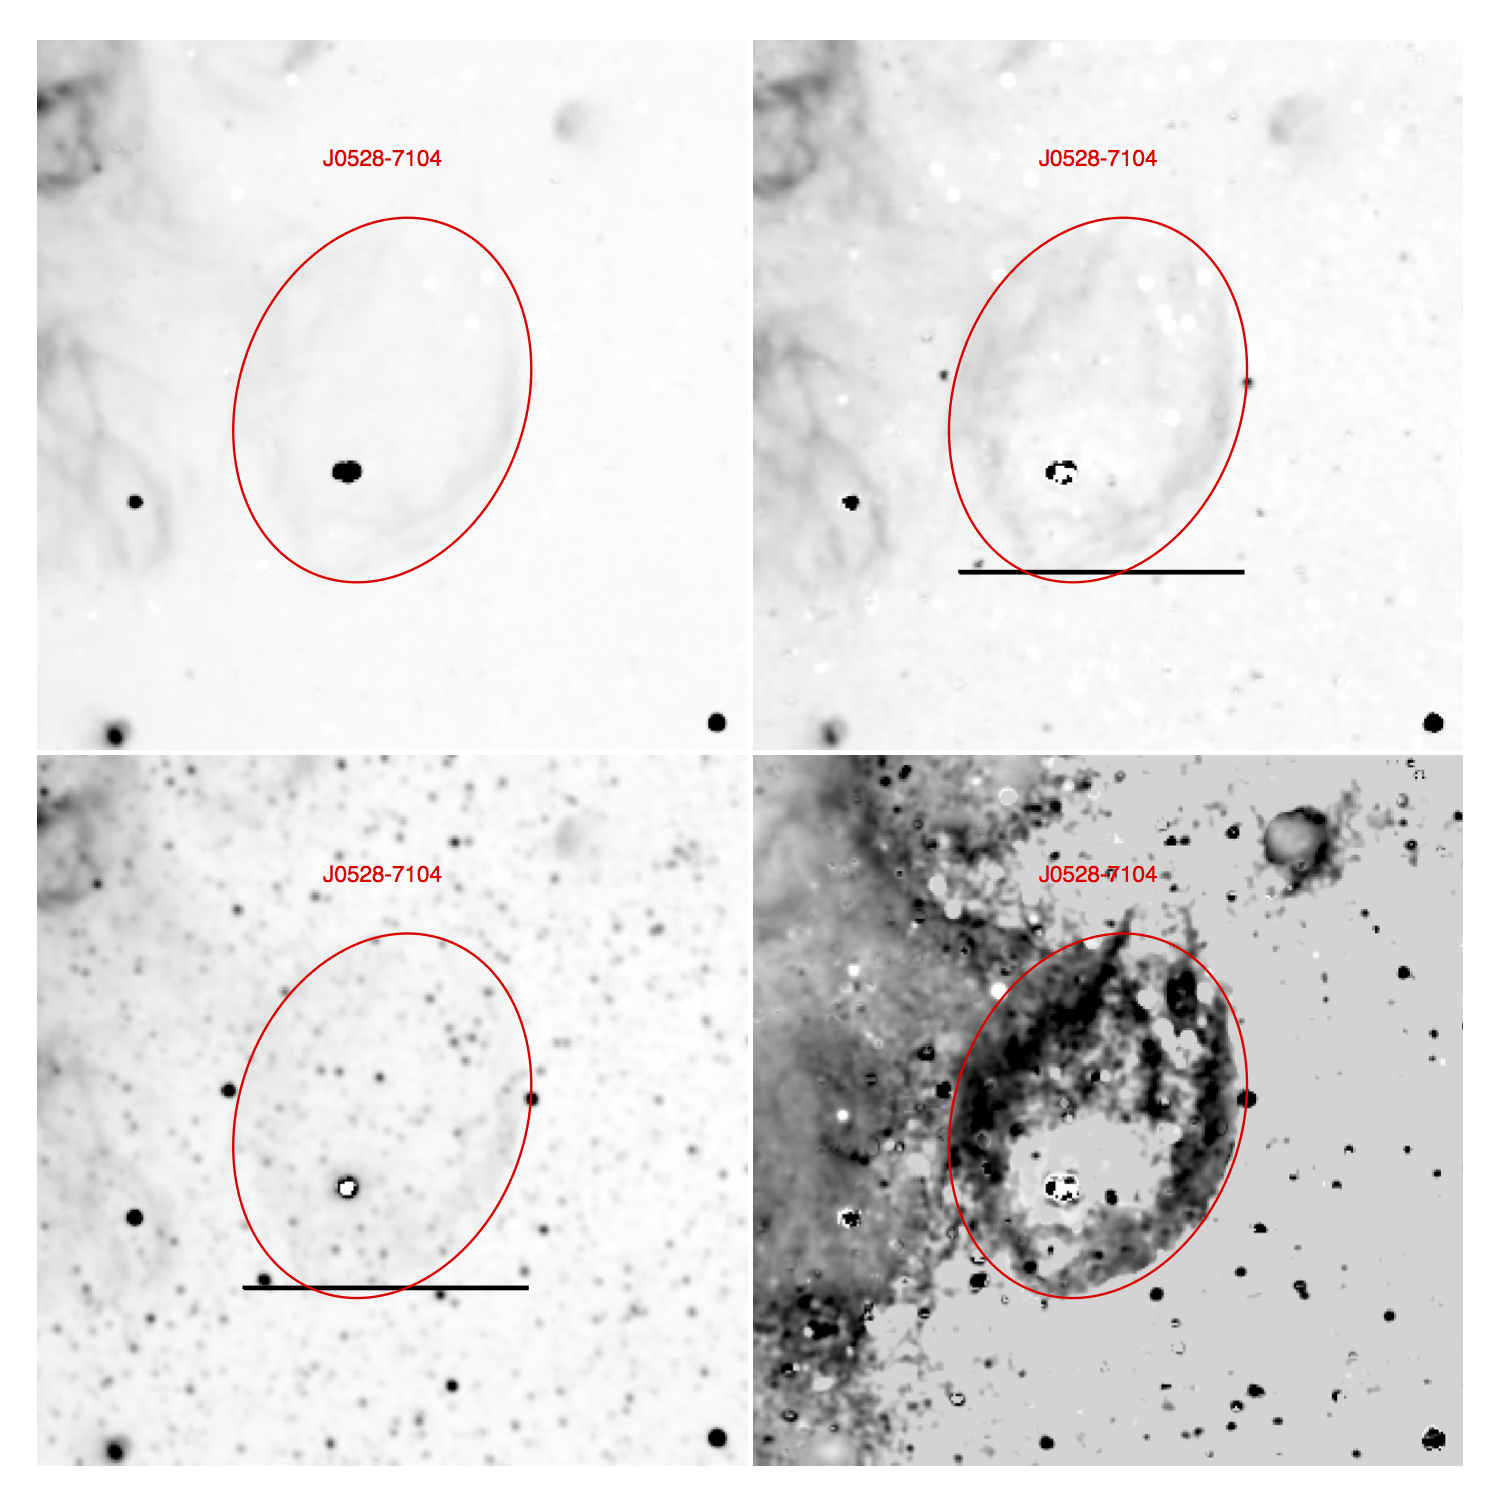
\includegraphics[width=10.05cm]{snapshots/J0528-7104_big.png}
\end{figure}

\newpage
{\bf J0528-6726 = DEML20}  
 
Slit Center:   5:28:12.992  -67:29:01.863  E-W

Scan:  North

Scan rate:  

Date/Frames:

Exposure Times:  

\begin{figure}
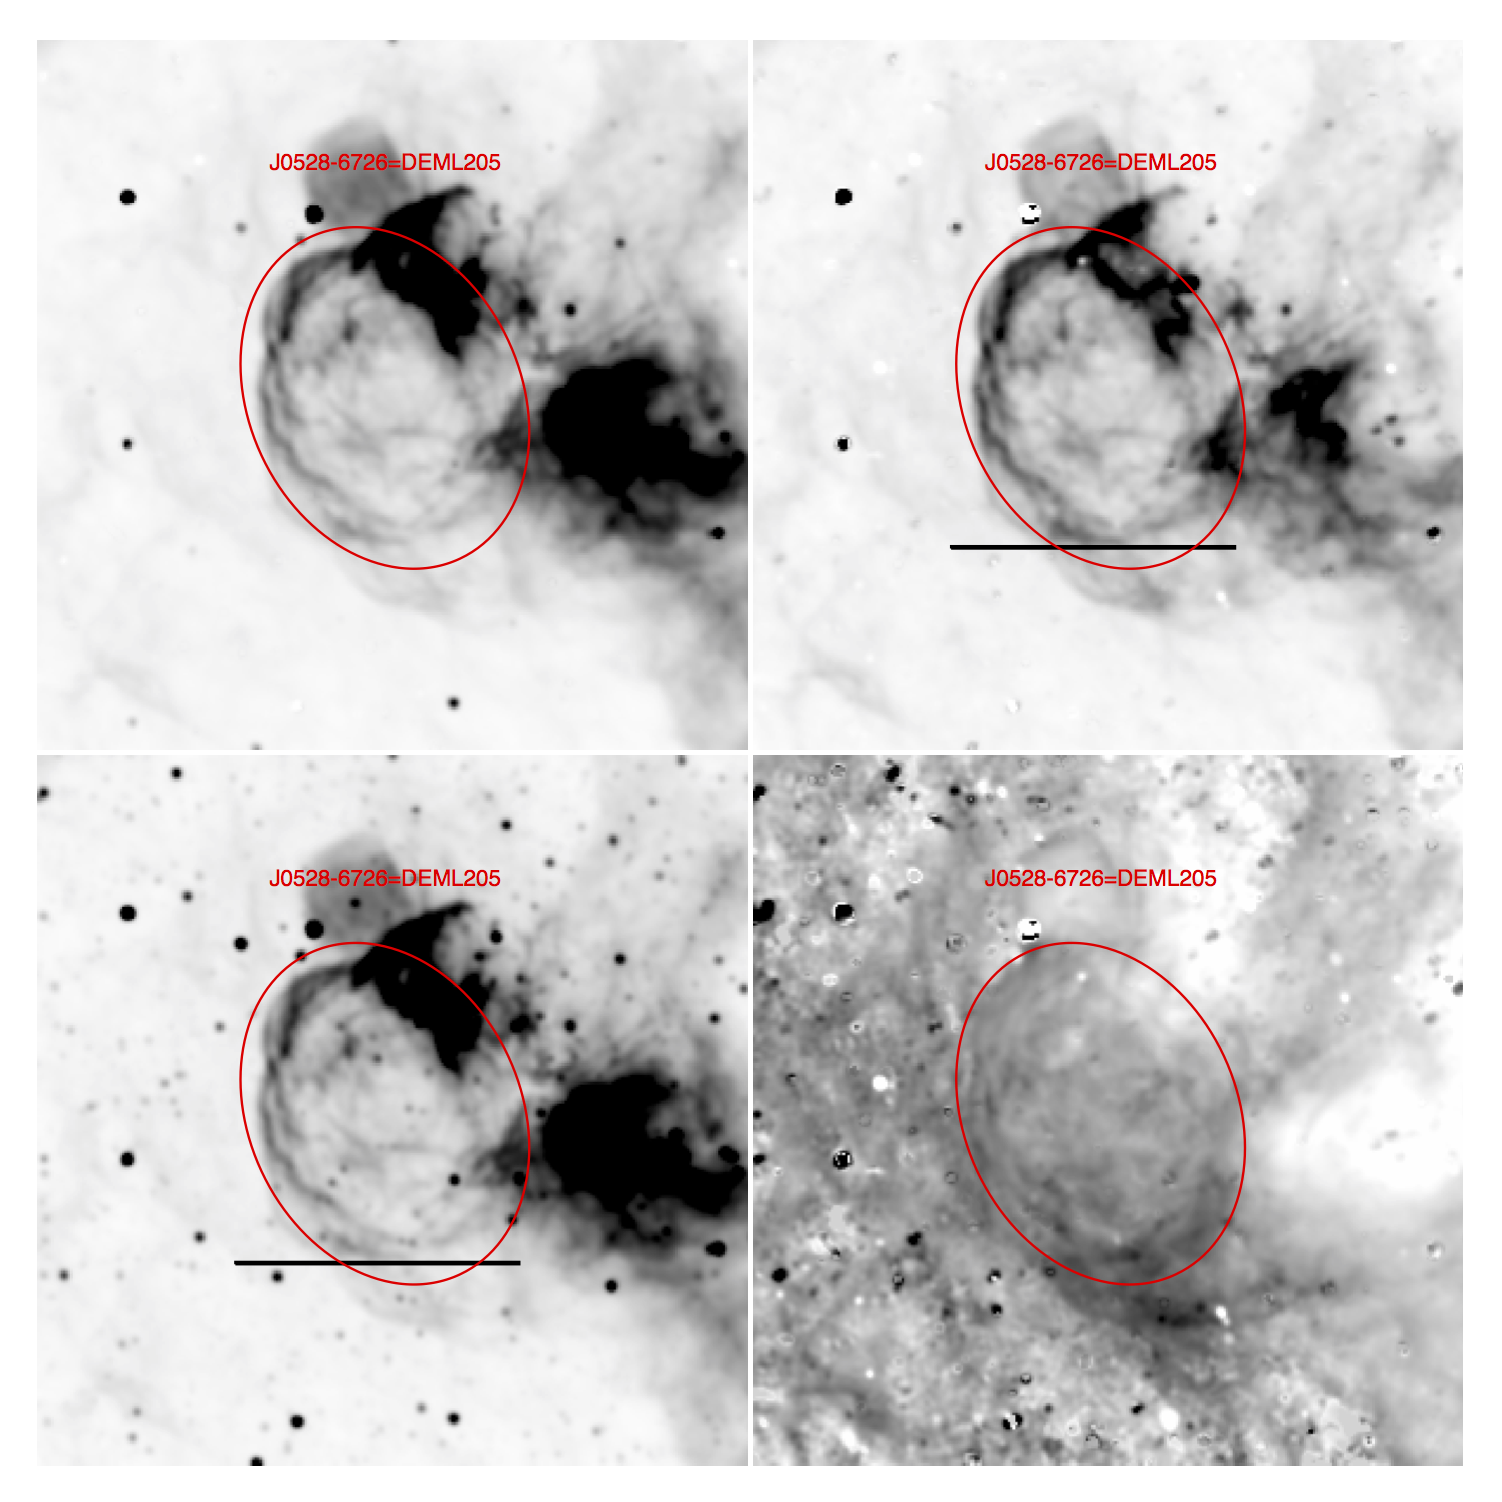
\includegraphics[width=10.05cm]{snapshots/J0528-6726.png}
\end{figure}

\newpage
{\bf J0530-7007 = DEML218}  
 
Slit Center:   5:30:16.284   -70:07:11.822 N-S

Scan:  East

Scan rate:  

Date/Frames:

Exposure Times:  

\begin{figure}
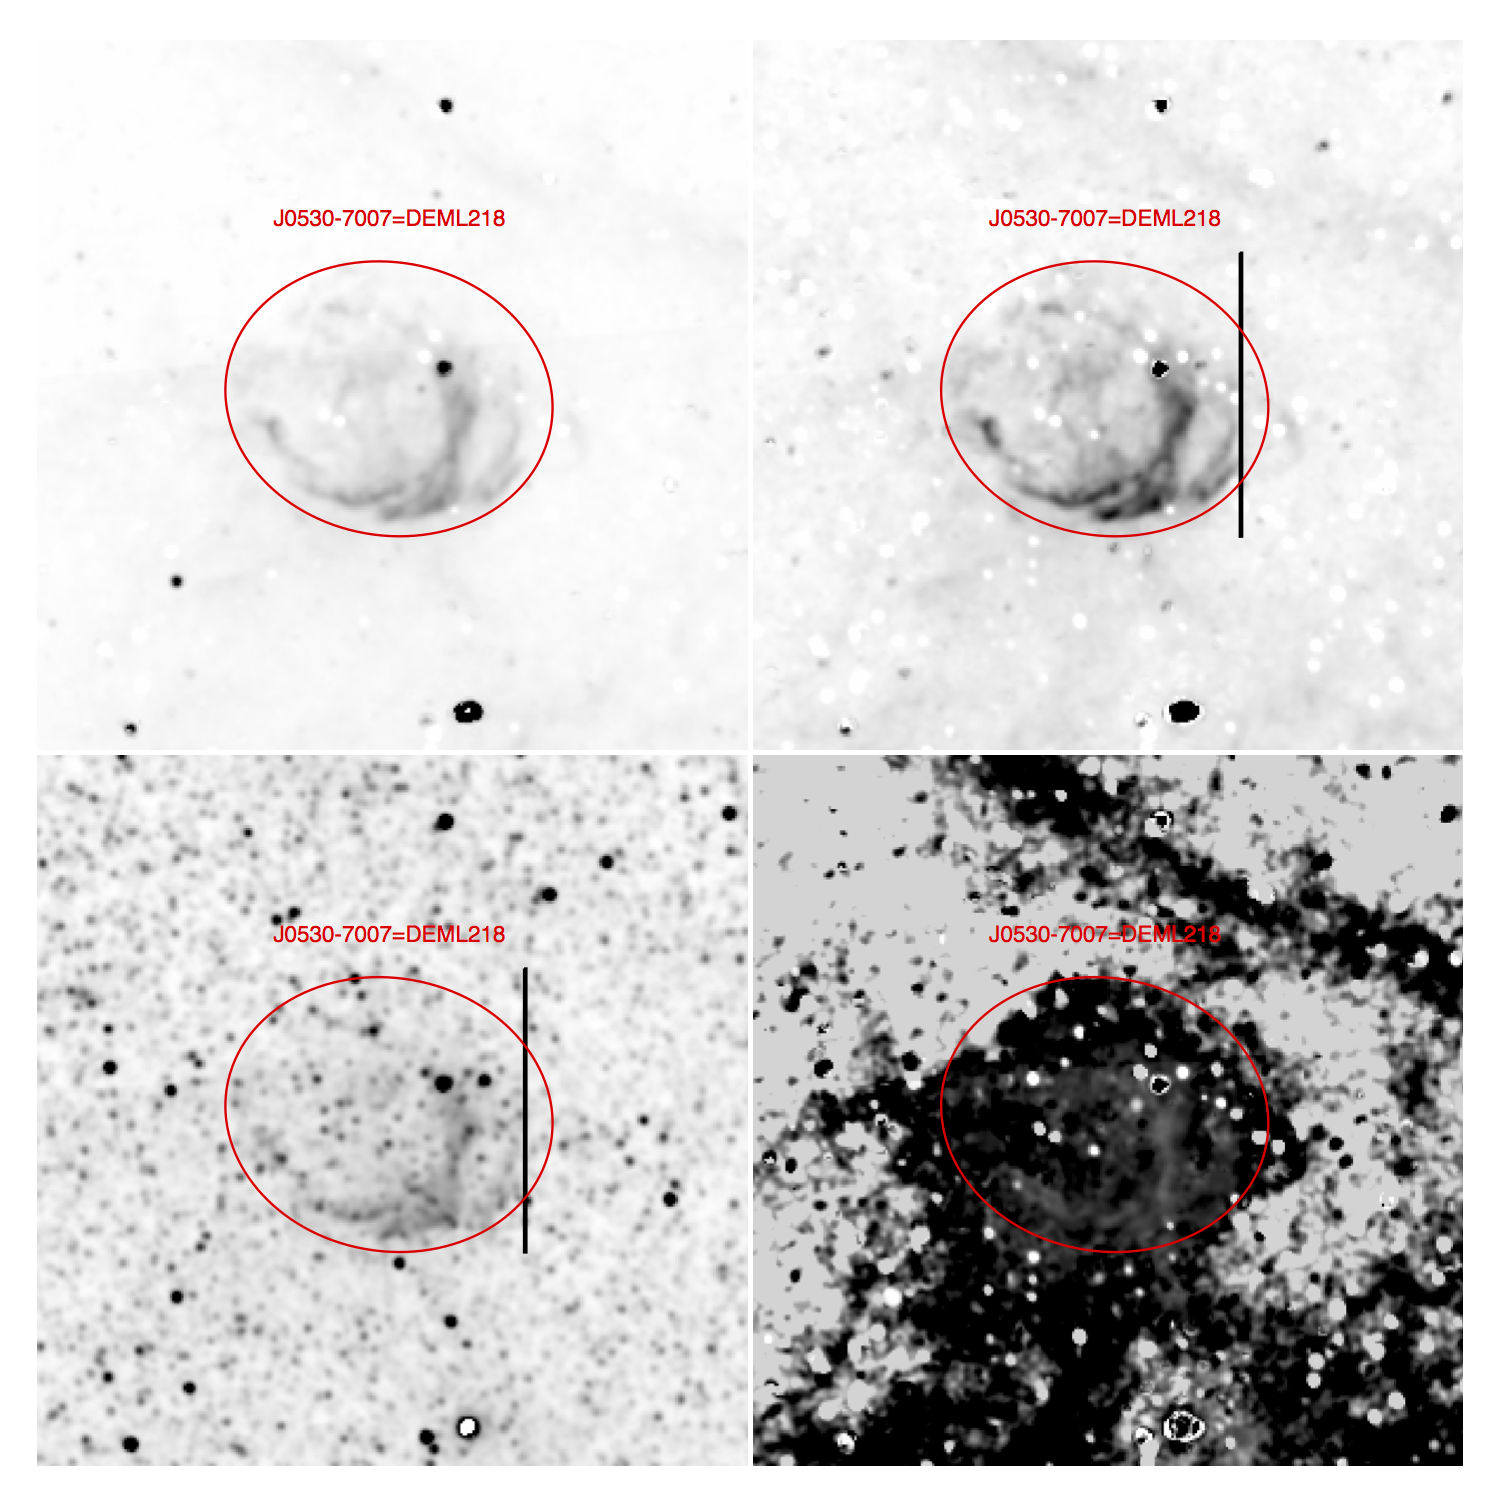
\includegraphics[width=10.05cm]{snapshots/J0530-7007.png}
\end{figure}

\newpage
{\bf J0531-7100 = B0532-71.0 = N206}  
 
Slit Center:   5:31:36.825   -71:00:05.057 N-S

Scan:  East

Scan rate:  

Date/Frames:

Exposure Times:  

\begin{figure}
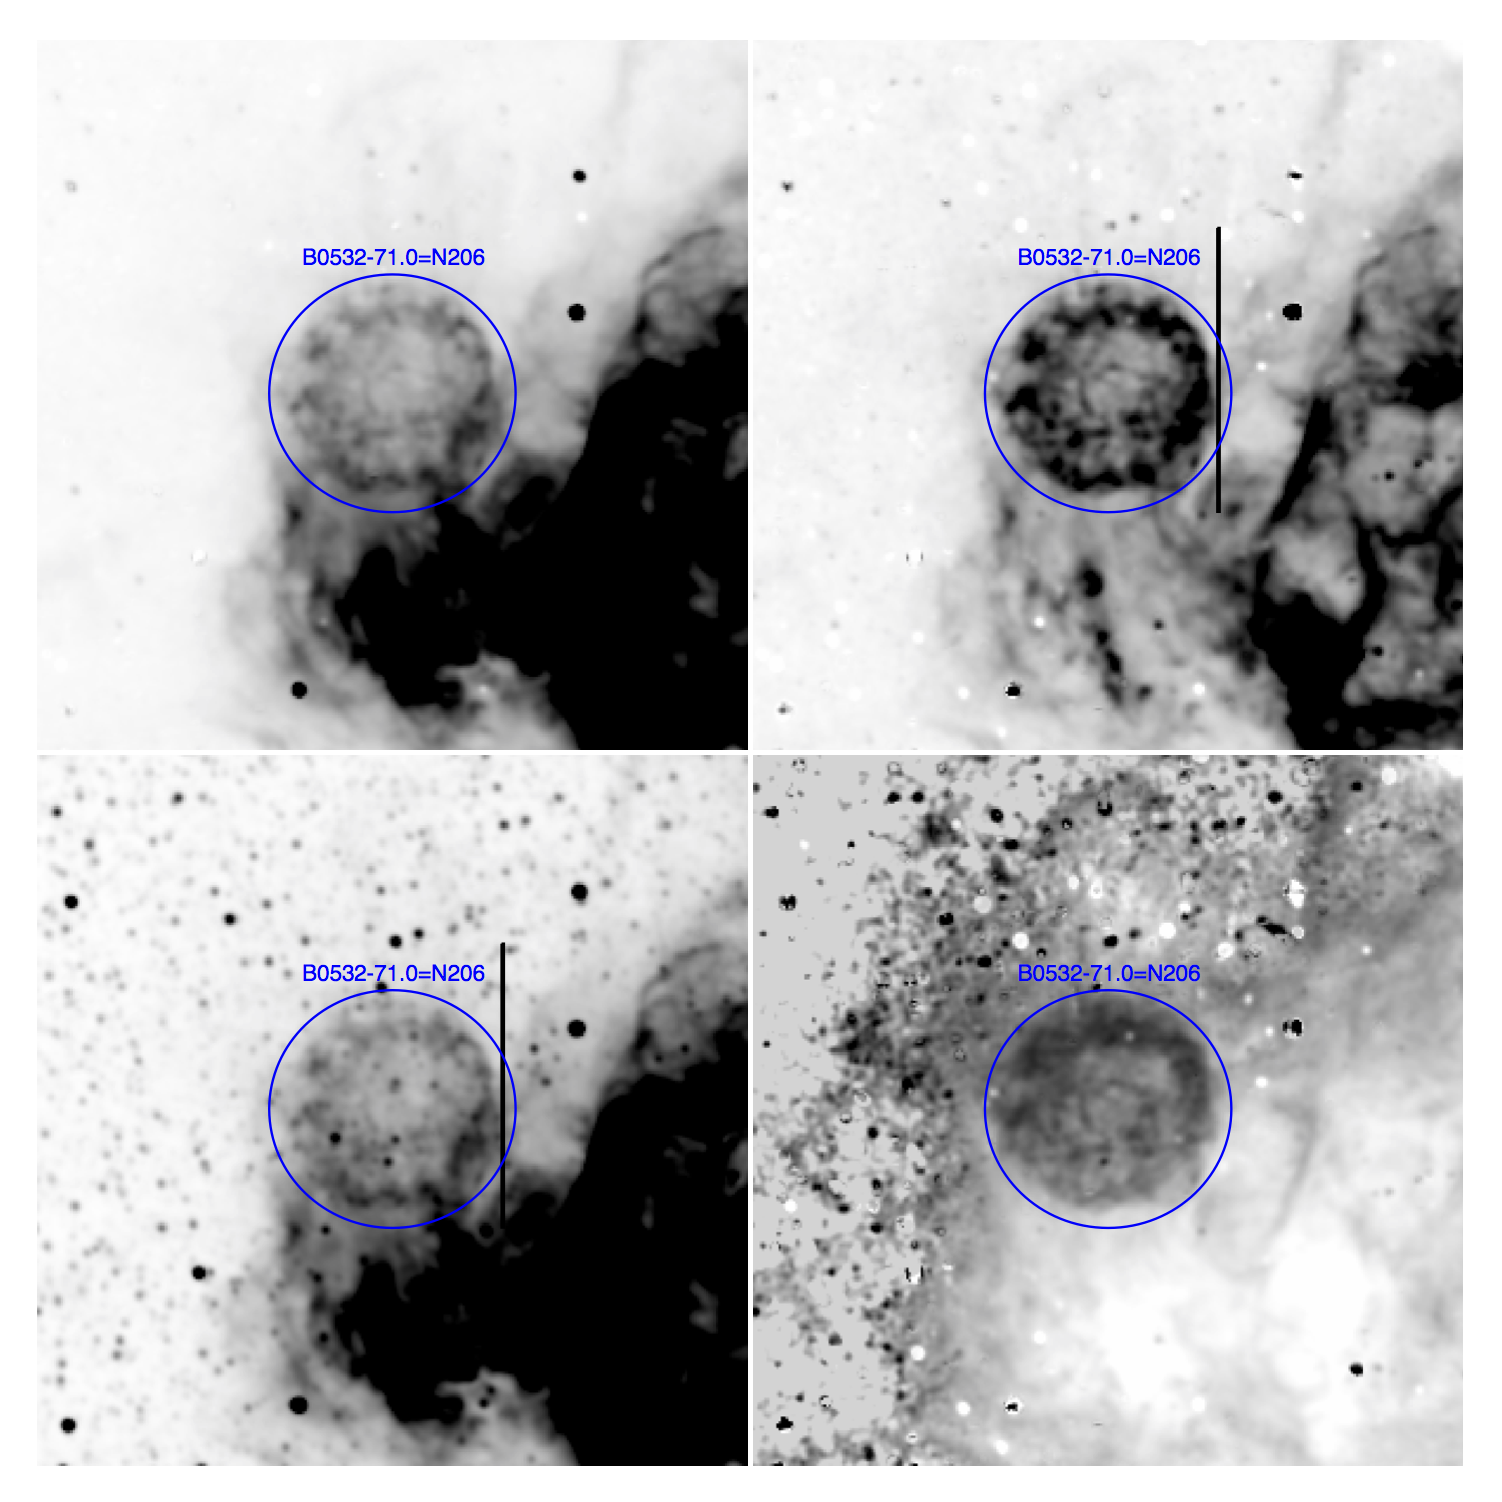
\includegraphics[width=10.05cm]{snapshots/B0532-710.png}
\end{figure}

\newpage
{\bf J0534-6955 = B0534-69.9}  
 
Slit Center:   5:33:51.783  -69:54:44.514  N-S

Scan:  East

Scan rate:  

Date/Frames:

Exposure Times:  

\begin{figure}
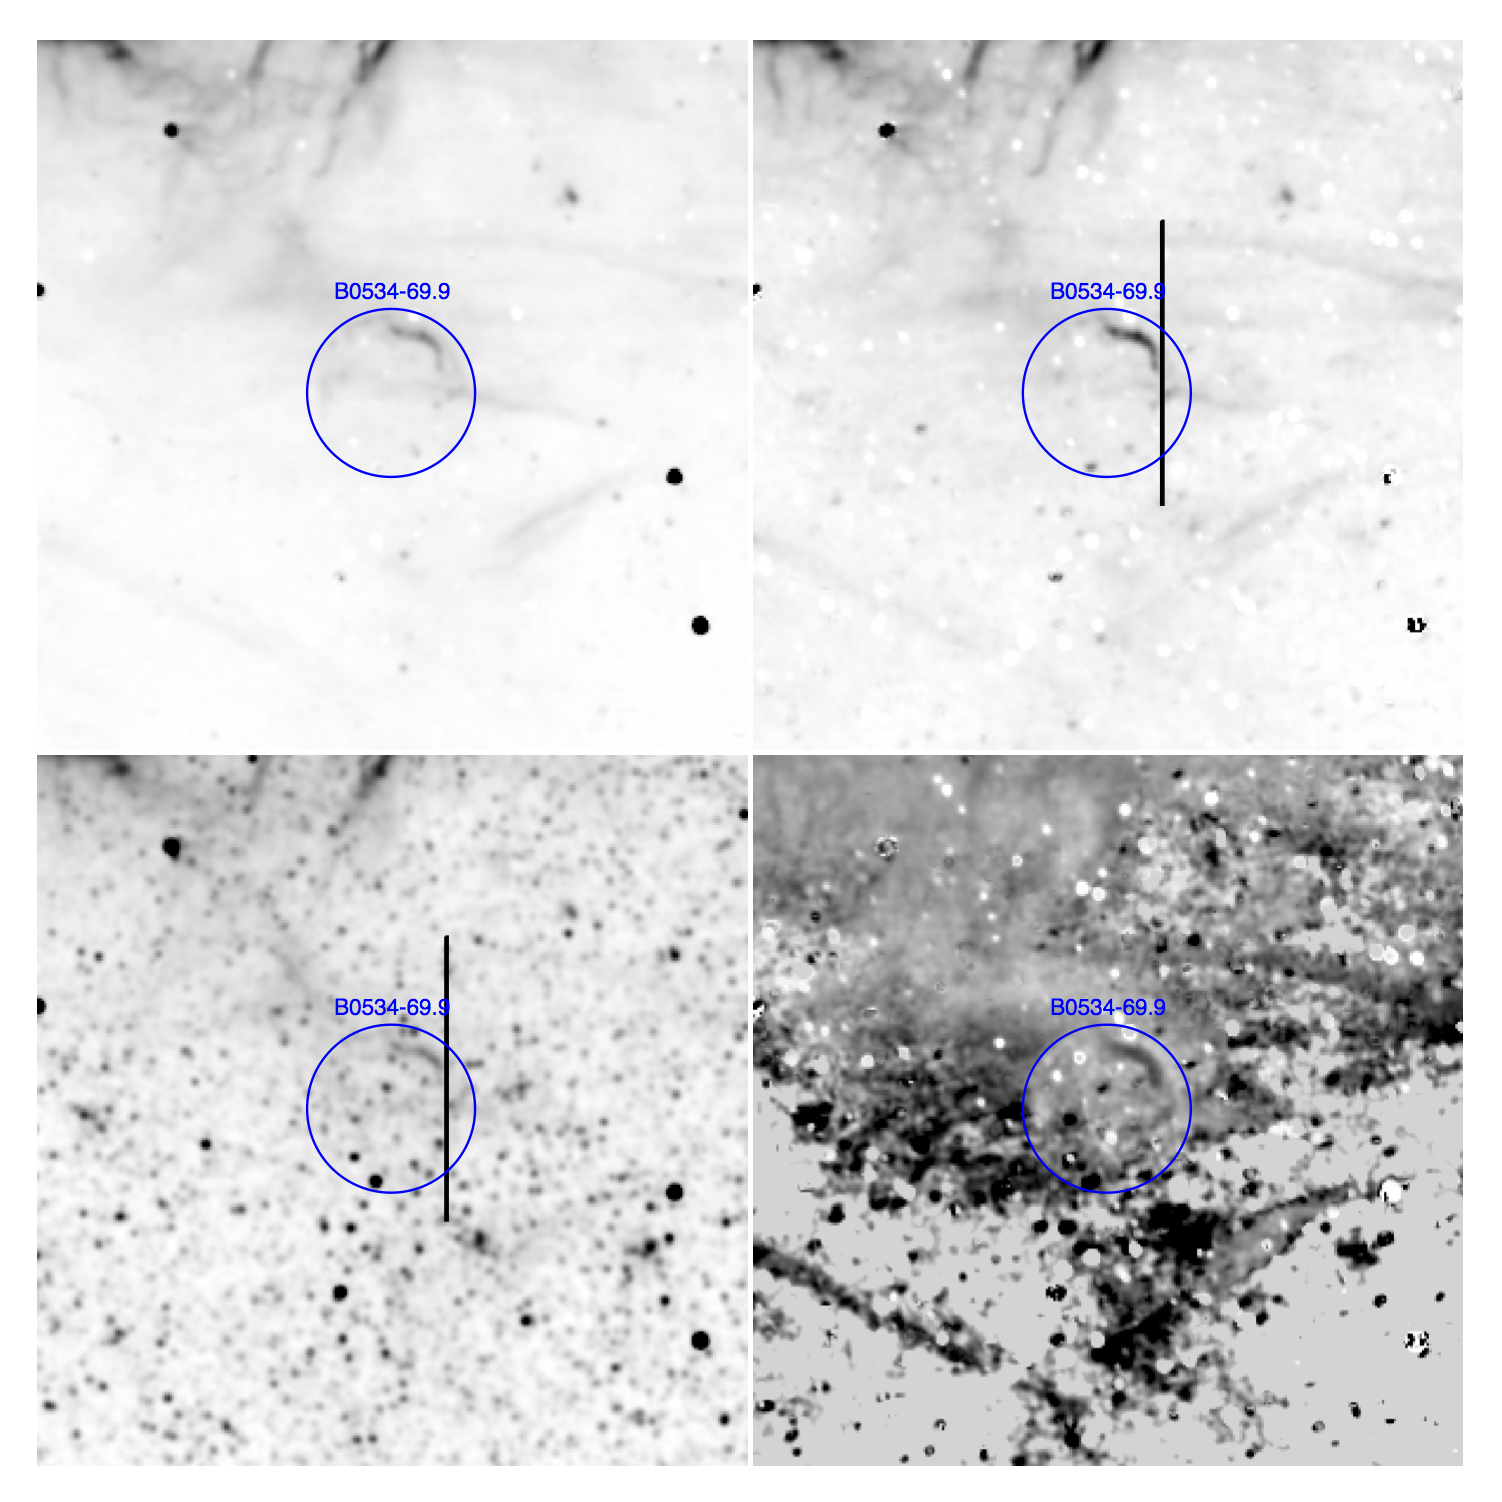
\includegraphics[width=10.05cm]{snapshots/B0534-699.png}
\end{figure}

\newpage
{\bf J0534-7033 = B0534-70.5 = DEML238}  
 
Slit Center:   5:34:01.781 -70:33:14.761  N-S

Scan:  East

Scan rate:  

Date/Frames:

Exposure Times:  

\begin{figure}
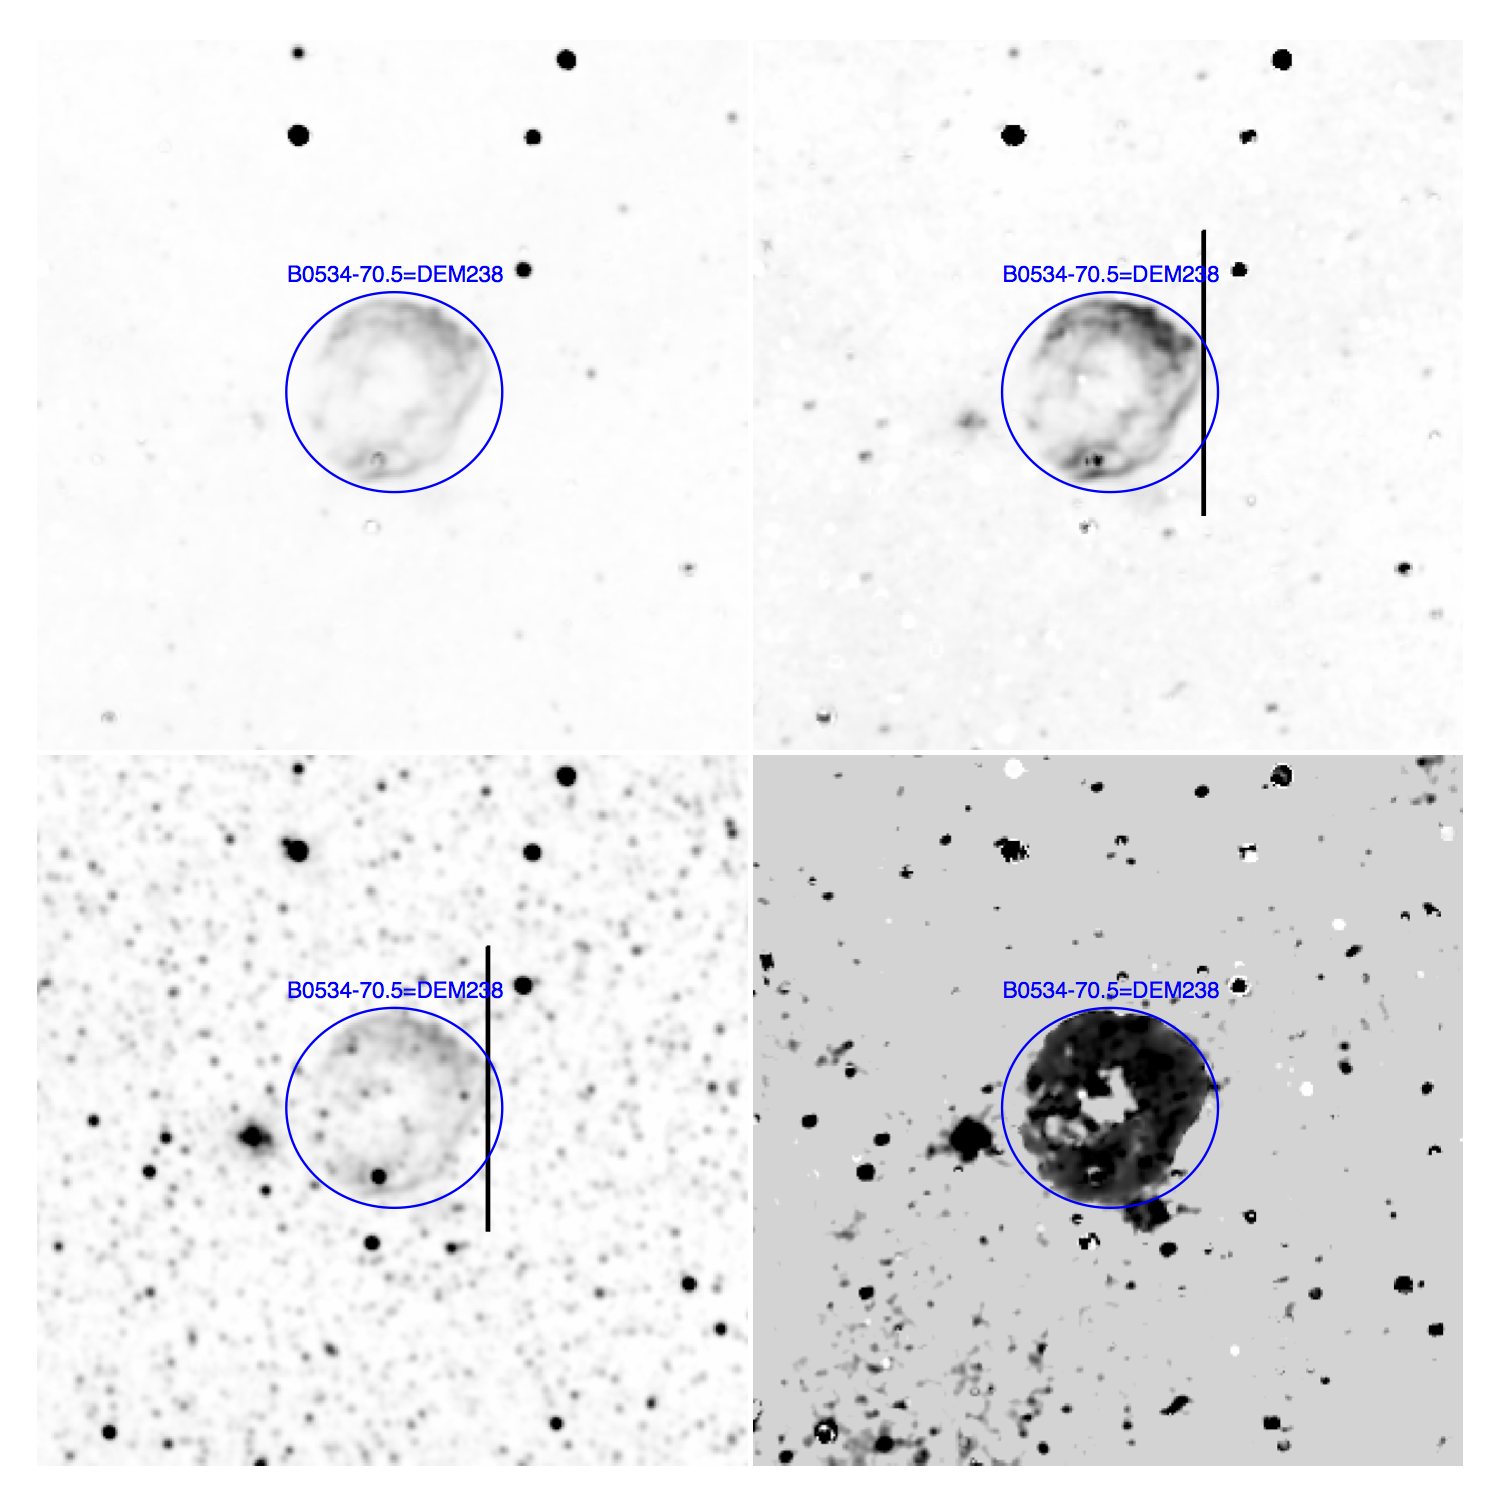
\includegraphics[width=10.05cm]{snapshots/B0534-705.png}
\end{figure}

\newpage
{\bf J0535-6602 = N63A = B0535-66.0   (5  arcmin field)}  
 
Slit Center:   5:35:40.412   -66:02:05.183   N-S

Scan:  East

Scan rate:  

Date/Frames:

Exposure Times:  

\begin{figure}
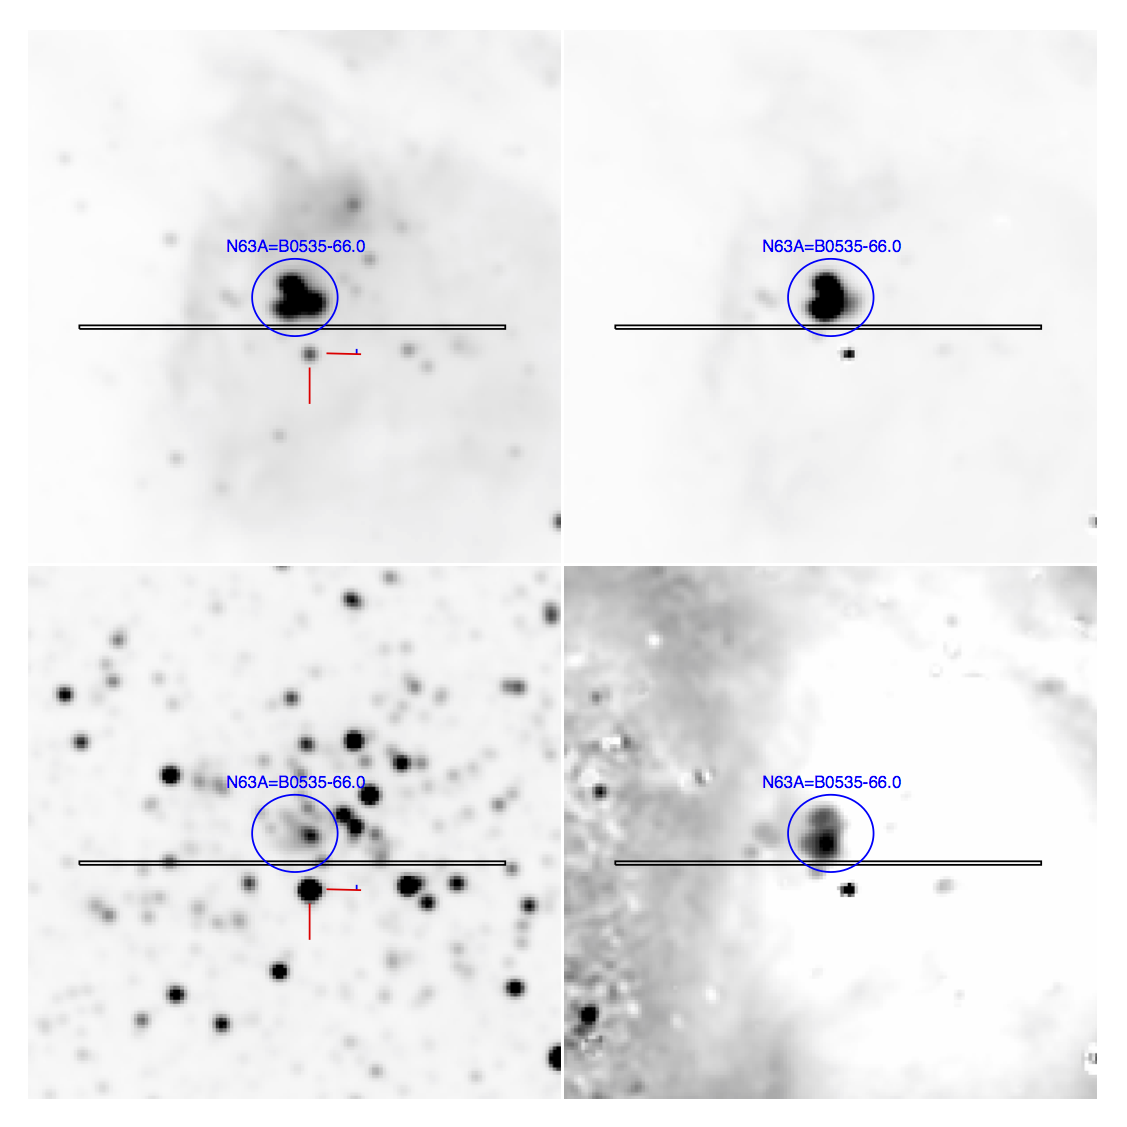
\includegraphics[width=10.05cm]{snapshots/N63A_5arcmin.png}
\end{figure}

\newpage
{\bf J0536-6735 = B0536-67.6}  
 
Slit Center:   5:36:04.295  -67:34:57.684  E-W

Scan:  South

Scan rate:  

Date/Frames:

Exposure Times:  

\begin{figure}
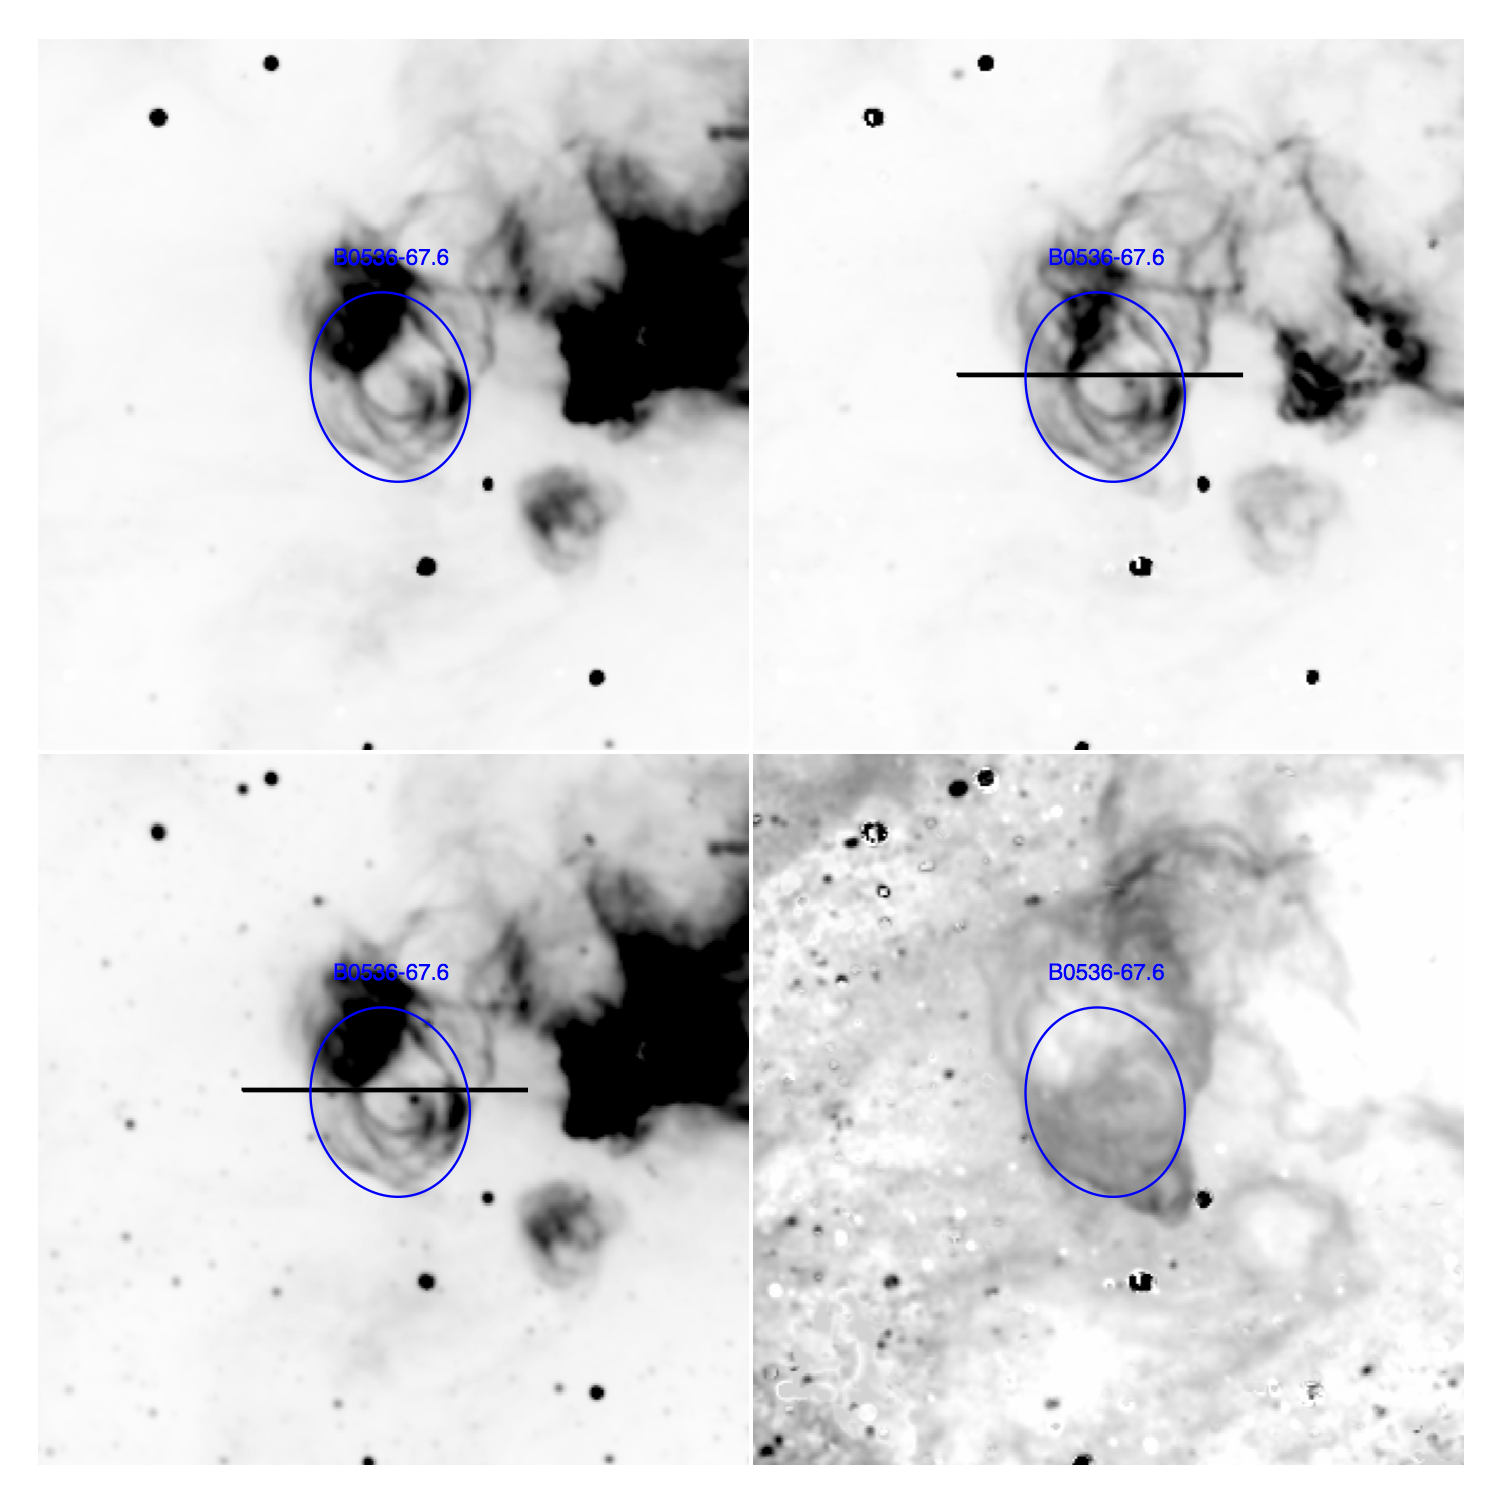
\includegraphics[width=10.05cm]{snapshots/B0536-676.png}
\end{figure}


\newpage
{\bf J0536-7038 = B0536-70.6 = DEM249}  
 
Slit Center:   5:35:50.282   -70:38:35.277 N-S

Scan:  East

Scan rate:  

Date/Frames:

Exposure Times:  

\begin{figure}
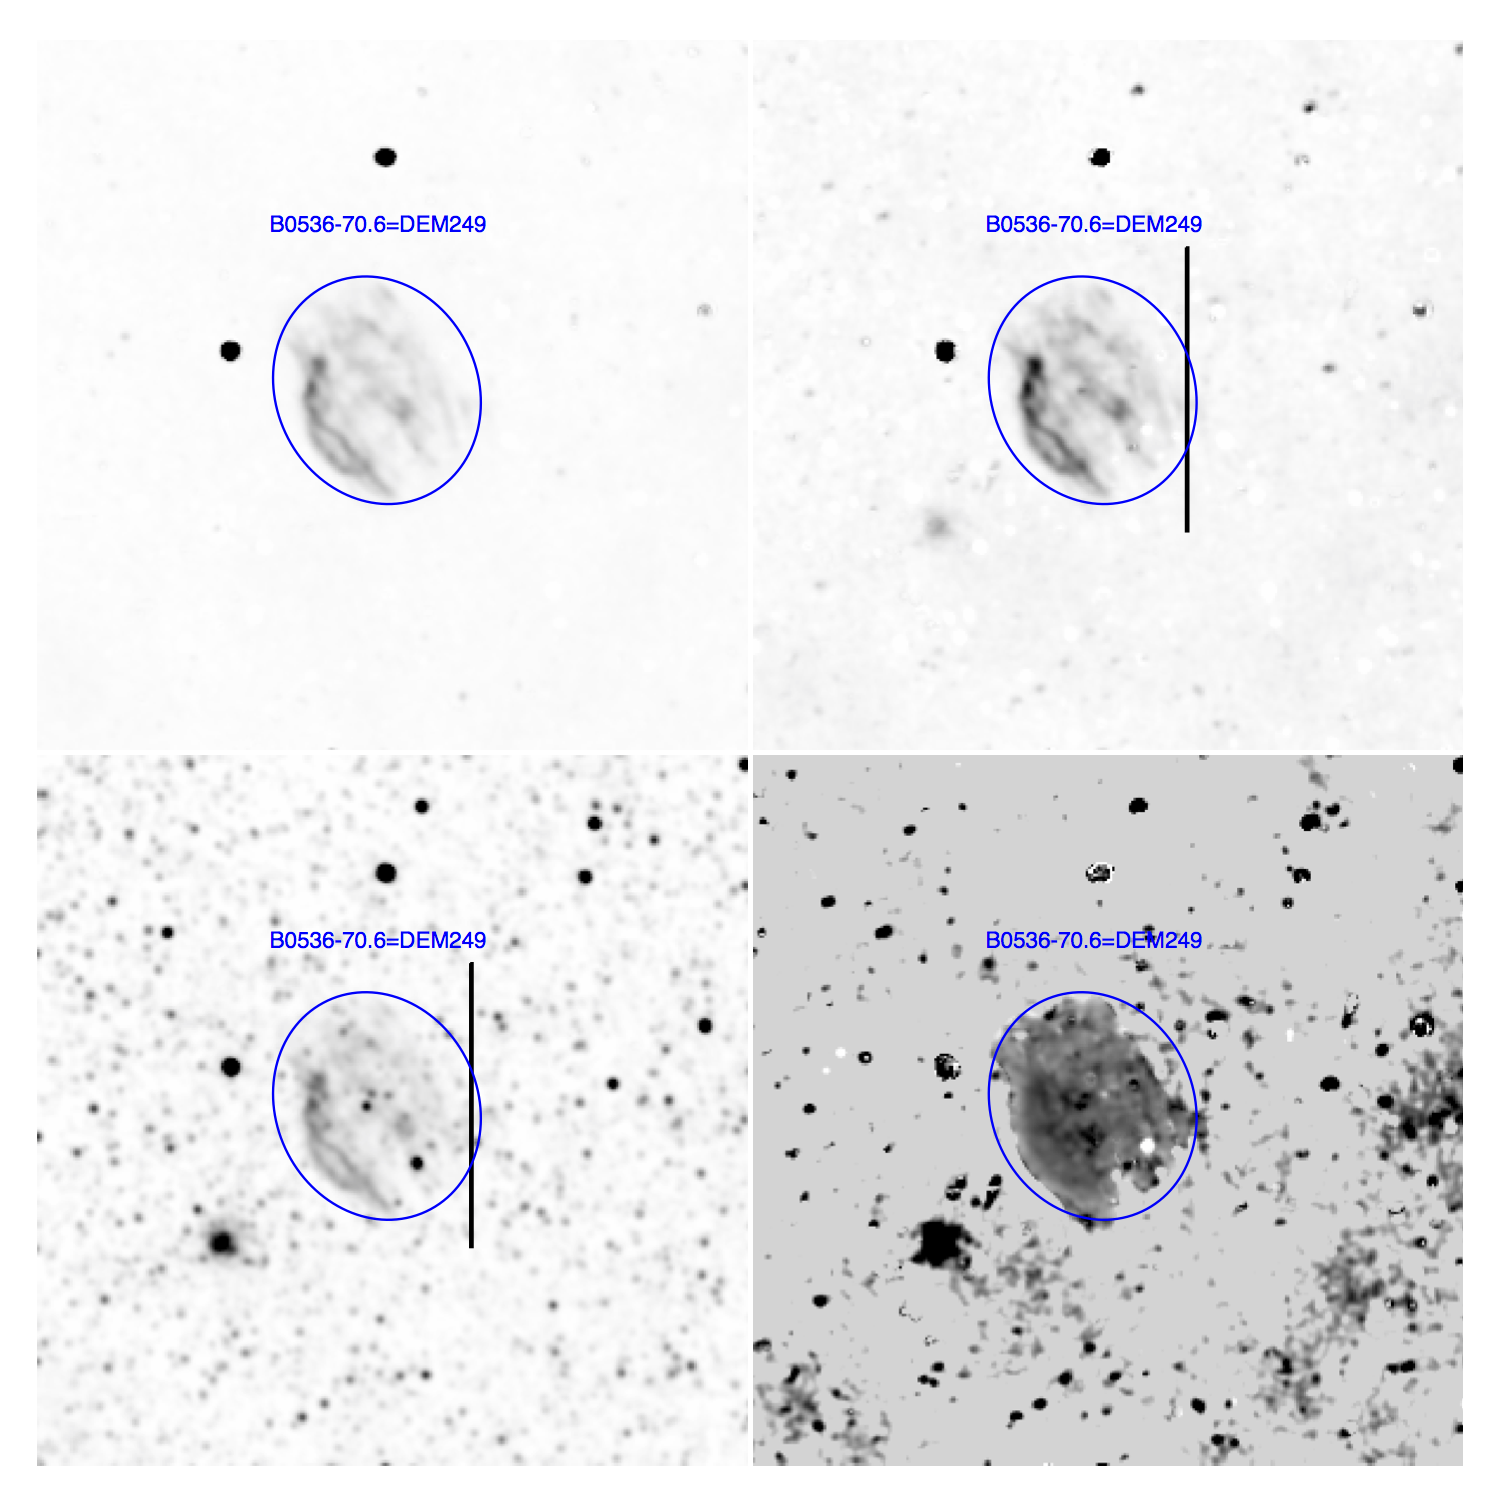
\includegraphics[width=10.05cm]{snapshots/B0536-706.png}
\end{figure}


\newpage
{\bf J0537-6639 (new)}  
 
Slit Center:   too big to scan

Scan:  East

Scan rate:  

Date/Frames:

Exposure Times:  

no snapshot
\begin{figure}
%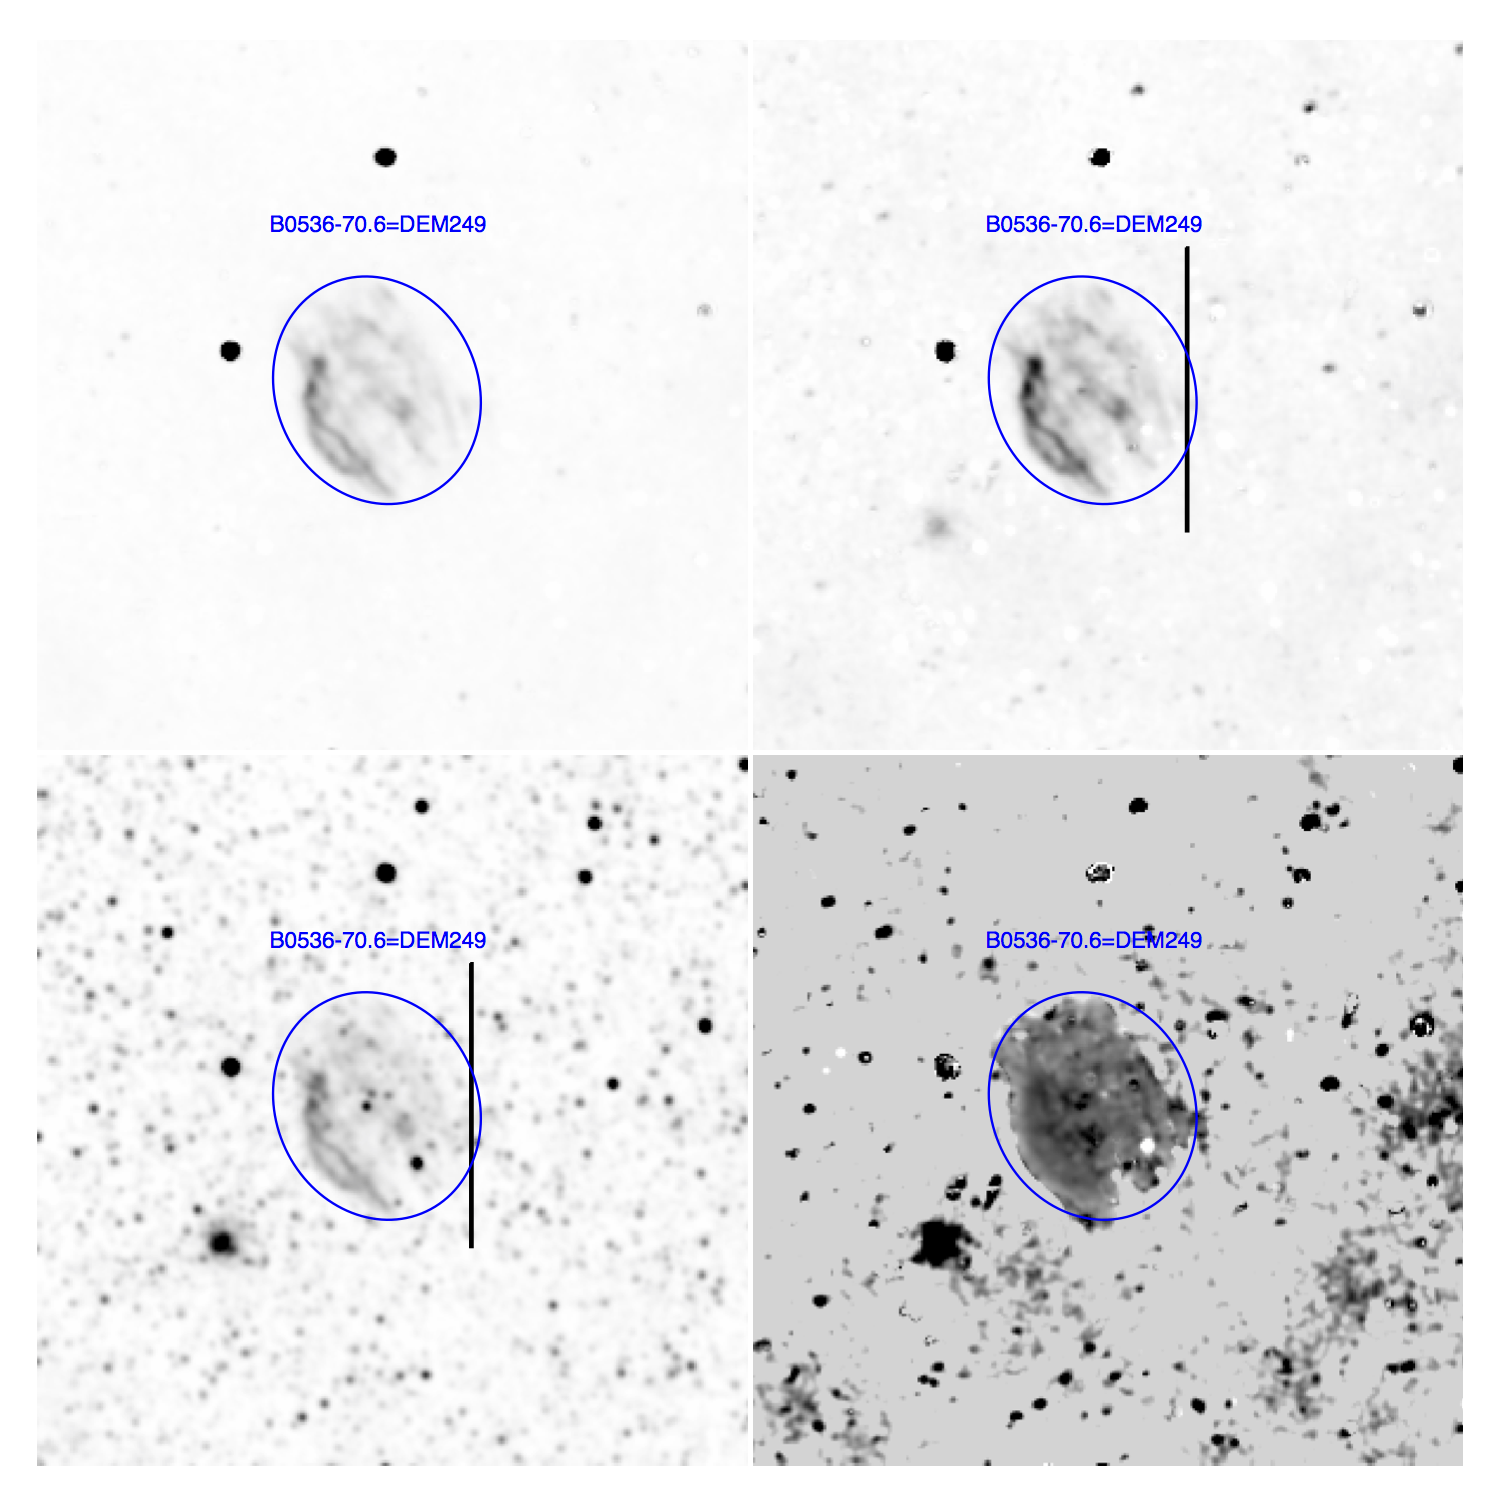
\includegraphics[width=10.05cm]{snapshots/B0536-706.png}
\end{figure}

\newpage
{\bf J0537-6627 = DEML256}  
 
Slit Center:  5:37:12.322  -66:27:51.629 N-S

Scan:  East

Scan rate:  

Date/Frames:

Exposure Times:  

\begin{figure}
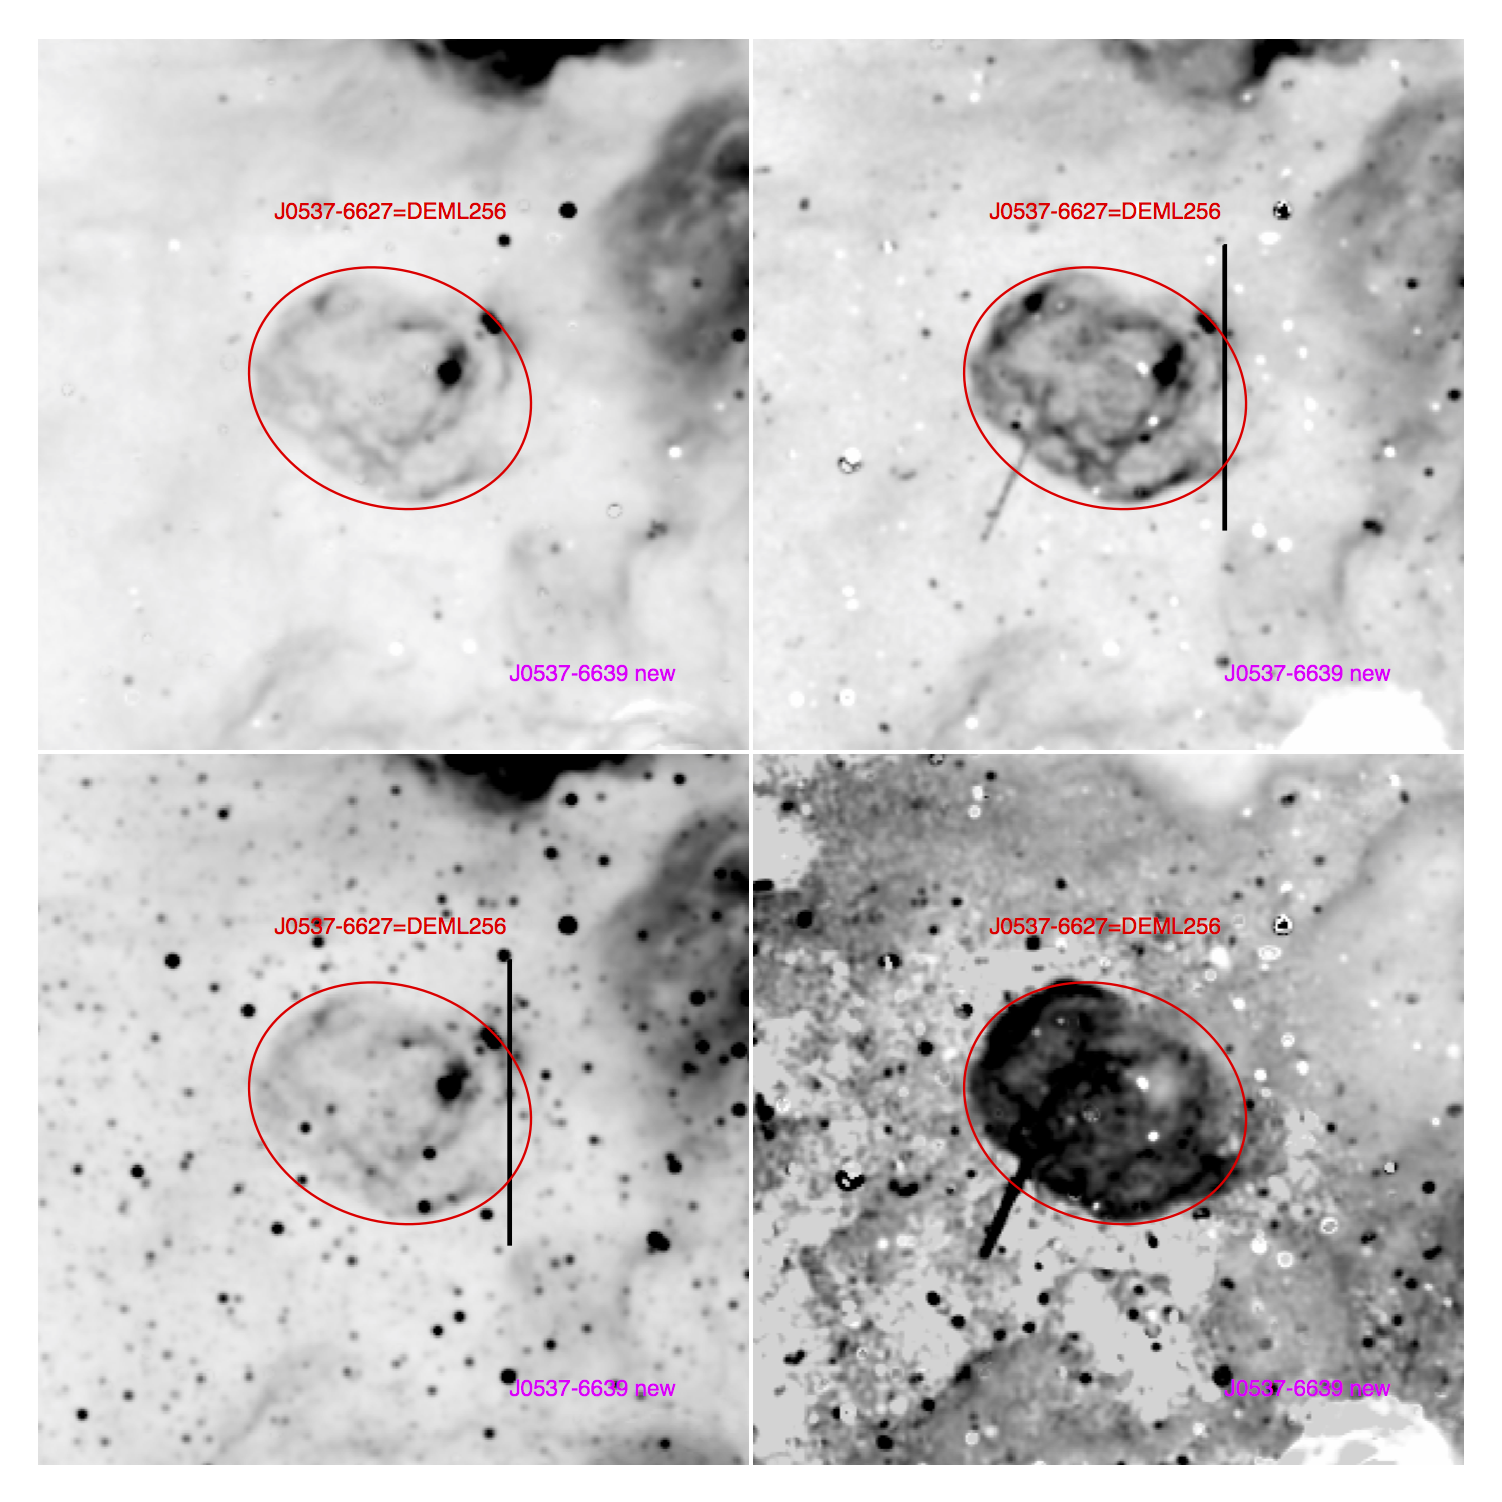
\includegraphics[width=10.05cm]{snapshots/J0537-6627.png}
\end{figure}

\newpage
{\bf J0538-7004 (new)}  
 
Slit Center:  5:38:39.887  -70:04:13.737 N-S

Scan:  East

Scan rate:  

Date/Frames:

Exposure Times:  

\begin{figure}
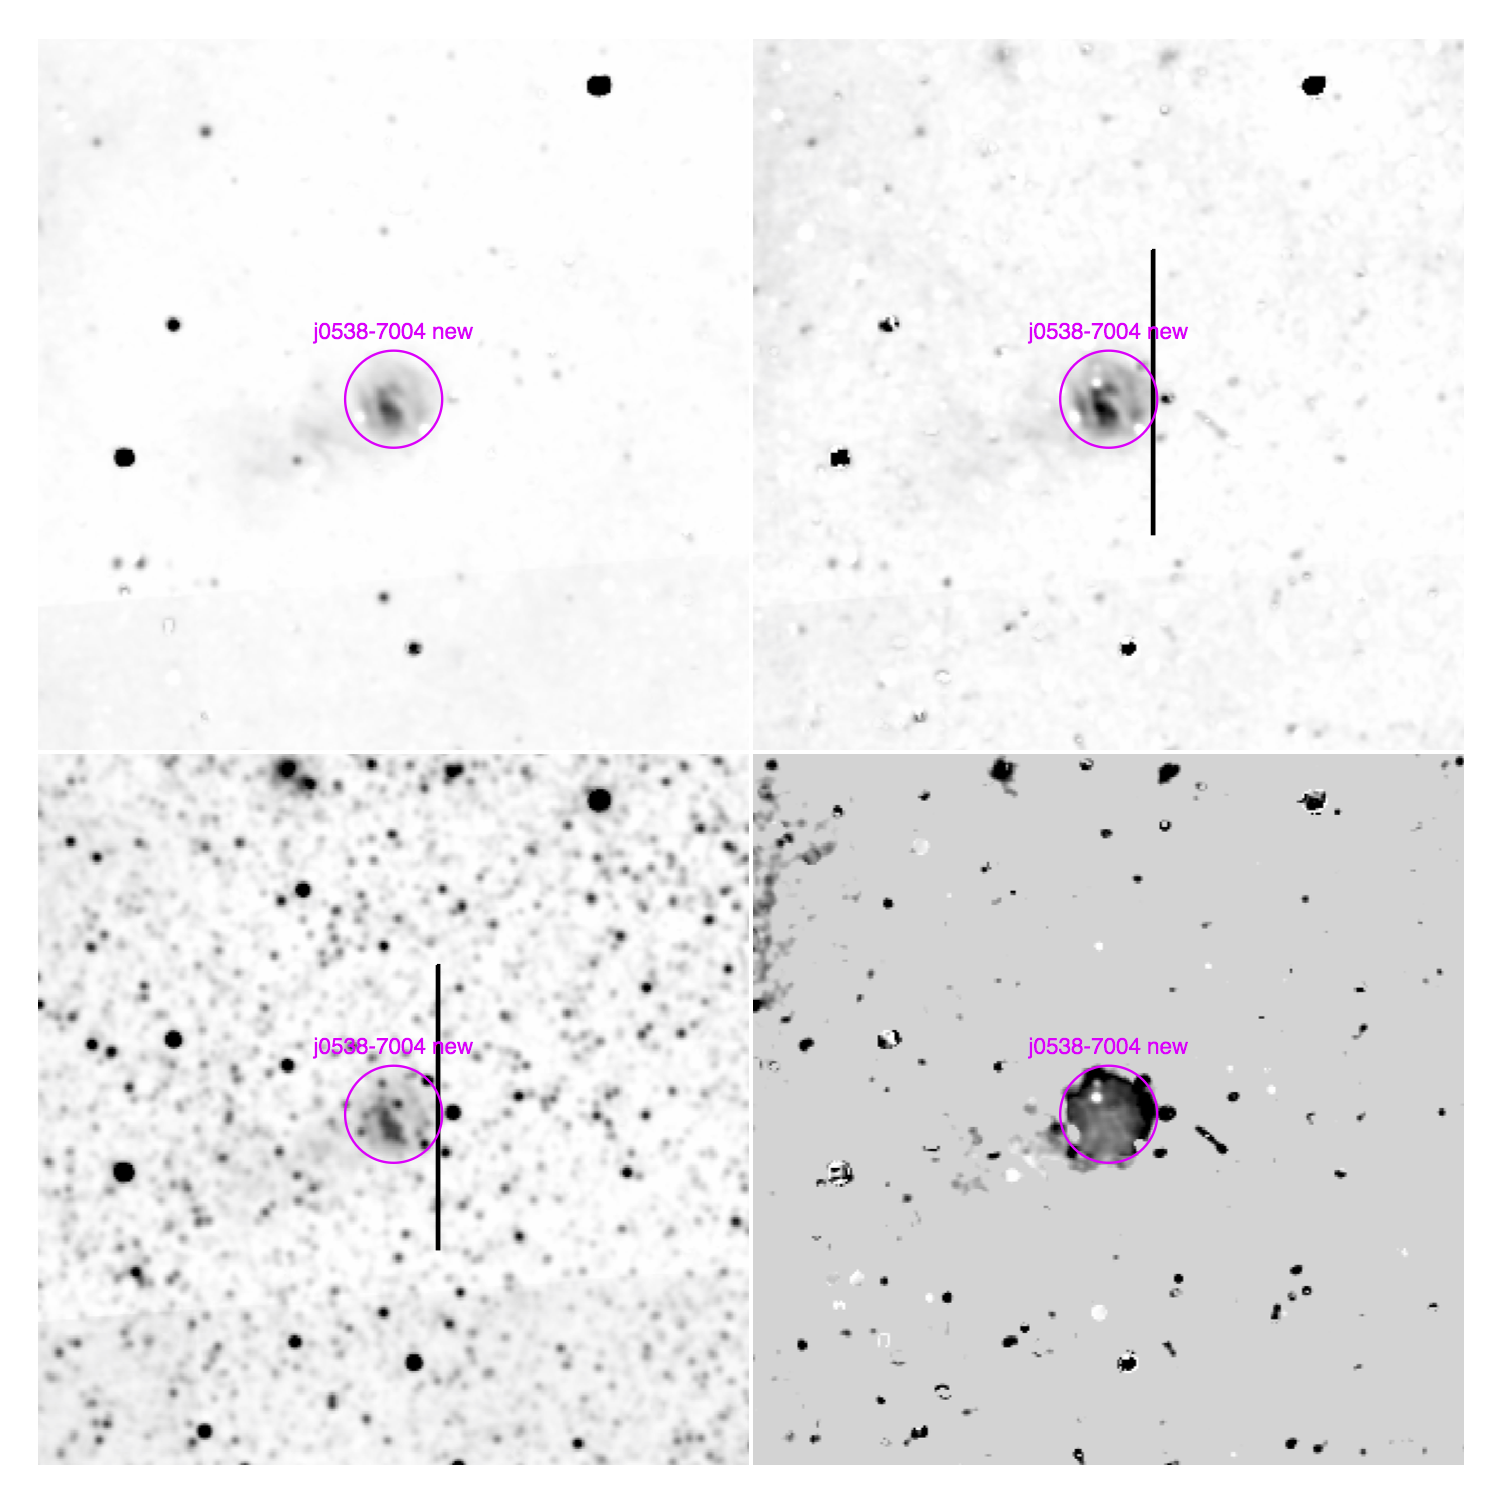
\includegraphics[width=10.05cm]{snapshots/J0538-7004.png}
\end{figure}

\newpage
{\bf J0540-6919 = B0540-69.3  (O-rich plerion; 5 arcmin field)}  
 
Slit Center:  5:40:09.612  -69:19:28.770 N-S

Scan:  East

Scan rate:  

Date/Frames:

Exposure Times:  

\begin{figure}
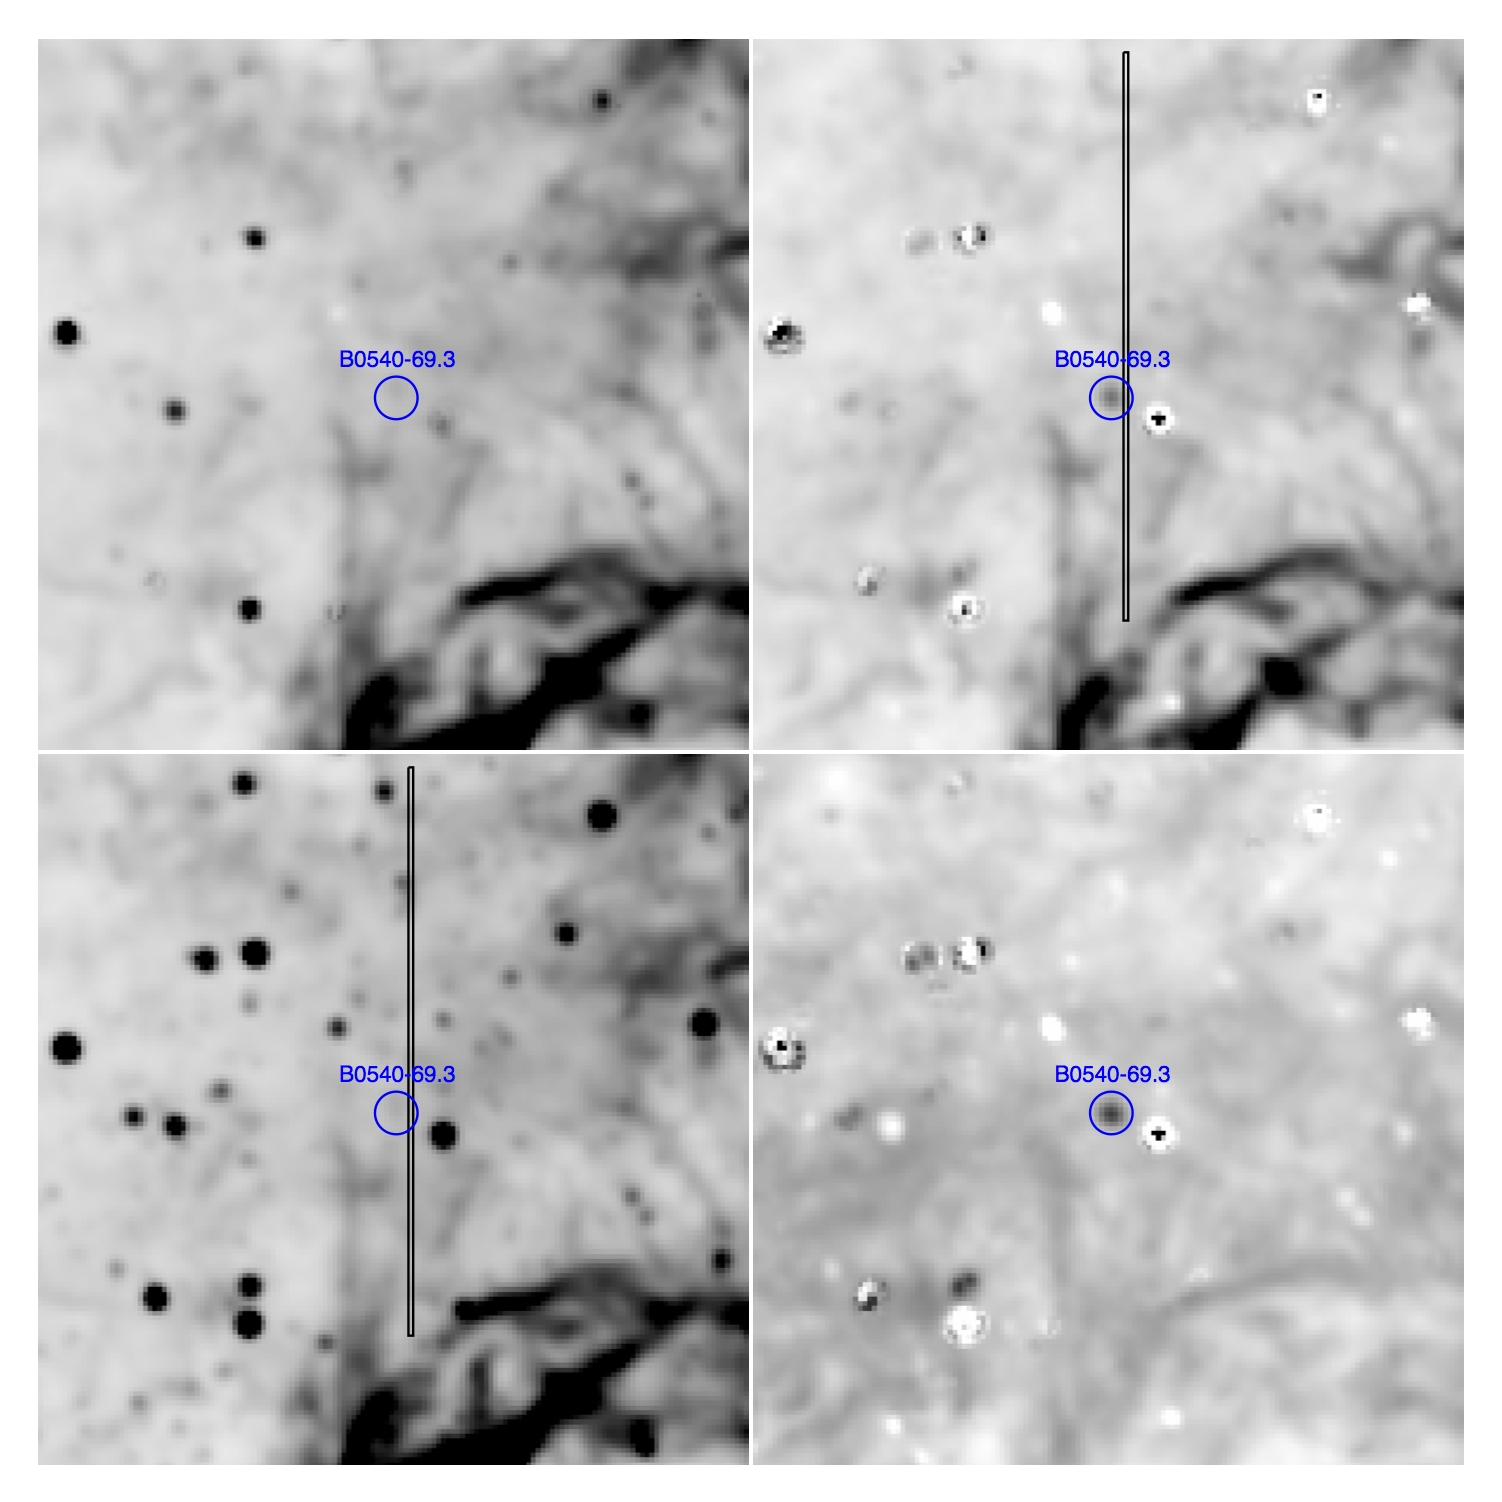
\includegraphics[width=10.05cm]{snapshots/B0540-693_5arcmin.png}
\end{figure}

\newpage
{\bf J0543-6858 = B0543-68.9 = DEML299}  
 
Slit Center:  5:43:10.442,-68:57:46.11 E-W

Scan:  South

Scan rate:  

Date/Frames:

Exposure Times:  

\begin{figure}
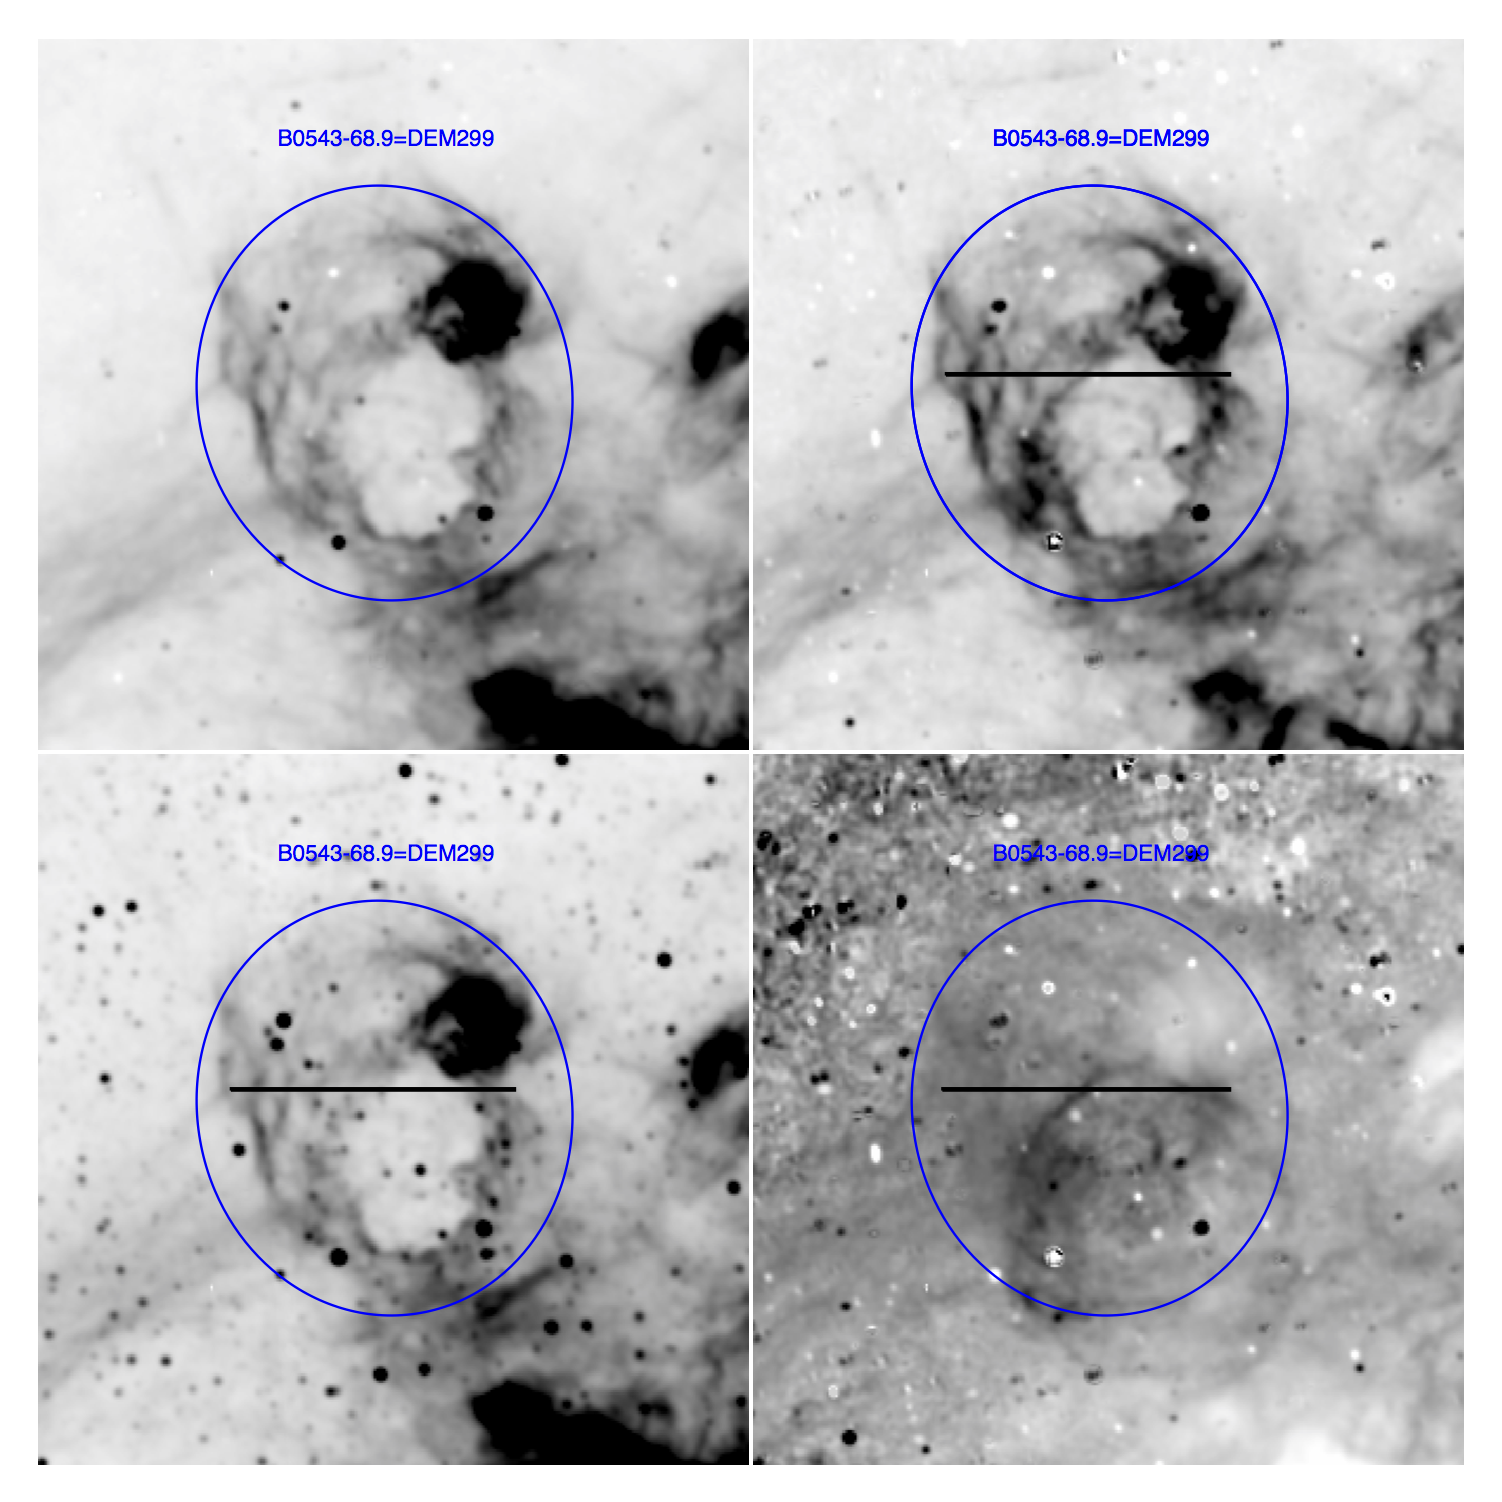
\includegraphics[width=10.05cm]{snapshots/B0543-689.png}
\end{figure}

\newpage 
 
{\bf J0546-6942 = B0547-69.7 = N135}

Slit Center:  5:47:10.057,-69:42:34.959  N-S

Scan:  West

Scan rate:  

Date/Frames:

Exposure Times:  

\begin{figure}
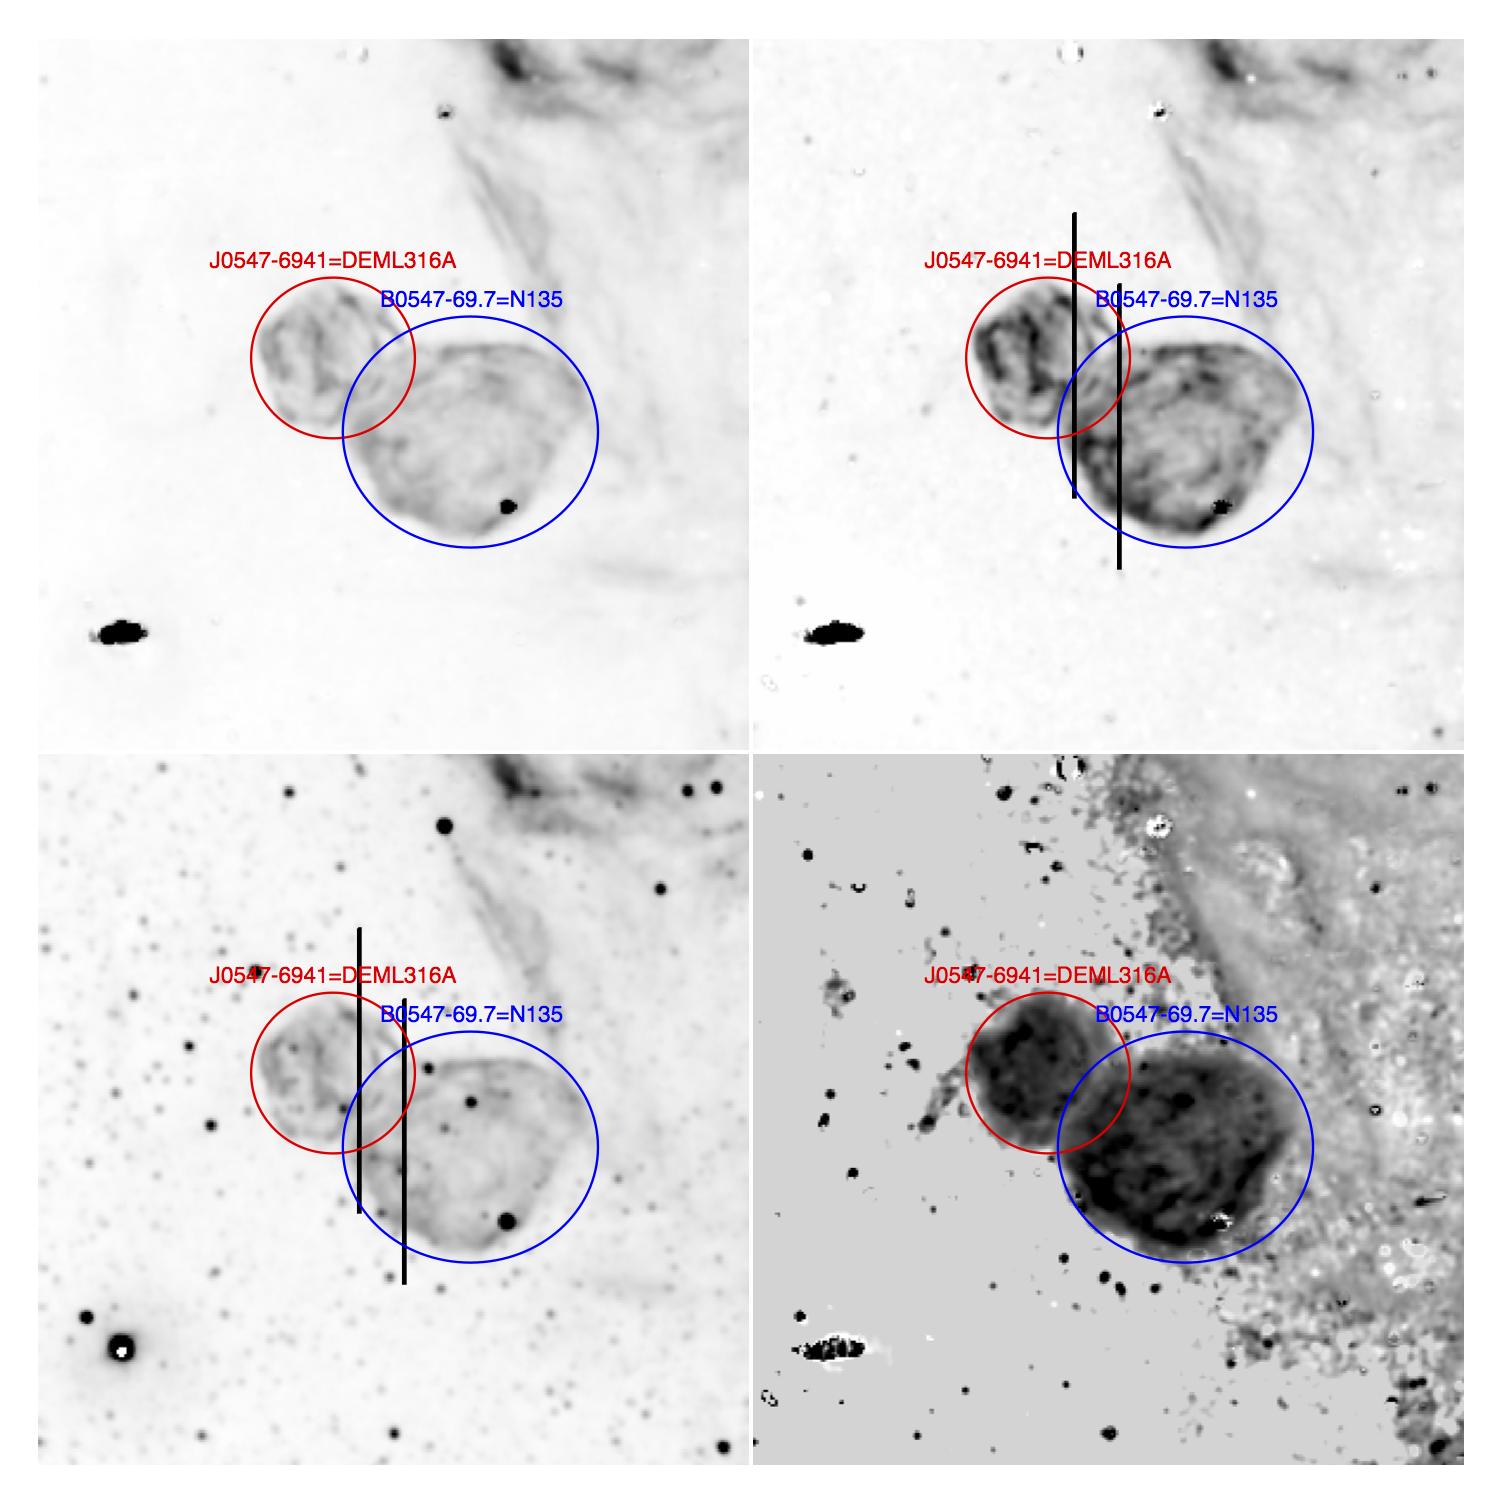
\includegraphics[width=10.05cm]{snapshots/B0547-697_double.png}
\end{figure}

\newpage 
 
{\bf J0547-6941=DEML316A}

Slit Center:  5:47:15.929   -69:41:30.947  N-S

Scan:  East

Scan rate:  

Date/Frames:

Exposure Times:  

\begin{figure}
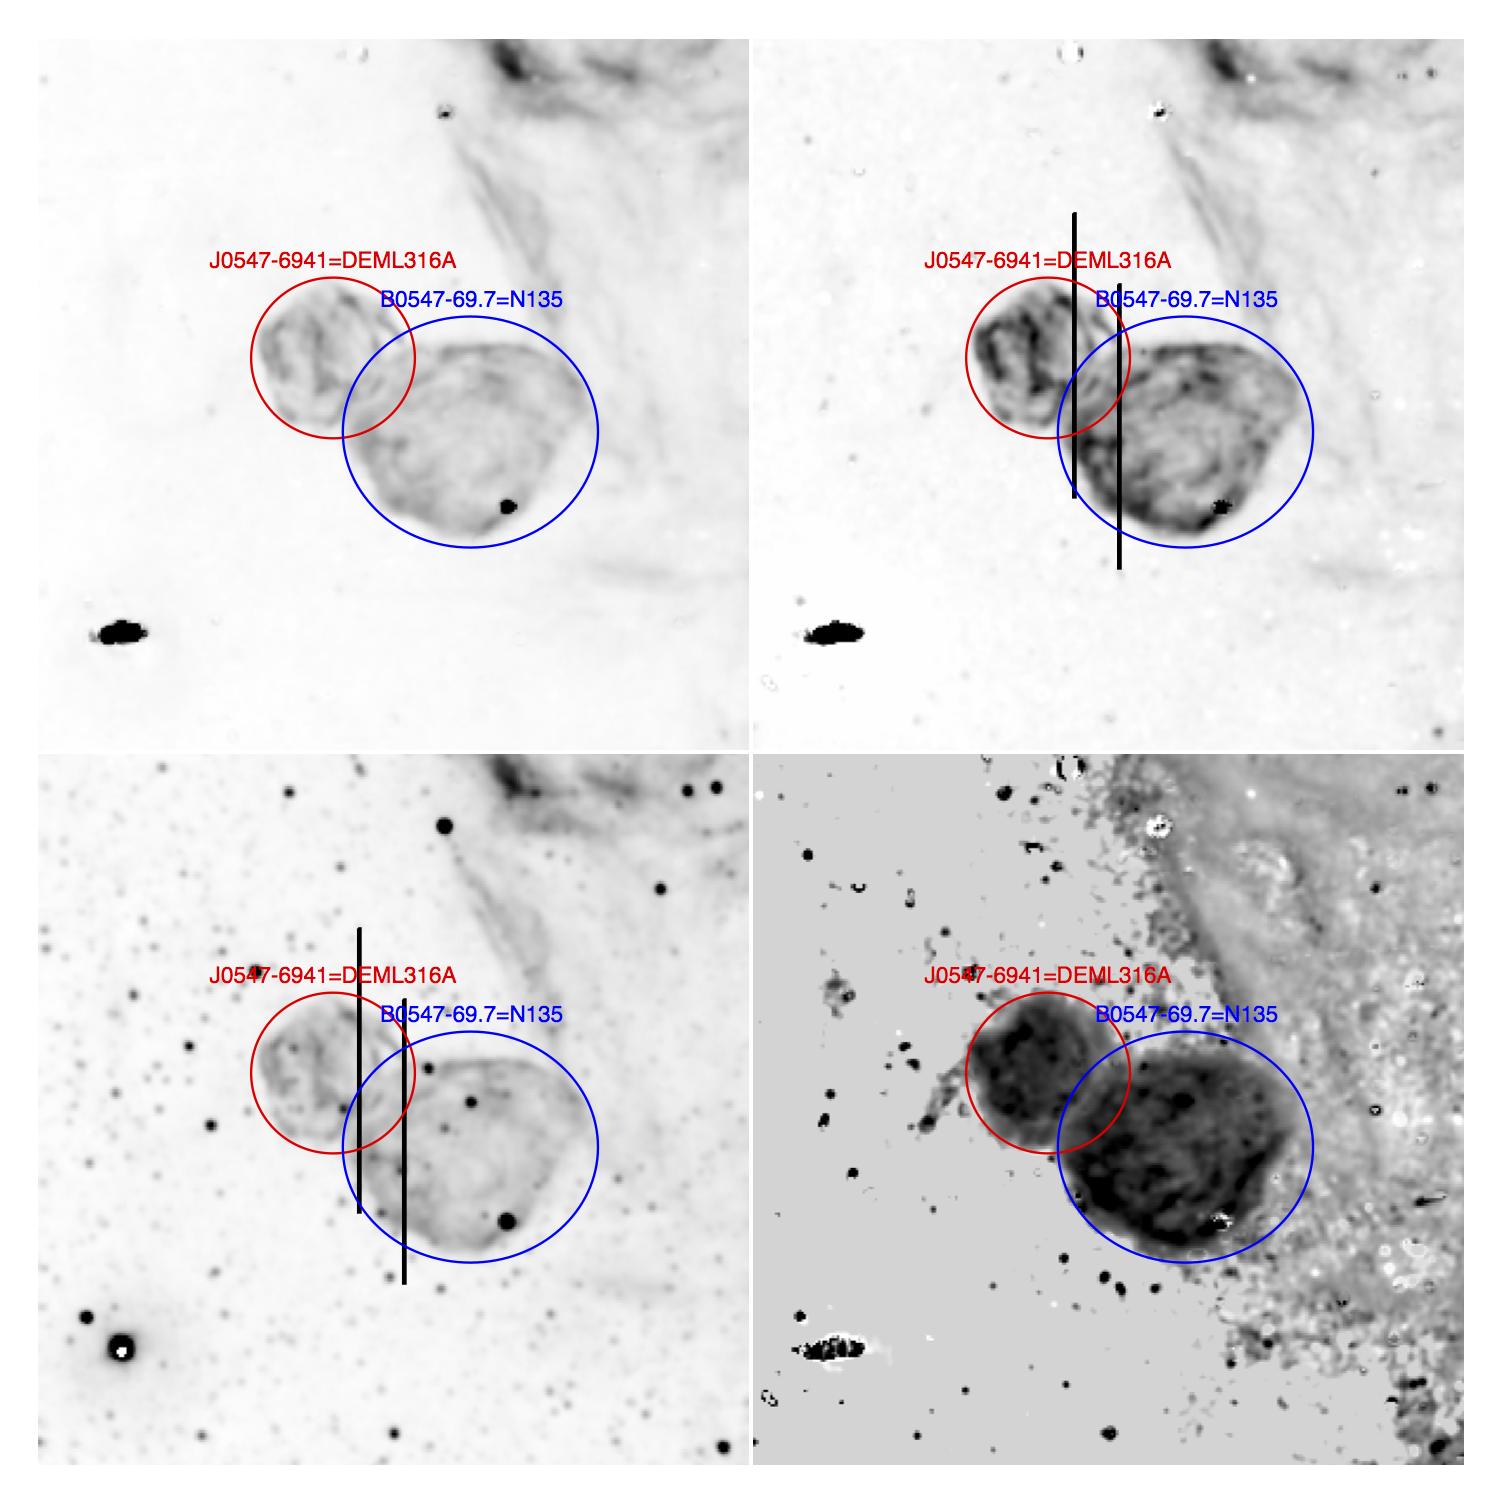
\includegraphics[width=10.05cm]{snapshots/B0547-697_double.png}
\end{figure}

\newpage 
 
{\bf J0547-7024 = B0548-70.4 (Balmer-dominated)}

Slit Center:  5:47:38.153   -70:25:05.964  N-S

Scan:  East

Scan rate:  

Date/Frames:

Exposure Times:  

\begin{figure}
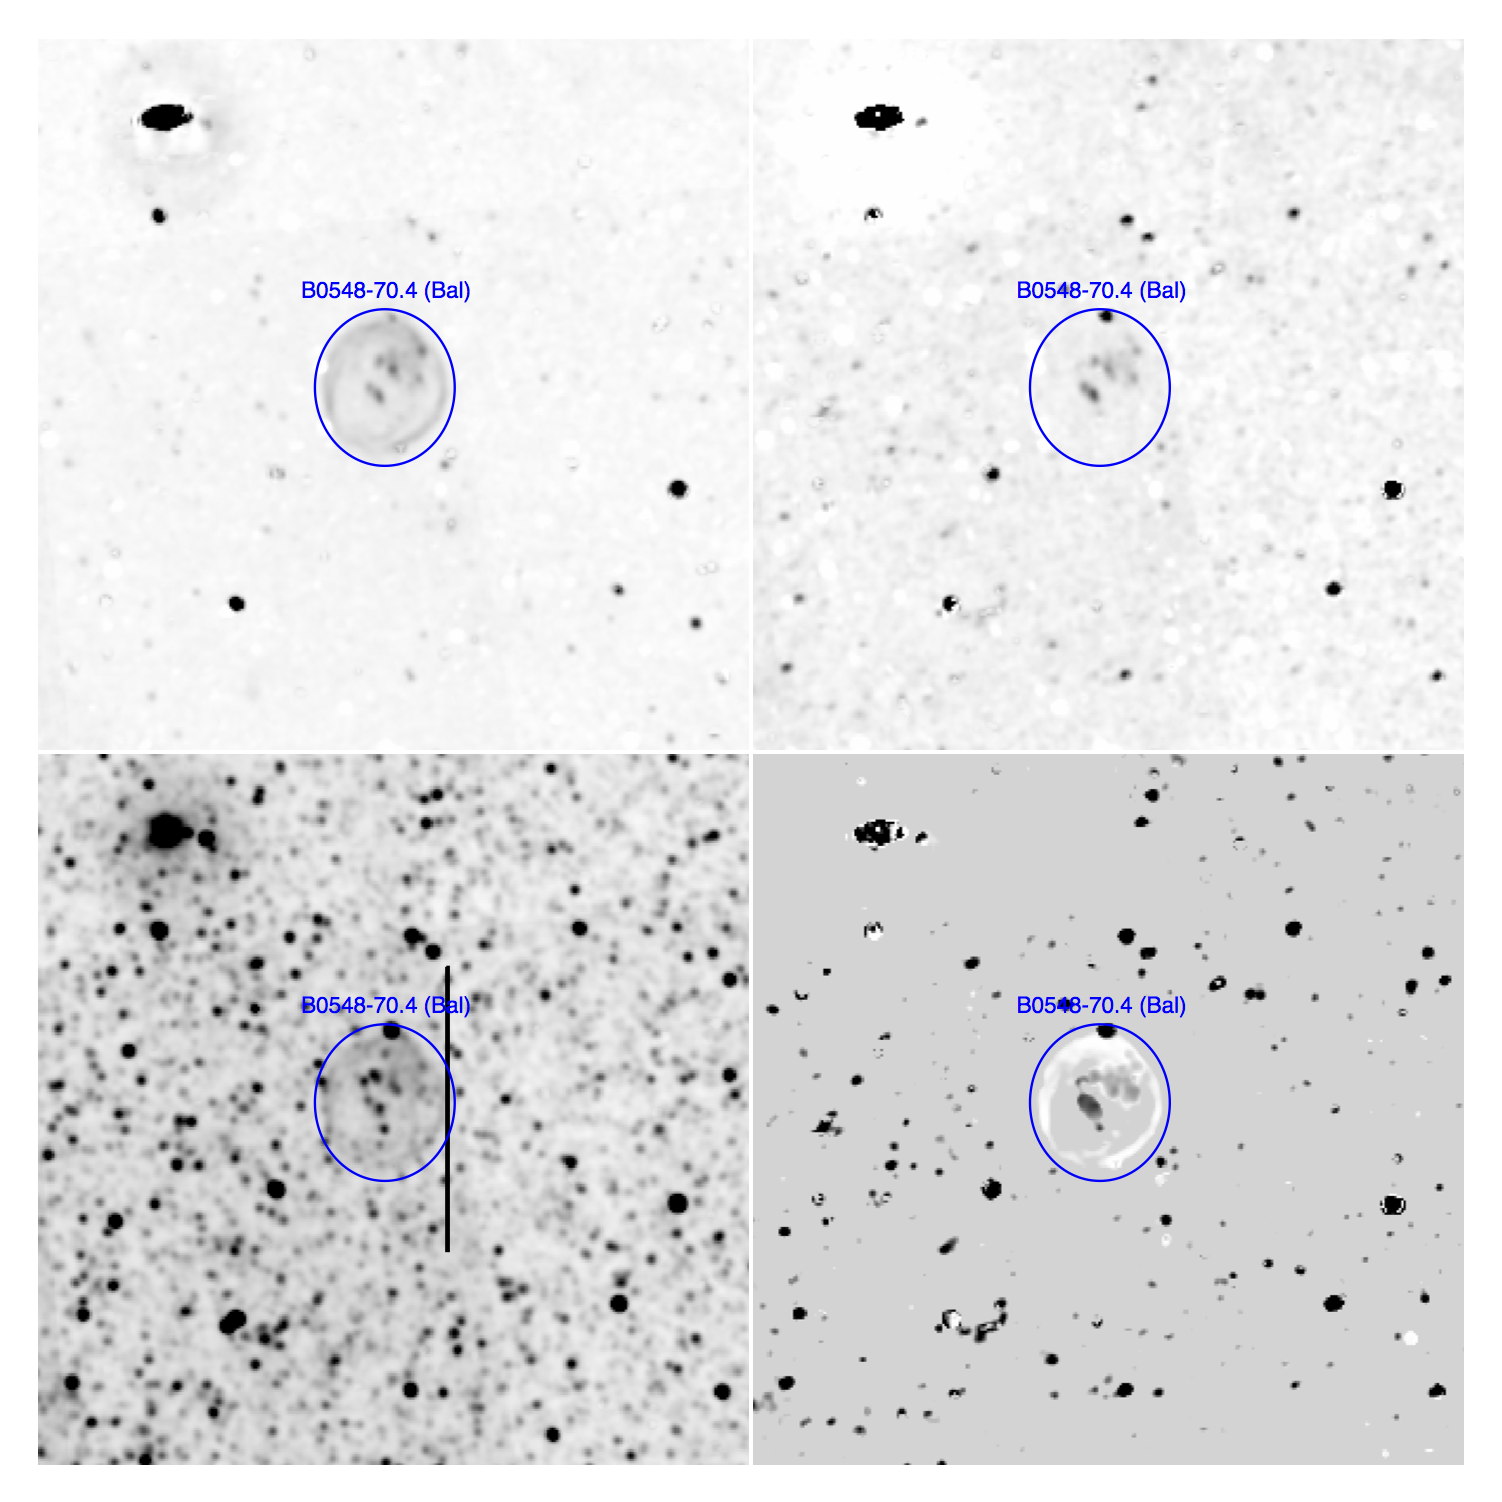
\includegraphics[width=10.05cm]{snapshots/B0548-704.png}
\end{figure}


\end{document}  